
\chapter{Generation of Meshes for the Multi-Scale Models}\label{sec:generation_of_meshes_for_multiscale}
Multi-scale models of skeletal muscles describe phenomena on different length scales and combine them into a single description. The phenomena are modeled by different sets of equations which need individual discretizations and solvers. For that, various geometrical meshes describing different physical domains are required.

The discretization considered in this work involves three-dimensional (3D) and one-dimensional (1D) meshes.
As a whole, muscles and tendons are treated as 3D domains. Muscle fascicles and myofibrils are represented by 1D fibers that are embedded in the 3D domain of the muscle.

The generation of the respective 1D and 3D meshes should be based on biomedical imaging data in order to represent actual human anatomy. The generated meshes should be of good quality such that finding numerical solutions with low error is possible. Good mesh quality usually involves mesh cells with similar lengths and angles. It should also be possible to easily partition the mesh into multiple, equally sized subdomains. This is required for efficient parallel computation.
The two requirements of good mesh quality and easy partitioning lead to the decision to employ \emph{hexahedral} elements and a \emph{structured} mesh for the 3D domains.

In this chapter, we present a workflow to construct meshes with the mentioned properties starting from biomedical data. We present novel algorithms to generate the required structured hexahedral meshes. This work contributes an implementation of the algorithms that can be used to construct all meshes needed for our biomechanical simulations.

\section{Overview and Notation of Required Meshes}\label{sec:overview_and_notation_of_required_meshes}
In the following, we summarize the meshes generated and used in this thesis and introduce their notation used in the following discussions.

The domain of the muscle belly is denoted by $\Omega_M$. A layer of fat and skin tissue is located on top of the muscle belly. It is denoted as the body domain $\Omega_B$.
The muscle belly is attached to tendons on both longitudinal ends. The tendon domains are denoted by $\Omega_{T,1}$ and $\Omega_{T,2}$. These domains are all subspaces of the 3D Euclidean space: $\Omega_M,\Omega_B,\Omega_{T,i} \subset \R^3$.

Additionally, a number $n_f$ of individual muscle fibers $\Omega_{F,i} \subset \R^3$ for $i \in \{0,\dots,n_f\}$ is introduced. Each fiber is a 1D manifold embedded in the 3D domain, i.e., $\Omega_{F,i} \subset \Omega_M$. \Cref{fig:fibers_domains} summarizes the notation of the domains.

\begin{figure}%
    \centering%
    \def\svgwidth{8cm}%
    \input{images/fiber_creation/domains.pdf_tex}%
    \caption{Visualization of the computational domains in a simulated muscle: tendons $\Omega_{T,1}, \Omega_{T,2}$, muscle belly $\Omega_M$, body domain $\Omega_B$ and fiber domains $\Omega_{F,i}$.}%
    \label{fig:fibers_domains}%
\end{figure}%

For the application of the finite element method (FEM), we create meshes for each of these domains. Formally, a 3D mesh $\Omega_\text{3D}$ is given by a number of 3D elements $\{U_{\text{3D},i}\}_{i=1,\dots,n}$ with $U_{\text{3D},i} \subset \R^3$ such that their disjoint union approximates the domain,
$\dot{\bigcup}_{i=1}^{n} U_{\text{3D},i} \approx \Omega_\text{3D}$. Similar holds for 1D meshes.

The elements are non-overlapping and can be defined by nodes and edges. In the discretizations used here, no hanging nodes are allowed, i.e., at any node all adjacent elements share the node.

Furthermore, only structured, hexahedral meshes are considered in this chapter.
A 3D structured mesh is isomorphic to a 3D cartesian grid with equidistant elements. 
This has advantages for programmatically indexing nodes and elements as well as for parallel partitioning of the domain.
\Cref{fig:fiber_creation_decomposition} shows an example of a 3D structured mesh that is partitioned into twelve subdomains. The subdomains are constructed by planar cuts through the structure of the mesh. These cuts are typically defined in a way that the resulting subdomains have similar numbers of 3D elements and, thus, every process gets a similar portion of the total computational load.

The number $n$ of 3D elements is the product of the numbers $n_i, n_j$ and $n_k$ of elements in the three coordinate directions $x,y$ and $z$ of the cartesian grid,
 i.e., $n = n_i\,n_j\, n_k$.
Each element can be indexed by a triple $(i,j,k)$ of indices with the ranges $i \in \{0,\dots,n_i-1\}, j \in \{0,\dots, n_j-1\}$ and $k \in \{0,\dots,n_k-1\}$. 
In the simulation program, typically, consecutive indices $\iota$ are used that iterate over all elements $\iota \in \{0,\dots,n-1\}$ and are obtained from the index triples by the mapping 
$(i,j,k) \mapsto \iota = k\,n_i\,n_j + j\,n_i + i$.

\begin{figure}%
  \centering%
  \begin{subfigure}[t]{0.5\textwidth}%
    \centering%
    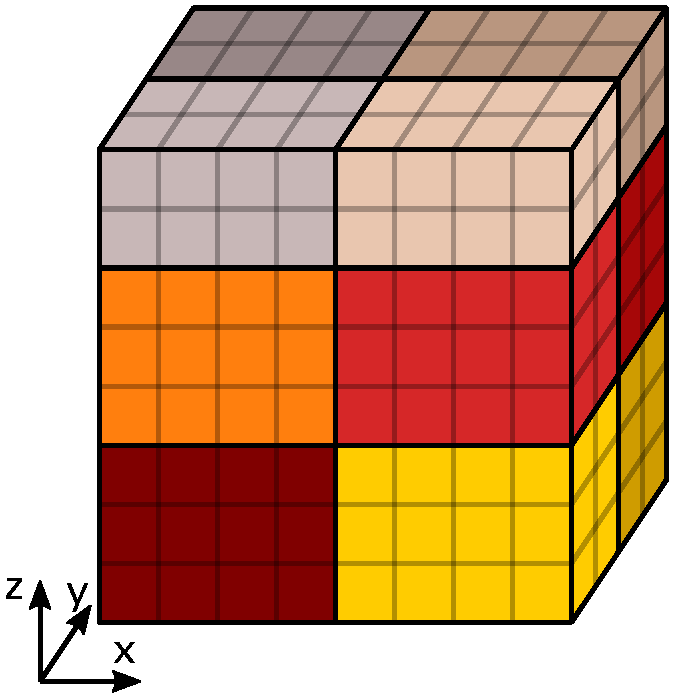
\includegraphics[width=\textwidth]{images/fiber_creation/decomposition.pdf}%
    \caption{Parallel decomposition of a 3D mesh with $n_x \times n_y \times n_z = 8 \times 4 \times 8$ elements into $2 \times 2 \times 3=12$ subdomains.}%
    \label{fig:fiber_creation_decomposition}%
  \end{subfigure}
  \quad
  \begin{subfigure}[t]{0.45\textwidth}%
    \centering%
    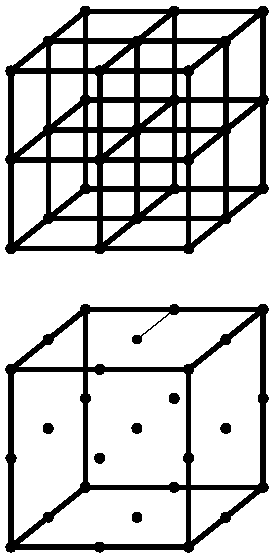
\includegraphics[width=0.6\textwidth]{images/fiber_creation/quadratic_elements.pdf}%
    \caption{Top: a linear 3D mesh with eight elements, bottom: a single quadratic element, which uses the same nodes as the linear 3D mesh at the top.}%
    \label{fig:fiber_creation_quadratic_elements}%
  \end{subfigure}    
  \caption{Structured 3D meshes that are used in the simulations: parallel partitioning and construction of quadratic elements.}%
  \label{fig:quadratic_elements_decomposition}%
\end{figure}%

The elements of such a mesh can have different numbers of \emph{degrees of freedom (dof)} depending on the desired spatial order of consistency of the finite element discretization. The number $n_{\text{dofs,}d\text{D}}$ of dofs in a $d$-dimensional element is computed from the number $n_{\text{dofs,1D}}$ of dofs along one coordinate direction of the element as $n_{\text{dofs,}d\text{D}} = n_{\text{dofs,1D}}^d$.
Consequently, linear elements have two dofs in 1D meshes and eight dofs in 3D meshes. Quadratic elements have three dofs in 1D and 27 dofs in 3D.

The dofs are located at the \emph{nodes} of the elements. In linear and quadratic elements, every node corresponds to a single dof. While the nodes form the \say{corners} of linear 3D elements, they are also located on the faces and in the interior of quadratic 3D elements. \Cref{fig:fiber_creation_quadratic_elements} shows a mesh with $2 \times 2 \times 2$ linear 3D elements at the top. The same 27 nodes can be used to define a single quadratic 3D element as shown at the bottom of \cref{fig:fiber_creation_quadratic_elements}. 

It is sufficient to develop a method for constructing structured 3D meshes with linear elements. 
Higher order elements can be geometrically constructed by using the nodes of multiple adjacent linear elements.
To generate both linear and quadratic elements, we always begin with generating a mesh with even numbers $n_i,n_j$ and $n_k$ of elements in the coordinate directions. Then, linear and quadratic meshes can be extracted from the set of nodes. Similarly, a linear 1D mesh with an even $n_i$ can be easily converted into a quadratic 1D mesh.

The next sections describe workflows and algorithms to construct 3D meshes for the domains $\Omega_M,\Omega_B,\Omega_{T,i}$ and 1D meshes for the fibers $\Omega_{F,i}$ based on anatomical information. \Cref{sec:fiber_meshes_related_works} gives an overview over available meshing software tools and existing algorithms in literature. Then, \cref{sec:preprocessing_of_the_muscle_geometry} presents a workflow to extract a smooth surface representation from anatomical imaging data. In \cref{sec:ser_alg_meshes}, two serial algorithms are presented to generate 3D meshes and 1D fibers meshes. The next section, \cref{sec:parallel_algorithm}, extends these serial algorithms formulating a parallel algorithm and shows and discusses results. Finally, \cref{sec:meshes_summary_and_conclusion} gives a summary and concludes this chapter.

\section{Related Work}\label{sec:fiber_meshes_related_works}

Generating volumetric meshes for domains enclosed by a given surface is a task that is frequently needed in computational science. It is a preprocessing step whenever spatially discretized models have to be solved numerically. In consequence, a vast amount of literature has addressed this algorithmic task and various approaches and methods have been proposed. Moreover, numerous software packages that solve this problem exist. Especially tools for Computer Aided Design and Engineering (CAD/CAE) as well as free and commercial preprocessing tools and finite element solver software include functionality to generate meshes from given surfaces.

An example from the biomechanical domain is \cite{untaroiu2013finite}. The study develops a finite element model of the lower limb of an occupant of a car with the aim to investigate injury scenarios during traffic crashes.
The lower extremity geometry was obtained by computer tomography (CT) and magnetic resonance imaging (MRI) scan data of a 50th percentile male volunteer. Different meshes of bones and ligaments were created using the three tools IA-FEMesh \cite{grosland2009ia}, TrueGrid \cite{TrueGrid} and Hyper-Mesh \cite{Hypermesh} which will be outlined in the following.

\emph{IA-FEMesh} (University of Iowa, Iowa City, USA) is an open source tool to generate hexahedral meshes \cite{grosland2009ia}. It provides an interactive environment where existing geometries can be loaded. In a visualization window, bounding boxes, called blocks, can be positioned such that they contain the whole geometry. A structured grid on the block is then projected onto the surface of the geometry. Multiple blocks can be placed to account for more complex geometries. The resulting surface mesh is improved using Laplacian smoothing which equalizes the edge lengths of the elements.
The interior nodes are generated using interpolation.
The result is a structured mesh if only one block is used or an unstructured mesh if multiple blocks are used. Further operations to manage mesh density, visually manipulate the meshes and add material properties, load and boundary conditions are available. The model can be exported in a file format for finite element analysis with ABAQUS (Dassault Systèmes, Vélizy-Villacoublay, France) \cite{ABAQUS}.

The second tool is \emph{TrueGrid} (XYZScientific Applications, Livermore, USA) \cite{TrueGrid}. It is a commercial toolkit to generate hexahedral meshes. The project was started in the early 1990s as the successor to the even older preprocessor software \emph{INGRID}. Similar to \emph{IA-FEMesh}, a projection method and a multi-block technique are used. Some effort has been put into dealing with holes and sewing together dissimilar blocks.

The third tool is \emph{Hyper-Mesh}, the commercial pre- and postprocessing toolkit of Hyperworks (Altair HyperWorks, Troy, USA) \cite{Hypermesh}.
Altair sells infrastructure and solvers for a multitude of physics and is targeted at a wide range of industries. 
Being a commercial vendor, information about the internals of their preprocessing software are hardly provided.

More meshing software exists, such as CGALmesh \cite{Jamin2015CGALmesh} for tetrahedral meshes. The package gives quality guarantees of their generated meshes and includes four mesh optimization algorithms to further improve the mesh quality.

Another application-oriented work dedicated to the use of commercial tools is \cite{Ellankavi2018}. A workflow for patient-specific modeling, simulation and analysis of the interaction between a residual lower limb stump and the socket of a prosthesis is presented. Imaging data were taken from magnetic resonance diffusion tensor imaging where also the preferred diffusion direction of water molecules along muscle fibers is captured. The open source tool MedInria (National Institute for Research in Digital Science and Technology (Inria), France) \cite{vichot2012cardiac} was used to extract muscle fibers. The residual limb data were processed using the commercial 3D image segmentation software Simpleware ScanIP (Synopsys, Mountain View, USA). Auxiliary tasks were performed using MATLAB (MathWorks,	Natick, USA) scripts. The commercial multiphysics solver LS-DYNA (LSTC/Ansys, Canonsburg, USA) was used for the simulations.

Commercial tools usually have the advantage that more development effort was put into them, than is possible for open source codes from the scientific community. This often leads to more robust and user-friendly software. An advantage of open source software is that the used algorithms are disclosed to everyone. They are often well documented or described in a publication. This allows to assess the expected quality of the generated meshes. Conversely, commercial vendors usually have no interest in revealing their internal algorithms.

For our simulation, structured, hexahedral meshes are needed. Several of the described tools are able to generate hexahedral meshes, however the meshes are typically unstructured. For our special need of 1D muscle fibers embedded in a 3D mesh, we develop our own method that is based on the ideas of existing algorithms. In the following, an overview over the algorithmic common knowledge of creating simplex meshes and hexahedral meshes is given as a basis.

% other 3D meshing
% tets
Triangulating a 2D domain is the archetype of mesh creation. The triangulation named after B. Delaunay was formulated in 1934 \cite{delaunay1934sphere}. For a given set of points, it maximizes the minimum angle of the triangles and, thus, avoids small angles. Therefore, a guarantee on the quality of the triangulation is given.

In 1995, J. Ruppert presented the Delaunay refinement algorithm \cite{Ruppert1995}, which constructs a Delaunay triangulation conforming to prescribed connected points. This algorithm is still commonly used and also part of numerous derived meshing techniques.

In 1997, P. Chew developed an algorithm for meshing a 3D domain with tetrahedra \cite{chew1997guaranteed} and proved that the aspect ratio of the tetrahedra is bounded, i.e., degenerate, \say{flat} tetrahedra, called slivers, are avoided.

The authors of \cite{Alliez2005Variational} propose a variational approach to triangulation where a quadratic energy function is minimized. During minimization both vertex positions and connectivity are optimized. This leads to better quality meshes than by simple Delaunay triangulations.

% tets to quads:
Hexahedral meshes can be obtained from certain tetrahedral meshes by splitting up each tetrahedron into four hexahedra. This is discussed in \cite{eppstein1999linear}. A remaining issue is that the generated meshes from this procedure are highly unstructured and some hexahedra have poor quality, whereas the goal would be to construct elements that are almost equilateral.

% hexs
A different approach is to directly generate a hexahedral mesh for the given surface geometry.
The survey in \cite{owen1998survey} identifies four different strategies for generating unstructured hexahedral meshes.

The first one is a \emph{grid-based} approach. It was introduced in \cite{schneiders1996grid,schneiders1997algorithm}. The interior of a given solid is filled with a regular and cartesian grid of as many hexahedral elements as fit into the space. Then, the gaps at the surface are filled with additional elements. This method is robust but can lead to poor quality elements near the surface. 
%The orientation of the interior grid highly depends on the orientation of the initial surfaces and may not be the natural orientation of the given volume.

The second approach for generation of hexahedral meshes are \emph{medial surface methods} \cite{price1995hexahedral, price1997hexahedral}. First, the volume is decomposed into subregions by medial surfaces such that the resulting domains are one of only 13 possible types. Predefined templates are used to fill the domains with hexahedral elements. Then, the continuity between the domains is ensured using linear programming. This approach gives good results for some geometries but has robustness issues when general geometries are considered.

The third approach is called \emph{plastering}. It was first described by \cite{blacker1993seams} and continued by \cite{staten2006unconstrained,staten2010unconstrained}.
It is a moving-front method where hexahedral elements are placed in layers starting at the boundary and moving towards the interior. Intersection of faces has to be detected when the fronts meet in the interior and rules for connecting to existing faces have to be defined.
During this process, complex shaped voids can occur in the interior. When it is no longer possible to fill the voids with hexahedra already placed elements have to be removed.
A new method, called unconstrained plastering, starts from an unmeshed volume boundary. The approach has general robustness issues and is not guaranteed to find a solution for arbitrary boundaries.

The forth approach is \emph{whisker weaving}, introduced by \cite{tautges1996whisker} and extended by \cite{ledoux2008extension,kawamura2008strategy}. Here, the dual of the hexahedral mesh is considered. The dual consists of the three surfaces per hexahedron that lie in the planes of symmetry. The surfaces of all hexahedra form topological loops. 
The principle is now to first construct the dual of the mesh, which can be determined from the given boundary surface. Then, the actual hexahedral mesh is created from the dual, using the surfaces as guides where to place the elements.
The dual forms topological loops inside the volume. One important criterion for generating good quality meshes is that self-intersections of these loops are resolved in a first step.
The approach, used with subsequent smoothing, can produce meshes of good quality. However, no guarantee is given. One problem is that the resulting mesh depends on the quality of the surface mesh and that the number of nodes can increase significantly during the method.

For the whisker weaving method and for some plastering methods, a quadrilateral mesh of the surface is required. Algorithms for creating high quality quadrangulations of closed surfaces exist \cite{dong2005quadrangulating,Kovacs2011Anisotropic,Bessmeltsev2012,Meng2016Consistent}.

Other approaches start with 3D volumetric medical imaging data instead of surfaces. In \cite{Zhang2003,Zhang20053DFiniteElementMeshing}, adaptive tetrahedral and hexahedral meshes are created from volumetric data using octree subdivision. The method avoids hanging nodes and allows a feature sensitive adaptivity. While adaptive meshing methods can reduce the number of elements in the interior of the volume, a problem is that the worst quality elements are generated at the boundary, the location where the solution in a finite element study usually is most interesting.

\nocite{Gregson2011}

Multiple reasons make the previously outlined approaches unsuited regarding the needs for our parallel muscle simulation. 

(i) The generated meshes are unstructured. When performing domain decomposition for parallel computing on unstructured meshes, graph-partitioning methods have to be used. Storing an unstructured mesh requires storage of element adjacency information. Partitioned meshes additionally require storage of the adjacent processes. In contrast, structured meshes can be trivially decomposed and stored efficiently. A decomposition can be represented in memory by a very low number of parameters.

(ii) The presented methods are designed for hexahedral meshing of arbitrary volumes. Robustness and mesh quality at the same time remain issues that are not completely solved for most of the algorithms. Often, expensive smoothing steps are needed to increase mesh quality.

(iii) In general, either no assumption can be made about orientation or alignment of hexahedra in the interior, or, for the grid-based approach, the elements at the surface have poor quality. Having a mesh that is consistently aligned with, e.g., the main diffusion direction or the preferential direction of the anisotropic material or the muscle fibers can reduce numerical errors in the finite element solution.

Consequently, a more scenario specific solution is needed that can avoid the mentioned issues. Such solutions can also be found in the literature. An example is \cite{blemker2005three}, where 3D finite element models for various complex muscle geometries around the hip are generated from magnetic resonance images. Segmentation and surface mesh generation are performed using the old, unmaintained software \emph{Nuages} (Inria, France) \cite{Nuages}.
Then, a 3D hexahendral mesh is generated using TrueGrid. A structured template mesh on a unit square is mapped to the horizontal slices of the muscle geometry that resulted from the segmentation. After mesh smoothing, the slices are connected vertically to form a 3D mesh. 
Fiber directions are described by Bezier curves in a reference volume and mapped to the muscle geometry using the same mapping. The fiber direction then are used in a transversely-isotropic material formulation. Simulations are performed using the finite element solver \emph{Nike3D} (Lawrence Livermore National Lab, Livermore, USA) \cite{Nike3D}.

We base our work on this study and use a similar mapping from a template mesh to the actual muscle volume. In comparison to \cite{blemker2005three}, we use an improved mapping based on harmonic maps, which potentially leads to better quality meshes on the slices of the muscle. Instead of the unit circle template mesh, we experiment with different reference meshes and evaluate their quality.

In the study of \cite{blemker2005three}, fiber directions are defined based on anatomically assumed directions.
However, the definition is carried out on the cuboid reference geometry. This means that the authors mentally morph the muscle geometry into the reference geometry in order to define fiber directions, using their expertise. Then, the fiber directions together with the cuboid are transformed back to the actual geometry. This approach simplifies the definition of the fibers. However, defining the fiber direction directly on the muscle geometry can lead to better results. Thus, our approach is to automatically estimate fiber directions and define fibers directly in the muscle domain. At the same time, the 3D mesh and 1D fibers are aligned in our work to allow for better numerical and data structure properties of the discretization. 

The definition of fiber directions follows a method proposed in \cite{Choi2013}. 
The directions are assumed to follow a divergence free vector field. Such a field can be created by taking the gradient of the solution of the Laplace equation. Neumann boundary conditions are defined at the attachment points of the muscle tendon complex. The solution of the Laplace equation corresponds to the pressure values of a potential flow. Its gradient corresponds to the velocity and individual fascicles or fibers can be obtain by tracing streamlines through the velocity field.
This approach is extended and validated by the studies in \cite{Inouye2015} and \cite{Handsfield2017}. We incorporate this method into our workflow.

\section{Preprocessing of the Muscle Geometry}\label{sec:preprocessing_of_the_muscle_geometry}

The first step towards creating a structured mesh is to obtain a representation of the surface of the muscle. 
Starting point is a human biomedical imaging data set. In this section, two possible workflows are presented how to extract the muscle and tendon surfaces from imaging data. 
The two workflows are visualized in \cref{fig:scheme_preprocessing}. The workflow using the branch on the left side in \cref{fig:scheme_preprocessing} is automized but only works for the particular data set and extracting the biceps muscle.
The right branch involves manual steps and is applicable for any muscle geometry.

% overview over subsections

\begin{figure}%
  \centering%
  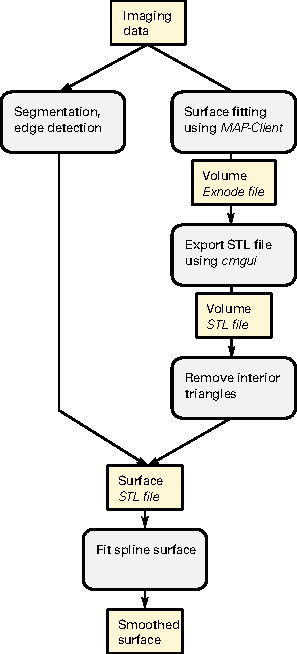
\includegraphics[height=15cm]{images/fiber_creation/scheme_preprocessing.pdf}%
  \caption{Workflow of generating a surface representation of the muscle and tendons from imaging data. Operations and intermediate results are shown as gray and yellow boxes, respectively. Two alternatives are given by the two branches. On the left, the imaging data are automatically processed to directly retrieve points on the surface of the muscle. The right branch achieves the same with three steps of which the first one involves manual adjustments. At the end, a spline surface smooths the collected data from both possibilities to yield the resulting surface representation.}%
  \label{fig:scheme_preprocessing}%
\end{figure}%

\subsection{Data Source}
Anatomic images provide the basis for the extraction of muscle geometries.
Our used data set originates from the Visible Human Project \cite{visible_human_male} of 
the United States National Library of Medicine. 
The project has published anatomic images derived from a male corps, among other data sets.
The data, known as \say{Visible Human Male}, were published in 1994.
Colored images of transversal cross sections were obtained by cryosectioning.
A total of \num{1871} images with dimensions of \num{2048} by \num{1216} pixels and 24 bit color depth visualize the whole human body. Parts of the upper arms are contained in approximately 500 of these images. The size of a pixel is \SI{0.33}{\milli\meter} in transversal direction and \SI{1}{\milli\meter} in axial direction. The size of the complete set of JPEG compressed images is \SI{772}{\mega\byte}. Cropping and selecting the relevant portions of the upper arm extracts a dataset with the size of \SI{35}{\mega\byte}.

An extract of an image of the upper arm is given in \cref{fig:vhp_image}. 
The location of biceps and triceps brachii muscles can be identified in the dark red tissue. For the biceps, the two muscle heads are visible, separated by the bright diagonal line from bottom left to top right. For the triceps, at least two of the three heads can be identified. The blue background is colored frozen gelatin that was needed during cryosection to stabilize the arms.

\begin{figure}%
  \centering%
  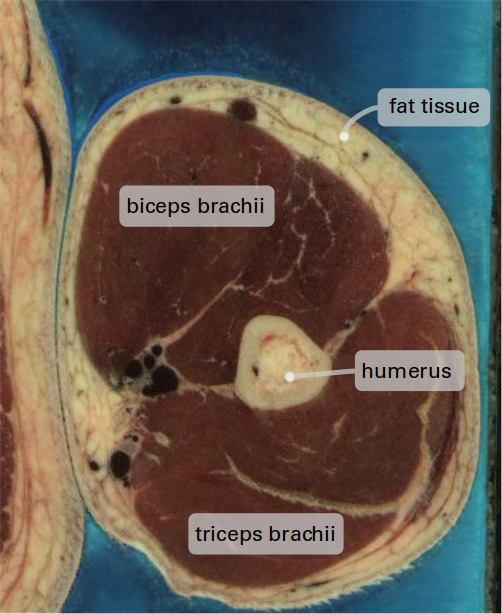
\includegraphics[height=10cm]{images/fiber_creation/vhp.png}% 0483
  \caption{Exemplary extract of image number 483 from the Visible Human Male. A transversal slice of the left upper arm is shown as seen from the bottom. The biceps and triceps muscles as well as the humerus bone can be identified. }%
  \label{fig:vhp_image}%
\end{figure}%

\subsection{Automatic Surface Extraction}
This section outlines the automatic algorithm to obtain the muscle surface from the Visible Human Male data set. The scheme corresponds to the left branch in \cref{fig:scheme_preprocessing}. The algorithm was implemented in a Python script as part of the Bachelor thesis of Kusterer \cite{Kusterer} that was supervised by me.
The algorithm is capable of extracting muscle and bone geometries from the mentioned imaging dataset.

At first, the color values in the images are used to segment the pixels into muscle tissue, surrounding tissue and skeletal structure. The algorithm traverses the selected and cropped relevant parts of the images. 
%For example, to consider the biceps muscle, the image region of pixels coordinates $(x,y)$ with $x \in [1300,1720] $ and $ y\in[1030,1720]$ are considered in the images with numbers 284 to 778. 

For every such part of an image, pixels that match a certain range in the RGB color space are marked and categorized. The categories are muscle tissue and, for demonstration, also bone tissue. The corresponding color ranges are given in \cref{tab:color_ranges}.

The color based classification does not succeed everywhere as the white shade corresponds not only to bone material but also to fat and other tissue. Therefore, the algorithm removes artifacts located near the outer gelatine from the set of pixels that was categorized as bone. 

\begin{table}
  \centering%
  \begin{tabular}{|l|lll|}
    \hline
    & red & green & blue\\
    \hline
    muscle & $60 - 100$& $30-75$   & $15-60$\\
    bone   & $145-255$ & 1$35-205$ & $60-160$\\
    \hline
  \end{tabular}
  \caption{Ranges in the RGB color space to identify pixels of muscle and bone segments. The numbers correspond to 24 bit colors with the range $[0,255]$ for every color channel.}%
  \label{tab:color_ranges}%
\end{table}

Exemplary results for image number 483 are given in the left column of \cref{fig:extraction}.
It can be seen that the marked regions for muscle and bone have gaps in the interior resulting from differently colored tissue inside muscles and bones. On some images, the set of pixels also includes small objects outside the actual muscle and bone regions.

To reduce the gaps and small objects, the morphological operations \emph{closing} and \emph{opening} are applied on the data. These operations consist of \emph{dilation} and \emph{erosion} steps. Both are pixel based operations that traverse the dataset and for every pixel consider a window of $3\times 3$ pixels centered at the current position. Dilation picks the maximum value and erosion the minimum value from this window and assigns it as the pixel's value in a new image. In our case, values of zero and one correspond to non-categorized and categorized pixels, respectively.

Closing consists of dilation followed by erosion and closes small gaps or holes in the marked objects. Opening consists of erosion followed by dilation and removes small artifacts outside the actual bone and muscle areas. It was found effective to perform both dilation and erosion twice in sequence to yield good results containing almost no more holes nor unwanted small objects.

Next, the algorithm determines the contours of all regions with marked pixels. This leads to lines with a width of one pixel that enclose the muscle and bone areas. The right column of \cref{fig:extraction} shows the results after this step. It can be seen that numerous gaps have been closed by the morphological operations. In some images, as in the considered example, the muscle area gets split into multiple smaller enclosed regions, which is not desired. These images skipped in the processing. However, proper contours of the biceps are found in the majority of images. 

\fboxsep=0mm   % padding thickness
\fboxrule=1pt   % border thickness
\begin{figure}%
  \centering%
  \fcolorbox{black}{black}{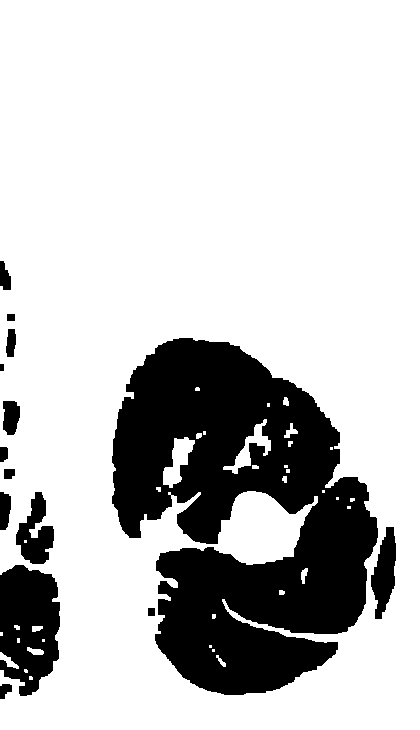
\includegraphics[height=7cm,trim=0 0 0 6cm, clip]{images/fiber_creation/extraction_segmentation_482.png}}\quad%
  \fcolorbox{black}{black}{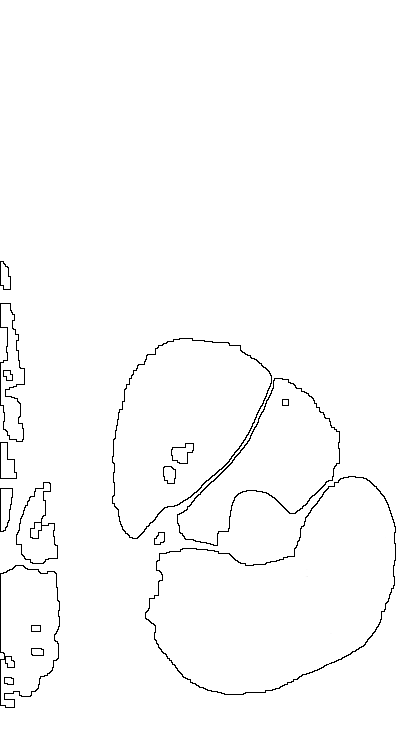
\includegraphics[height=7cm,trim=0 0 0 4cm, clip]{images/fiber_creation/extraction_contour_482.png}}\vspace*{5mm}\\
  \fcolorbox{black}{black}{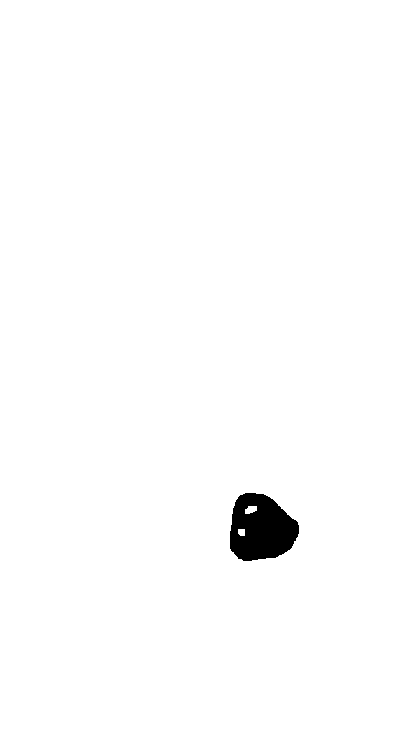
\includegraphics[height=7cm,trim=0 0 0 6cm, clip]{images/fiber_creation/extraction_bone482.png}}\quad%
  \fcolorbox{black}{black}{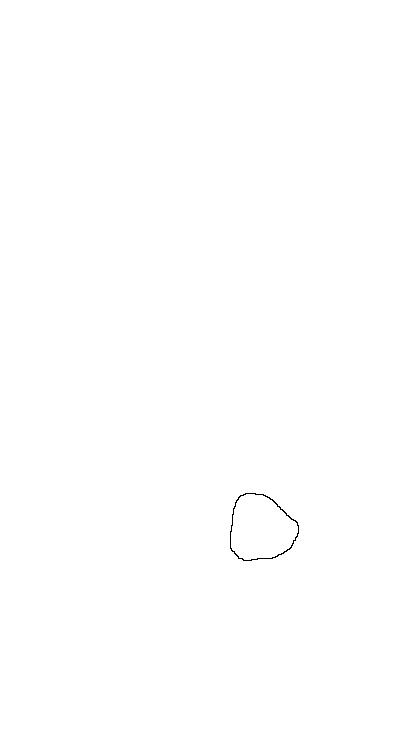
\includegraphics[height=7cm,trim=0 0 0 6cm, clip]{images/fiber_creation/extraction_surface_bone482.png}}%
  \caption{Intermediate steps of the algorithm to determine surface geometry of muscles and bones. The left columns shows pixels from the image in \cref{fig:vhp_image} that were categorized to be muscle tissue (top) and bone material (bottom). The right column shows a later step in the algorithm, where the surface of muscle (top) and bone (bottom) is estimated.}%
  \label{fig:extraction}%
\end{figure}%

In the next step, a single contour for each of muscle and bone is obtained in every image. If there are multiple contours per image, the one that is located closest to the upper right corner of the image is selected for the muscle. If all contours in an image are shorter than 20 pixels, this is an indication for bad segmentation quality and the whole image gets discarded. Because of the discarded images the resulting surface description has a lower resolution at the respective locations. This is not a problem as the data is subsequently approximated by a smooth spline surface.

The result is a set of contours for muscle and bone in the cross sectional planes of the images. Combining these, we get a point cloud in 3D space that approximates the surface of the biceps muscle and the surfaces of the considered bones humerus, ulna and radius. Using these points, a spline surface can be fitted and subsequently triangulated. Resulting surfaces for the biceps and humerus bones are shown in \cref{fig:extraction_result}.
%
\begin{figure}%
  \centering%
  \begin{subfigure}[t]{0.48\textwidth}%
    \centering%
    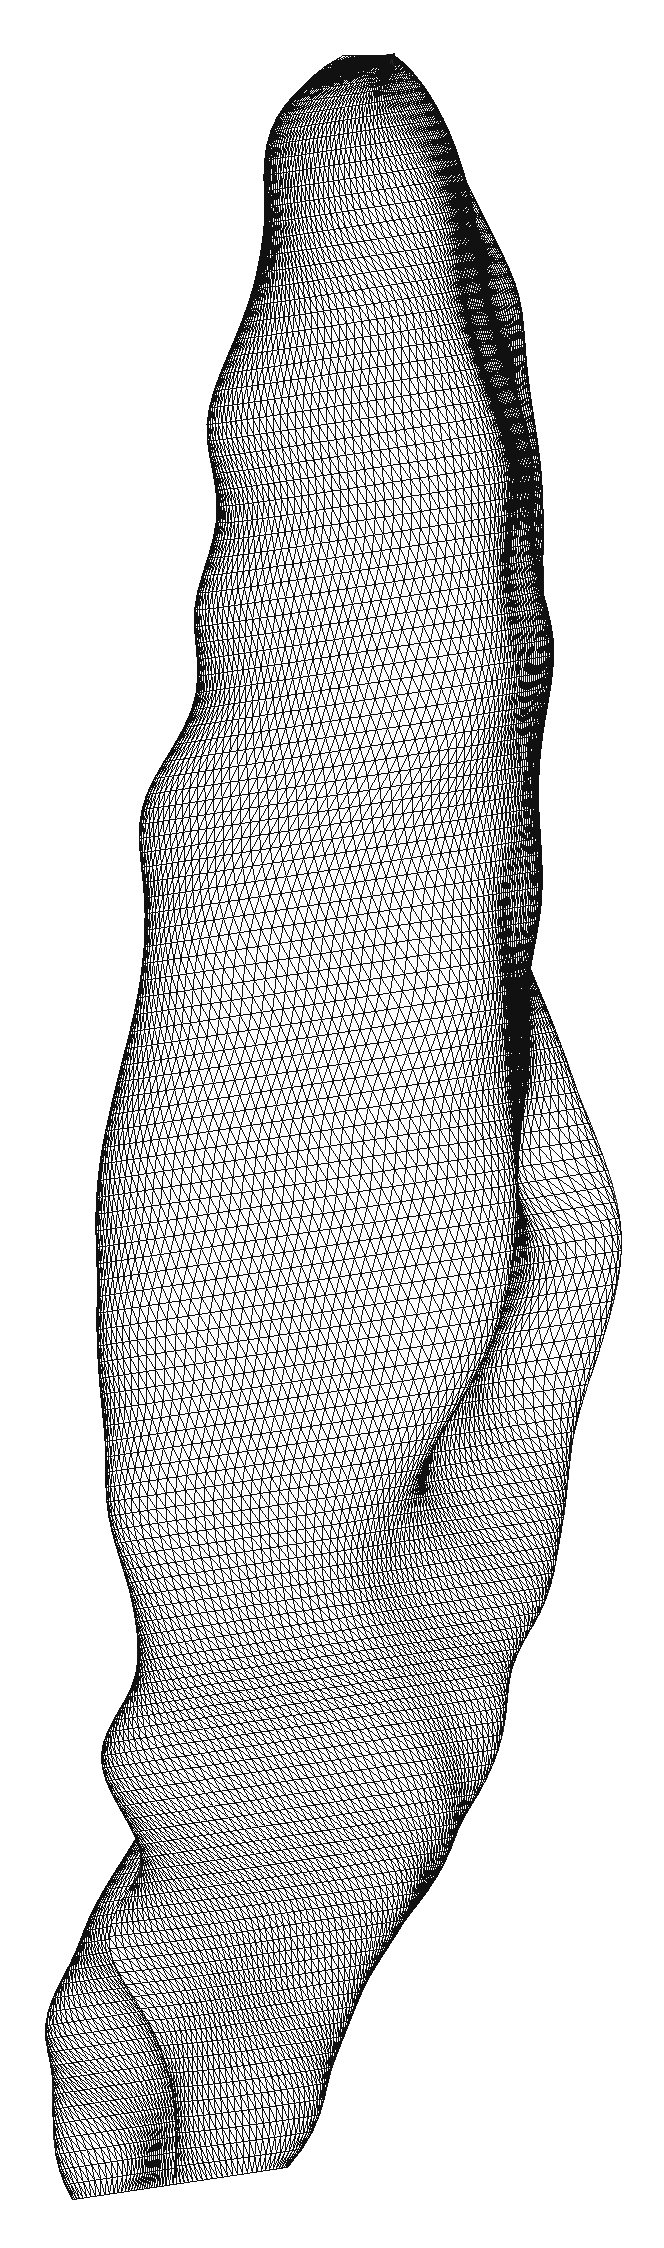
\includegraphics[height=7cm]{images/fiber_creation/extraction_biceps.png}%
    \caption{Surface of the biceps brachii muscle. At the right side of the muscle, the groove of the humerus bone can be seen.}%
    \label{fig:extraction_result_biceps}%
  \end{subfigure}
  \begin{subfigure}[t]{0.48\textwidth}%
    \centering%
    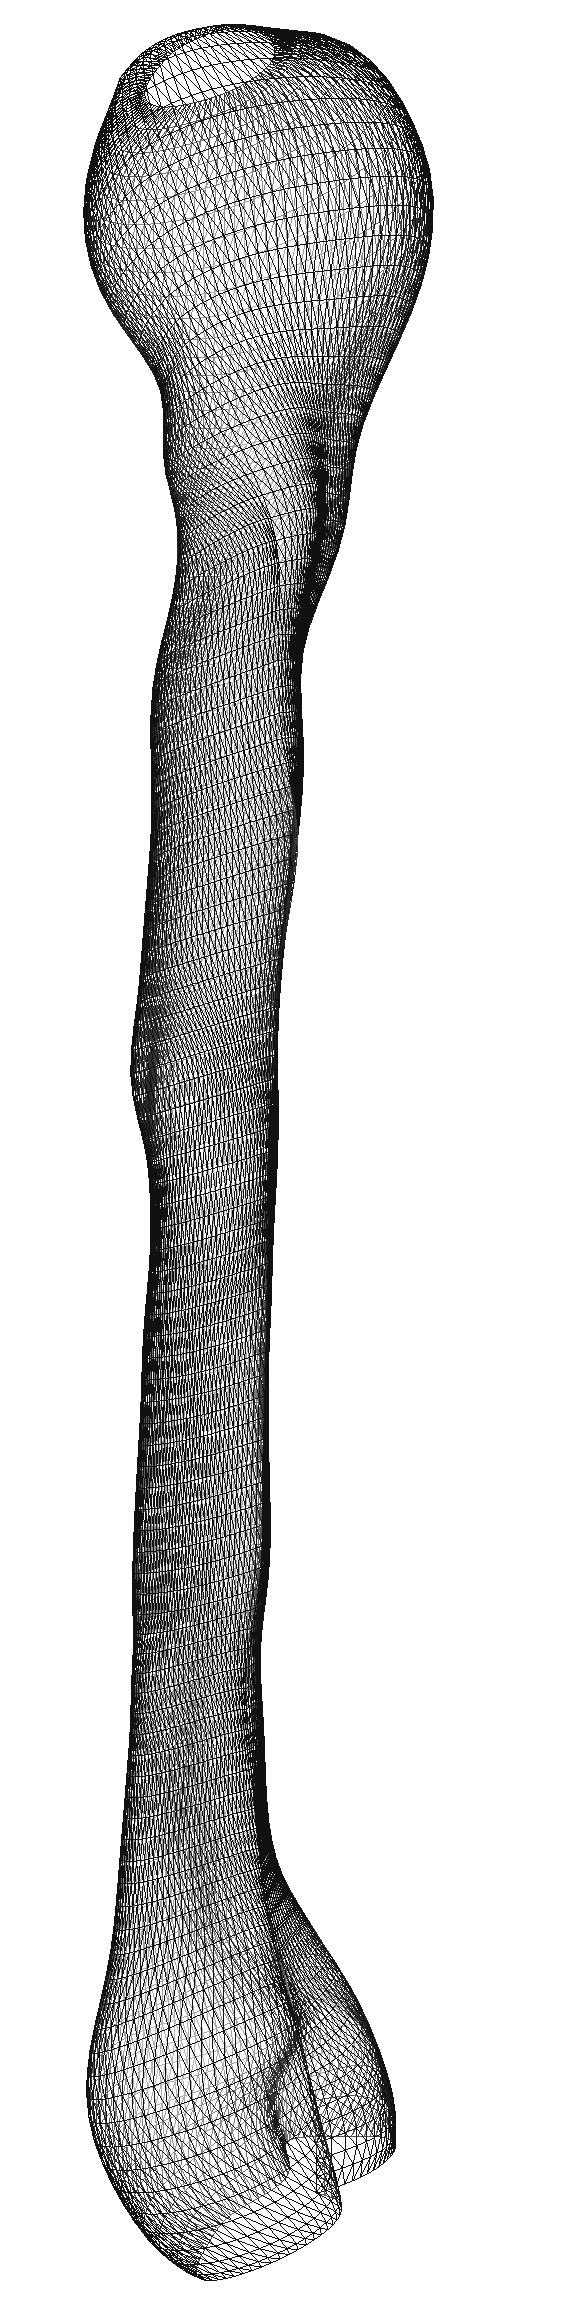
\includegraphics[height=7cm]{images/fiber_creation/extraction_humerus00.png}%
    \caption{Surface of the humerus.}%
    \label{fig:extraction_result_humerus}%
  \end{subfigure}    
  \caption{Surfaces of biceps and humerus bone obtained by the automatic surface extraction algorithm.}%
  \label{fig:extraction_result}%
\end{figure}%

The runtime for the algorithm applied on a dataset with \num{495} images and approximately \num{144e6} pixels in total was \SI{121}{\minute}. The used hardware was a AMD Ryzen 5 1600 processor with 6 cores, 3.2 GHz and \SI{16}{\giga\byte} RAM, of which a maximum of \SI{2}{\giga\byte} was used. Because processing of the images can be done in parallel, the runtime was reduced to approximately half (\SI{62}{\minute}) using 2 threads and to a quarter (\SI{30}{\minute}) using 6 threads.

The advantage of the presented algorithm is that the outcome solely depends on the imaging data and, thus, no modeling error by manual approximation of the geometry occurs. For example, the obtained surfaces of biceps and humerus geometrically fit perfectly into each other. Intermediate steps are stored as black and white images. By editing these between the steps of the algorithm, manual tweaking is possible and can be used to increase the quality of the results.

A disadvantage is that the algorithm relies on color information in the imaging data to differentiate between muscle and other tissue. Because some of the involved tissue types have similar colors, this approach can be error-prone. Furthermore, the color ranges need to be determined experimentally. Therefore, the algorithm is not very robust with respect to image noise and needs adjustments when it should be used to extract other muscles. Expert knowledge about the location and shape of human muscles cannot be used easily to improve the results of the algorithm.

An alternative approach is to manually segment the imaging data and construct surfaces with the help of a tool. This approach is described in the following section.

\subsection{Manually Guided Surface Extraction}\label{sec:surf_extr}

Manually guided segmentation can be done using the \emph{MAP client} of the Musculoskeletal Altas Project (MAP) \cite{mapclient}. This application allows to create and execute a workflow to achieve data processing and simulation tasks. In a graphical window, the user can place and connect various workflow steps. When executing the workflow, each step shows a dialog where the required configuration can be entered or the operations can be performed on a visual representation of the data at this workflow stage. 

Possible workflow steps include source and sink operations such as reading image data and writing meshes. Imaging data such as the 2D images from the Visual Human Male can be visualized in a 3D representation. The user can place points in the 3D space to mark boundaries of the visualized muscle and tissue structures.
Further workflow steps allow to create meshes of predefined geometrical shapes, such as cubes and cylinders and merge them into a common mesh. These meshes can be fitted to point clouds of user defined points. This is done by a least squares approach minimizing the distances between user created points and the mesh surface. Details can be found in \cite{Fernandez2018}.

The MAP client has a plugin architecture and allows to create new workflow steps. It imports features from OpenCMISS, especially data processing formats and tools from OpenCMISS Zinc. Meshes can be created with 3D cubic Hermite elements that allow for a high geometric modeling flexibility with a low number of nodes. Such meshes are stored in the OpenCMISS file format of \code{exnode} and \code{exelem} files.

As a result, meshes of individual muscles or the whole human organism can be created. \Cref{fig:vhp_geometry} shows meshes that were create from the cryosectioning data of the Visible Human Male. In \cref{fig:vhp_total}, almost the whole body has been extracted. In \cref{fig:vhp_detail}, the mesh consisting of cubic Hermite elements is visualized. A relatively coarse mesh width suffices to model a smooth surface of the body. When exported in the exfiles format from the MAP client, the data can be visualized, e.g., using \emph{cmgui}, the visualization tool of OpenCMISS Zinc.

\begin{figure}%
  \centering%  
  \begin{subfigure}[t]{0.48\textwidth}%
    \centering%
    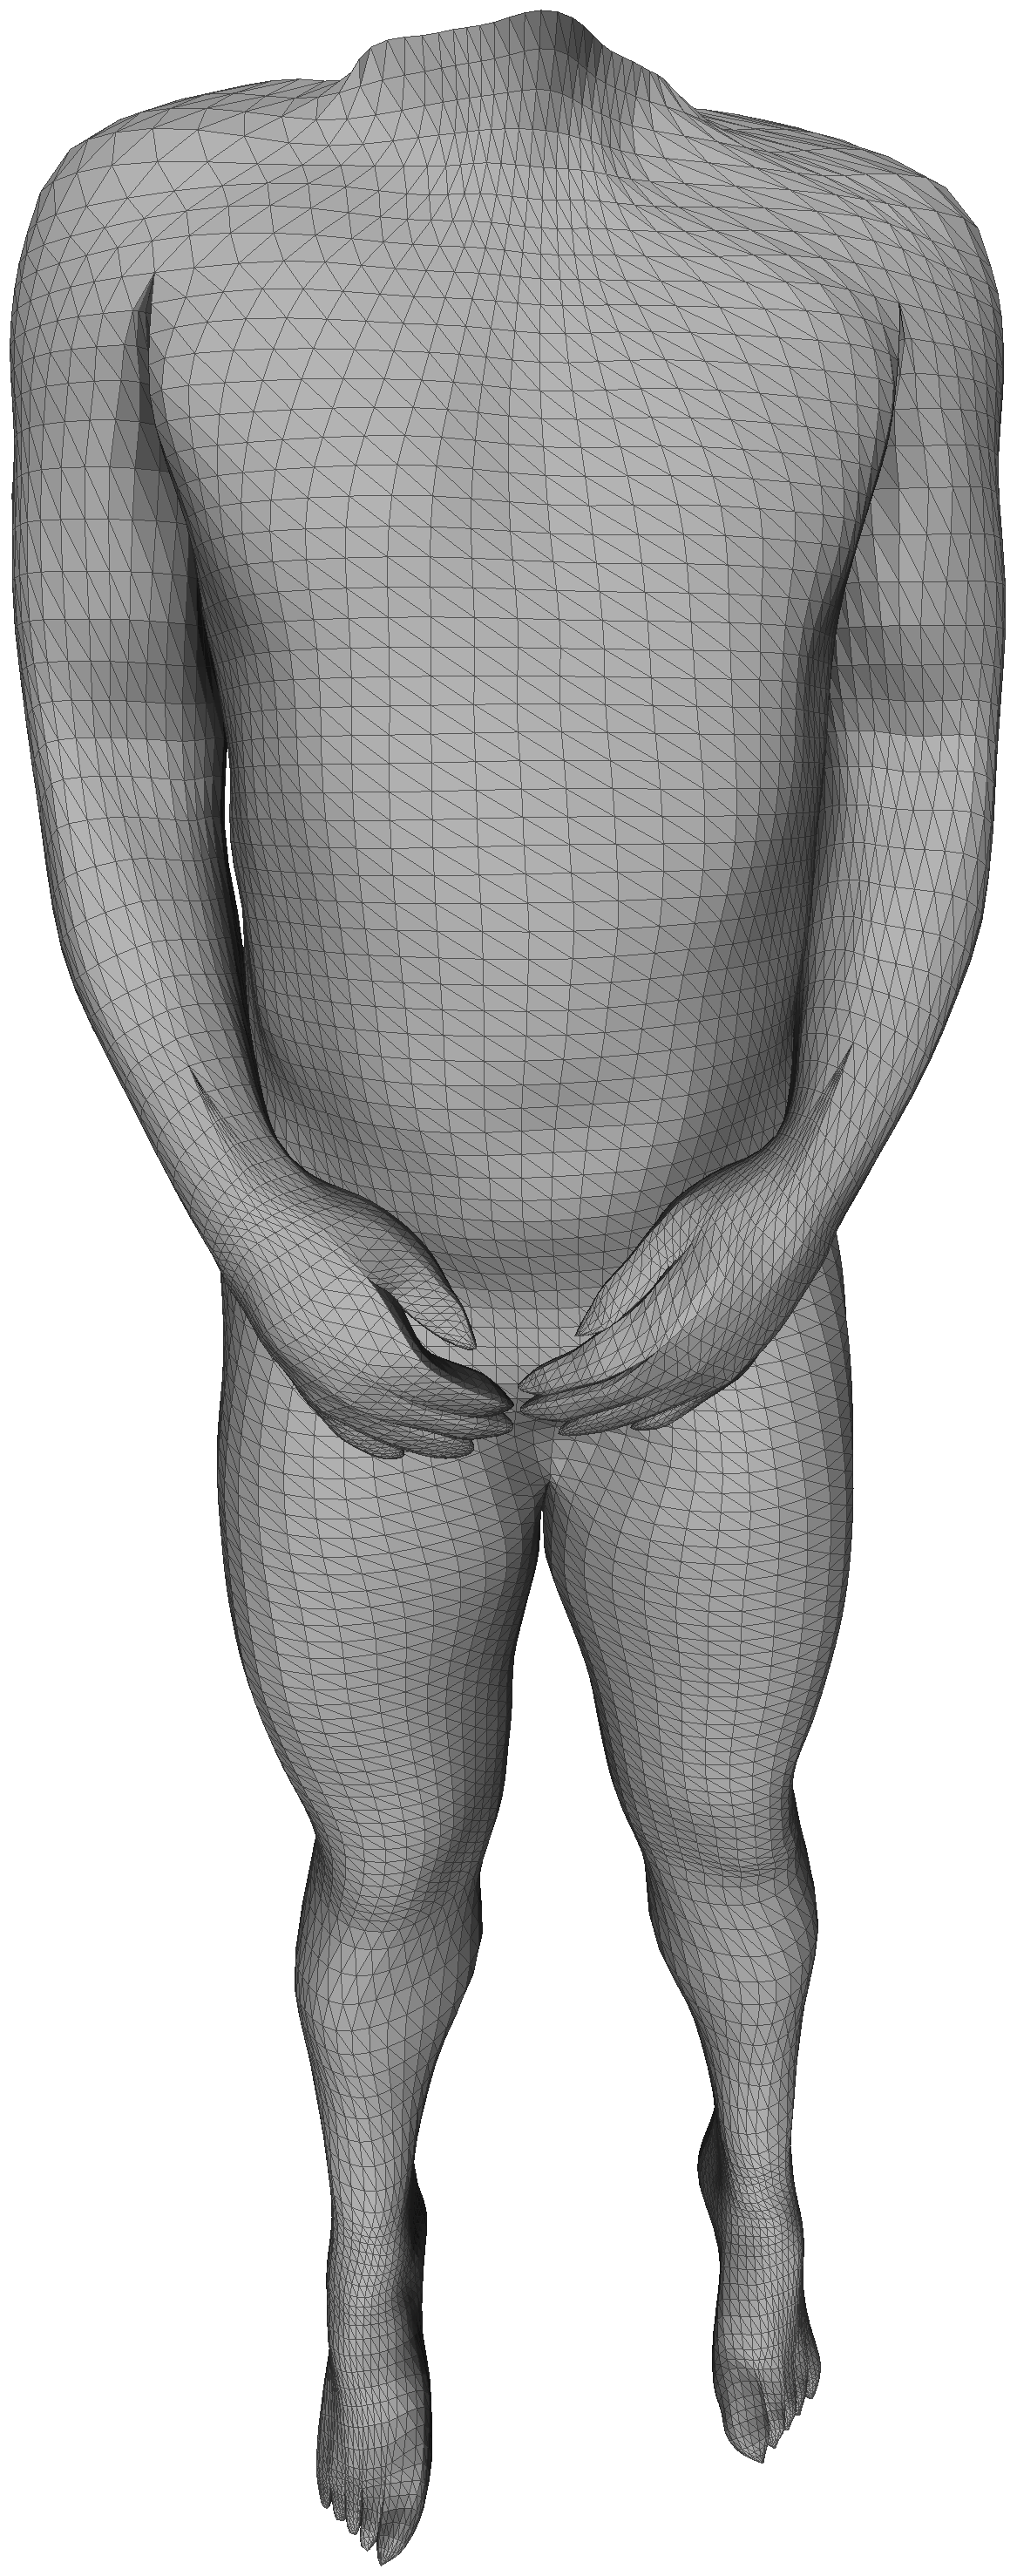
\includegraphics[height=10cm]{images/fiber_creation/skin00.png}%
    \caption{Mesh of the trunk and limbs, the surface has been triangulated for visualization.}%
    \label{fig:vhp_total}%
  \end{subfigure}
  \quad
  \begin{subfigure}[t]{0.48\textwidth}%
    \centering%
    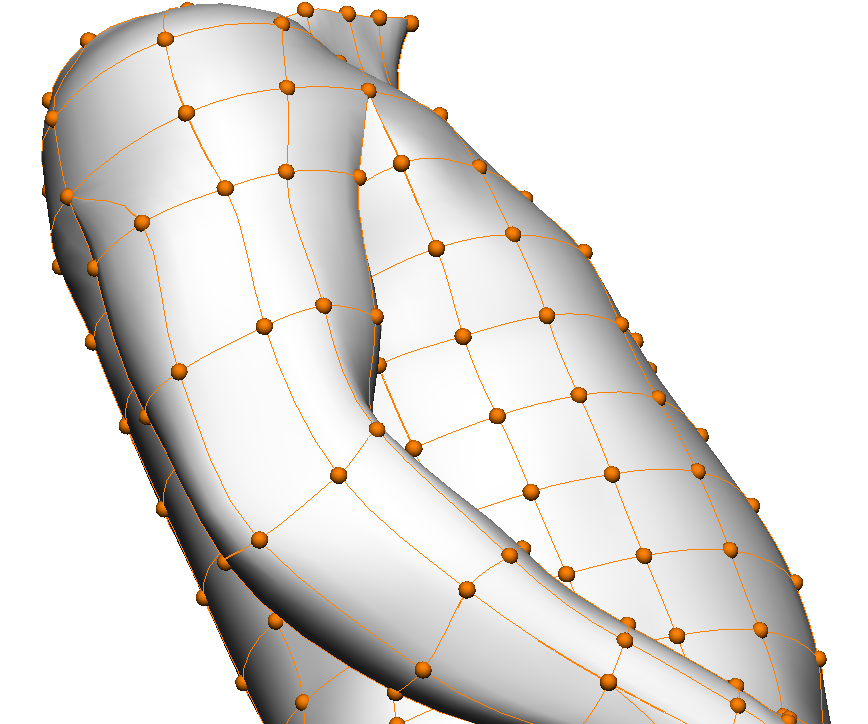
\includegraphics[height=7cm]{images/fiber_creation/elements4_red.png}%
    \caption{Detail view of part of the right upper arm and the trunk with orange nodes and edges of a cubic Hermite element mesh.}%
    \label{fig:vhp_detail}%
  \end{subfigure} 
  \caption{Mesh of the Visible Human Male from the Visible Human Project.}%
  \label{fig:vhp_geometry}% 
\end{figure}%

The mesh width of the meshes obtained using the MAP client was chosen such that the surface fitting yielded good results. The meshes are not necessarily ready for use in a simulation, especially if a  high mesh resolution is desired. 
Apart from the mesh width also the type of elements can be different than what is needed for a finite element simulation. Our goal is to obtain meshes with linear or quadratic Lagrange elements with configurable mesh widths for the specified upper arm muscles, such as the biceps brachii.

Therefore, the next step of the workflow, as visualized by the right branch of \cref{fig:scheme_preprocessing}, is to transform the volume mesh into a surface mesh which then can be used as start for further meshing. The further meshing steps are visualized in \cref{fig:biceps_processing}. The start is the Hermite mesh shown in the left-most image.

\begin{figure}%
  \centering%
  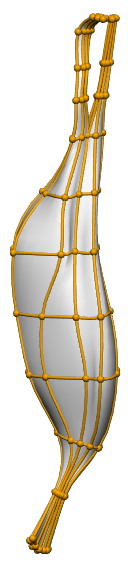
\includegraphics[height=10cm]{images/fiber_creation/exfile_red.png}\quad%
  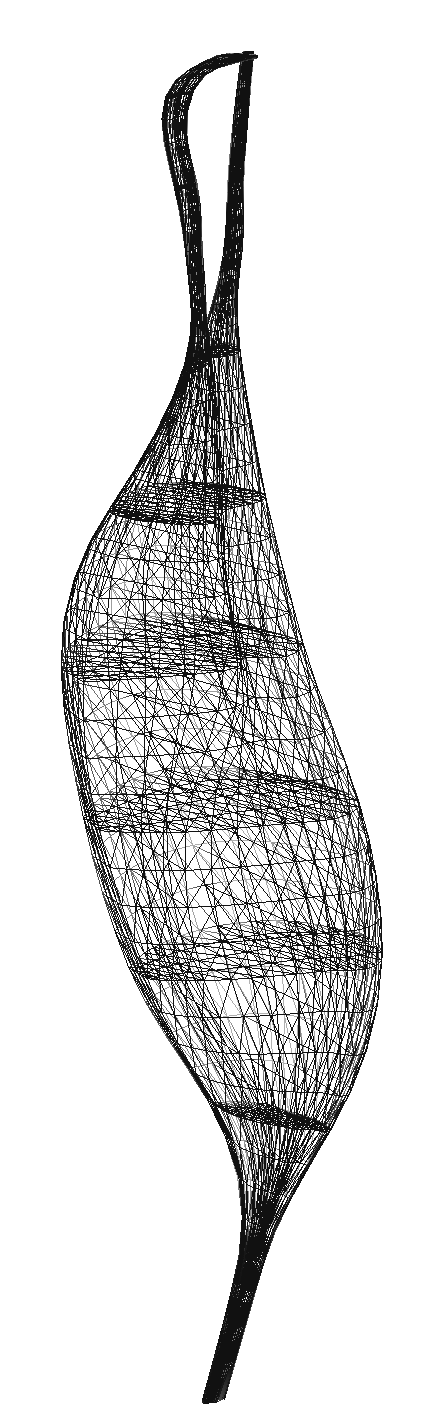
\includegraphics[height=10cm]{images/fiber_creation/biceps23.png}%
  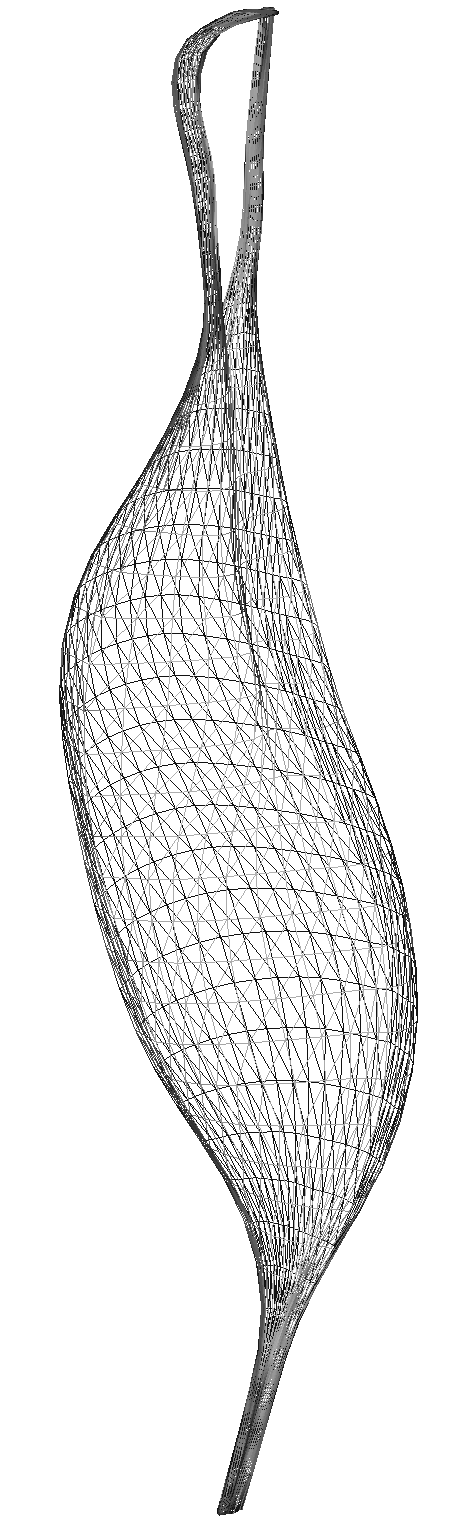
\includegraphics[height=10cm]{images/fiber_creation/biceps22.png}%
  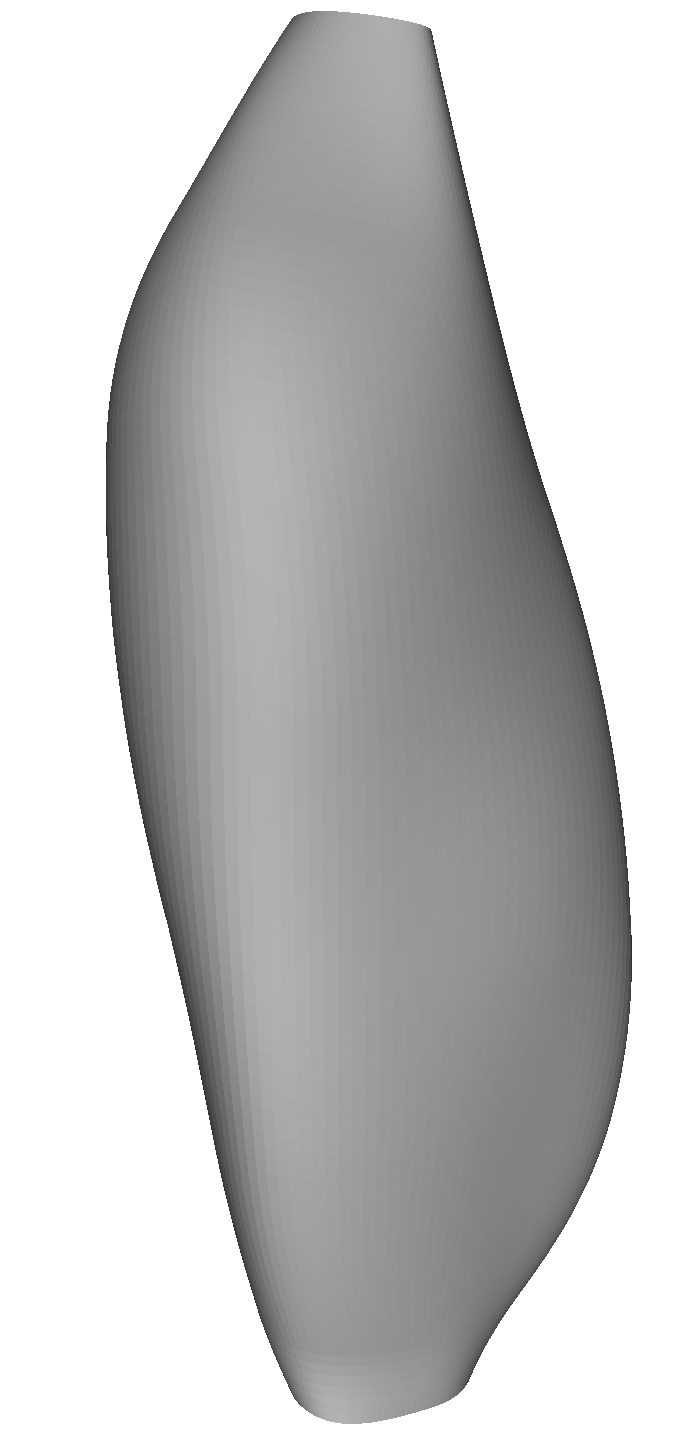
\includegraphics[height=10cm,trim=-2cm 0 0 -2cm, clip]{images/fiber_creation/splines00.png}%
  \caption{Processing the geometry of the biceps brachii muscle. From left to right: mesh with cubic Hermite elements, STL mesh with inside triangles, STL surface mesh where triangles lying inside have been removed, Spline surface of the muscle belly.}%
  \label{fig:biceps_processing}%
\end{figure}%

The Hermite elements can be triangulated and stored as an STL file using the tool \mbox{\code{cmgui}.} This process triangulates the non-planar faces of all Hermite elements. This leads to a dataset with triangles both on the surface and in the inside of the volume, as can be seen in the second image of \cref{fig:biceps_processing}. At this stage, the use of the MAP and OpenCMISS related tools is finished and further processing steps are performed using tools from \opendihu{} that we developed on our own.

A Python script removes the triangles inside the volume. The detection whether a triangle is inside the volume is done by casting four rays from the center of gravity of the respective triangle and determining if the rays intersect any other triangles. The rays have directions $(x,y,z) = (\pm1,\pm1,\frac13)$, where the $z$ axis is oriented along the muscle's longitudinal axis and the $x$ and $y$ axes are oriented in radial direction. The ray-triangle intersection is done using the fast Möller-Trumbore algorithm \cite{ray-triangle}. For every ray, all triangles are checked.
Only if all four rays intersect at least one more triangle, the starting triangle is considered to be inside the volume and subsequently removed from the dataset. 

This algorithm has a quadratic time complexity $\O(n^2)$ in the number of triangles $n$. It could be improved by organizing the triangles in a spatially adaptive data structure, such as an octree. However, since this preprocessing step has to be performed only once for a given geometry, the runtime is not critical and there is no need for such optimization.

The result of this operation is a triangulated surface, shown in the third image of \cref{fig:scheme_preprocessing}. The next step is to create a Spline surface of the muscle belly, as shown in the right-most image of \cref{fig:scheme_preprocessing}. This is described in the next two sections.

\subsection{Introduction of Spline Surfaces}\label{sec:nurbs}
After the surface representation of the muscle has been obtained from either the left or the right branch of the preprocessing workflow in \cref{fig:scheme_preprocessing}, the surface is given by a point cloud or a number of triangles. To remedy eventual outliers or unphysiological sharp edges from the segmentation, a Spline surface is fitted to the data. This leads to a smooth surface representation and later to a better conditioned finite element mesh in the simulation. However, this step is optional. It is also possible to directly use the surface triangulation from \cref{sec:surf_extr} for the meshing algorithm described in \cref{sec:ser_alg_meshes}.

The surfaces use Nonuniform Rational B-splines (NURBS). A NURBS surface is a generalization of a B-spline surface. From a modeling point of view, B-spline surfaces have three advantageous properties.
First, the B-spline surface can be constructed with given smoothness properties.  
Second, the definition of a particular B-spline surface builds on intuitive geometric information, which simplifies their creation: A control polygon mesh in 3D space is defined. Its convex hull is guaranteed to contain the surface.
Third, the geometric parameters of a B-spline surface have only local impact on the shape of the surface. This allows a B-spline surface of a fixed, low polynomial degree to approximate point clouds with any number of points without loosing approximation quality.

A limitation of B-spline surfaces is that circular and spherical shapes cannot be represented. This limitation is overcome by NURBS surfaces. NURBS surfaces are defined as the perspective projection into 3D space of a B-spline surface in 4D space.

The mathematical description is given in this section, following the notation of \cite{piegl2012nurbs}. The building blocks are the B-spline basis functions of polynomial degree $p$. Given a knot vector 
%
\begin{align*}
  \Xi = (\xi_1, \xi_2, \dots, \xi_k) \in \R^k \quad \text{with } a=\xi_1 \leq \xi_2 \leq \cdots \leq \xi_k = b,
\end{align*}
%
the $i$th B-spline basis function $N_{i,n}$ of degree $n$ is defined recursively starting with the piecewise constant function
%
\begin{align*}
  N_{i,0}(\xi) = \begin{cases} 
    1 \, &\text{for }\xi_i \leq \xi < \xi_{i+1},\\[2mm]
    0 &\text{else},
  \end{cases}
\end{align*}
and using the following relation to define the functions of higher degree $(n > 0)$:
\begin{align*}
  N_{i,n}(\xi) = \dfrac{\xi - \xi_i}{\xi_{i+n} - \xi_i} N_{i,n-1}(\xi) + \dfrac{\xi_{i+n+1} - \xi}{\xi_{i+n+1} - \xi_{i+1}} N_{i+1,n-1}(\xi), \quad \text{for all }i > 0.
\end{align*}
Because neighboring entries in the knot vector can be equal, the fraction $0/0$ can occur. In this case, $0/0 := 0$ is defined. Note that by construction of $N_{i,n}$ a zero denominator implies that also the dividend is zero.

A B-spline curve $\bfC: \R \to \R^d$ of polynomial degree $p$ is defined as
%
\begin{align*}
  \bfC(u) = \s{i=1}{l}N_{i,p}(u)\,\bfP_i, \quad u \in [a,b].
\end{align*}
%
The coefficients $\bfP_i \in \R^d, i=1, \dots, l$, of the basis functions $N_{i,p}$ are called \emph{control points} and define the control polygon. The number $l$ of basis functions and control points is determined from the number of knots $k$ in an open knot vector and the polynomial degree $p$ as $l = k-p-1$.

The number of equal entries in series in the knot vector is the \emph{multiplicity} of the respective knot value. Usually \emph{open} knot vectors $\Xi$ are used where the first and the last knot occur with a multiplicity of $p+1$.
This makes the first and the last points of the B-spline curve coincide with the control polygon points: $\bfC(a) = \bfP_1$ and $\bfC(b) = \bfP_l$.

The multiplicities of the knots in the knot vector encode information about the smoothness of the B-spline curve. If the knot value $\hat{\xi}$ has a multiplicity of $m$, the B-spline curve will be $(p-m)$ times continuously differentiable at $\bfC(\hat{\xi})$.
% This can be seen from the fact that there exist $m$ basis functions with a support that begins at $\hat{\xi}$.

An exemplary B-spline curve is shown in \cref{fig:bspline_curve}. It uses a \emph{non-uniform} knot vector for polynomial degree $p=3$, where the differences $\xi_{i+m} - \xi_i$ between neighboring knot values vary. The effect of different multiplicities can be seen. The multiplicity $m=p=3$ places the point of the curve at the knot on the respective control point, as for $\xi=49$ in the example. The multiplicity $m=p-1=2$ places the point of the curve at the knot on the control polygon, as in the example at $\xi=10$. A lower multiplicity $m < p-1$ does not yield a higher smoothness and in turn does not force the curve to coincide with the control polygon at the respective knot. It can also be seen that the B-spline curve stays inside the convex hull of the control polygon which is a property of B-spline curves \cite{piegl2012nurbs}.

\begin{figure}%
  \centering%
  \def\svgwidth{8cm}%
  \input{images/fiber_creation/bspline_curve.pdf_tex}%
  \caption{Exemplary B-spline curve (red) of degree $p=3$ for the knot vector $\Xi = (0,0,0,0,7,10,10,49,49,49,50,50,50,50)$, control points (blue) and control polygon (black).
  Positions of the curve $\bfC(\xi_i)$ at the knots $\xi_i$ are indicated by the red squares and the knot value $\xi$ and its multiplicity $m$ is given. The effect of moving one control point is shown in green.}%
  \label{fig:bspline_curve}%
\end{figure}%
%
The effect of moving one of the 10 control points is visualized with green color in \cref{fig:bspline_curve}.
The B-spline basis function $N_{i,p}$ has a local support of $S=(\xi_i,\xi_{i+p+1})$. Consequently, only the corresponding part of the curve, $\bfC(\xi)$ for $\xi \in S$, changes.

A B-spline surface $\bfS : \R^2 \to \R^d$ is given by the tensor product of two B-spline curves:
\begin{equation}\label{eq:bspline_surface}
  \begin{array}{lll}
    \bfS(u,v) = \s{i=1}{l^{(1)}}\s{j=1}{l^{(2)}} N^{(1)}_{i,p^{(1)}}(u)\,N^{(2)}_{j,p^{(2)}}(v)\, \bfP_{i,j}.
  \end{array}
\end{equation}

Here, we have two polynomial degrees $p^{(1)}$ and $p^{(2)}$, the ansatz functions $N^{(1)}_{i,p^{(1)}}$ and $N^{(2)}_{j,p^{(2)}}$ with $l^{(1)}$ and $l^{(2)}$ ansatz functions per coordinate direction are constructed from the corresponding knot vectors per coordinate direction.

NURBS, B-spline curves and surfaces are formulated using \emph{homogeneous coordinates}. Every point in Cartesian coordinates $(x,y,z) \in \R^3$ has a set of homogeneous coordinates $(\tilde{x},\tilde{y},\tilde{z},w)=(x\,w,y\,w,z\,w,w)$. Thus, the Cartesian coordinates can be obtain from the homogeneous coordinates by the \emph{perspective division}, i.e., dividing all but the last coordinate by the weight $w$.

A NURBS surface is given by the same definition as the B-spline surface in \cref{eq:bspline_surface} except that the control points $\bfP_{i,j} \in \R^3$ are enriched with scalar weights $w_{i,j}$ and, thus, replaced by $(\bfP_{i,j}, w_{i,j}) \in \R^4$. The resulting surface $\bfS$ is given in homogeneous coordinates. Executing the perspective division yields the form:
%
\begin{align*}
  &\bfT(u,v) = \s{i=1}{l^{(1)}}\s{j=1}{l^{(2)}} R_{i,j}(u,v) \,\bfP_{i,j},\\[4mm]
  &\text{with } R_{i,j}(u,v) = \dfrac{N_{i,p^{(1)}}(u)\,N_{j,p^{(2)}}(v)\,w_{i,j}}{\s{r=1}{l^{(1)}}\s{s=1}{l^{(2)}} N_{r,p^{(1)}}(u)\,N_{s,p^{(2)}}(v)\,w_{r,s}}.
\end{align*}
The new rational basis functions $R_{i,j}$ and the possibly non-uniform knot vectors give rise to the name Non-Uniform Rational B-spline surface (NURBS).

\subsection{Fitting a Spline Surface to the Muscle Geometry}
In order to find a NURBS surface for the given triangulated surface of a muscle, at first, the part of the geometry corresponding to the tendons is removed such that the resulting triangles model only the surface of the muscle belly. In our example of the biceps muscle, the resulting belly has a length of \SI{12.8}{\mm}.

Then, twelve cross sections are extracted from the surface triangles. As a result, we get twelve horizontal circumferential rings. On each ring, 9 equidistant points are determined. The first point is appended after the last point in every ring, such that in total we obtain a grid of $10 \times 12$ points. 

Then, the least squares surface approximation algorithm by \cite{piegl2012nurbs} is used to fit a NURBS surface to the points. The implementation of the algorithm is given by the NURBS-Python (geomdl) library. Polynomial degrees of $p^{(1)} = 3$ and $p^{(2)}=2$ are used where the first dimension corresponds to the cross sectional direction of the muscle. The knot multiplicity is chosen as $m=1$ for both coordinate directions. We obtain a two times respective one times continuously differentiable surface in $u$ and $v$ direction. 
The resulting NURBS surface and the control polygon are visualized in \cref{fig:biceps_splines_control_points}. Note that the control polygon is different from the grid of points against which the surface is fitted.
%
\begin{figure}%
  \centering%
  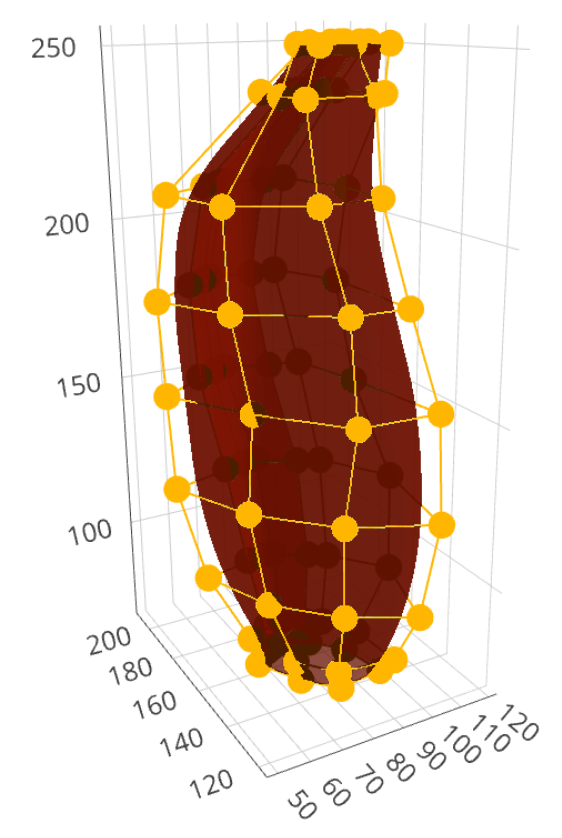
\includegraphics[width=0.35\textwidth]{images/fiber_creation/splines01red.png}%
  \caption{Muscle surface description with Splines: Fitted NURBS surface of the biceps muscle (red) and the control polygon (orange).}%
  \label{fig:biceps_splines_control_points}%
\end{figure}%

\Cref{fig:biceps_splines_wrong} shows the result of this approach in more detail. We observe that the surface is non-differentiable and has a kink at the seam line where the first and last points of each ring meet. The reason for this is that the surface fitting algorithm does not pose any conditions on the tangents at the edges of the fitted NURBS surface.  Thus, the tangents mismatch.

Since no implementation of a fitting algorithm specifically for a tubular NURBS surface with periodicity in tangential direction is available, we develop a different remedy. We modify the point grid that is used for the surface fitting. The series of 9 equidistant points on each ring is replicated twice and the first point is again added as the last point. This leads to a grid of $(3\cdot 9+1) = 28 \times 12$ points which wrap around the muscle volume in cirumferential direction three times. The NURBS surface fitting algorithm is applied on this grid. The resulting NURBS surface also wraps around the muscle three times with the two ends being again not properly fitting to each other. From these three wraps, the middle one is extracted. In the biceps example, this corresponds to restricting the NURBS surface $\bfT(u,v)$ from $(u,v) \in [0,1]^2$ to $(u,v) \in [0.4,0.733]\times [0,1]$.

The result is depicted in \cref{fig:biceps_splines_seam}. The tangents now match very well between the two sides of the NURBS surface. Additionally, the comparison with the inital approach in \cref{fig:biceps_splines_wrong} shows that an artificial bulge at the top of the muscle in the perspective of the visualization is removed. The overall shape of the muscle now looks smoother and more natural. Also, a comparison with the result of the automatic algorithm given in \cref{fig:extraction_result_biceps} shows that the results of our new approach are smoother.

The generated tubular surface has two holes at the top and bottom which prevent it from being an enclosing surface to the muscle belly volume. The borders of these holes each lie in a plane and, thus, the missing surfaces are treated as being planar during the subsequent creation of the 3D meshes.

For the next step, a triangulation of the tubular surface is created and stored as STL mesh file. We use the respective functionality of the NURBS-Python library that creates a structured triangle mesh using the 2D parametrization of the NURBS surface.

%
\begin{figure}%
  \centering%
  \begin{subfigure}[t]{0.48\textwidth}%
    \centering%
    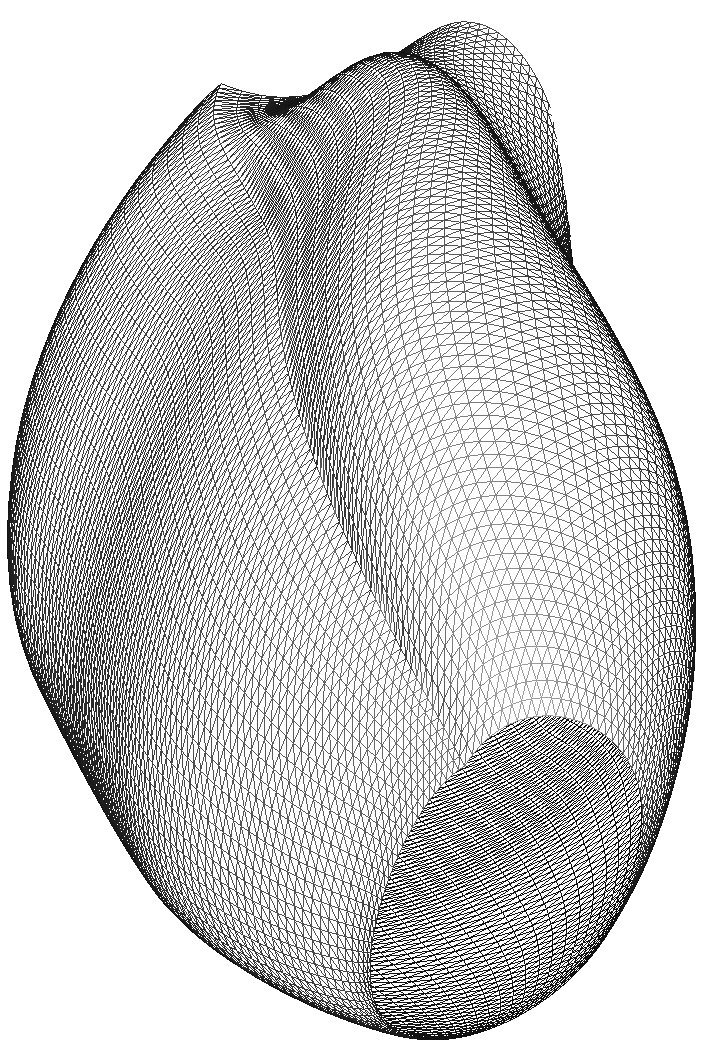
\includegraphics[height=8cm]{images/fiber_creation/splines_wrong00.png}%
    \caption{First approach with $10 \times 12$ control points. The kink at the seam line along the muscle is clearly visible.}%
    \label{fig:biceps_splines_wrong}%
  \end{subfigure}
  \quad
  \begin{subfigure}[t]{0.48\textwidth}%
    \centering%
    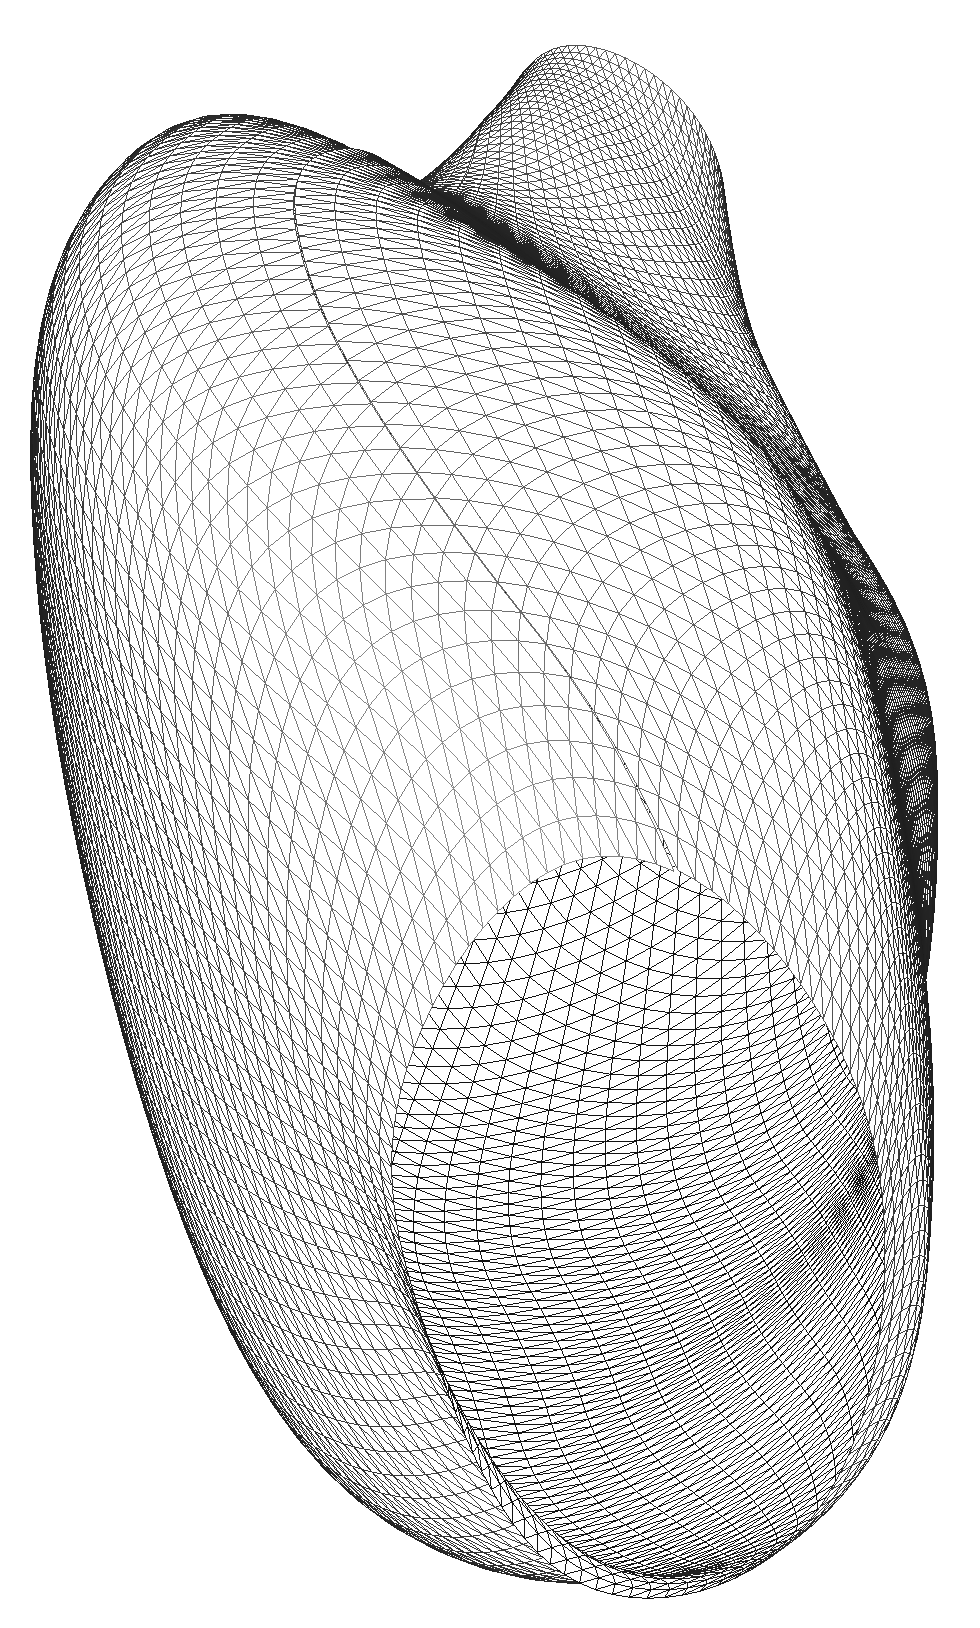
\includegraphics[height=8cm]{images/fiber_creation/splines_seam00.png}%
    \caption{Second, improved approach with $28 \times 12$ points. It can be seen that the tangents at the seam line match very well.}%
    \label{fig:biceps_splines_seam}%
  \end{subfigure}
  \caption{Muscle surface description with Splines: Fitted NURBS surface of the biceps muscle, triangulated for visualization purposes.}%
  \label{fig:biceps_splines}%
\end{figure}%
%
\section{Serial Algorithm to Create Muscle and Fiber Meshes}\label{sec:ser_alg_meshes}
Next, a 3D mesh for the muscle volume and 1D meshes for muscle fibers need to be generated from the surface representation described in the previous sections. In this section, first an algorithm for the 3D mesh is described. Then, a second algorithm that reuses results from the first algorithm is presented which generates one dimensional meshes for muscle fibers. Both algorithms are executed in serial. A derived algorithm that can run in parallel and, thus, can handle larger datasets on a distributed memory hardware is presented in \cref{sec:parallel_algorithm}.

The steps of a serial algorithm for the generation of a 3D mesh are given in \cref{alg:serial_algorithm_1}. Input is the set of triangles at the tubular surface of the muscle. The tubular surface is oriented along the $z$ axis. In the following descriptions, the muscle in considered to be oriented upright such that the $z$ axis points in vertical direction towards the top. The borders at the bottom and at the top have a constant $z$ coordinate.
%
\begin{algorithm}
  \begin{algorithmic}[1]%
    \Procedure{Create\_3D\_mesh}{}
    \Require Triangulated tubular surface
    \Ensure Structured 3D volume mesh
    \Statex
    \State Slice geometry           \label{alg:1.1}
    \State Triangulate 2D slices      \label{alg:1.2}
    \State Compute harmonic maps $u, v$ from the slices to a parameter space     \label{alg:1.3}
    \State Construct regular grid in parameter space and map it to slices            \label{alg:1.4}
    \State Form 3D quadrilateral elements between the 2D slices’ meshes   \label{alg:1.5}
    \EndProcedure
  \end{algorithmic}%
  \caption{Serial algorithm for generation of 3D meshes}%
  \label{alg:serial_algorithm_1}%
\end{algorithm}%

The idea of the algorithm is to first create 2D meshes with good quality on cross sectional slices of the muscle volume and then combine them to get a 3D mesh. The algorithm starts with creating the horizontal 2D slices in lines \ref{alg:1.1} and \ref{alg:1.2}. The slices get vertically connected at the end of the algorithm in line \ref{alg:1.5} to create the 3D mesh. This step is visualized in \cref{fig:serial_alg_8}. 

Because the goal is to create a hexahedral mesh, the horizontal slices have to consist of quadrilaterals. 
Decomposing a 2D domain into quadrilaterals is easier for a square or circular shaped domain than for an actual cross section of the muscle. Therefore, we introduce a separate, square or circular shaped parameter domain for creating the quadrilaterals.

\Cref{fig:harmonic_map_solution} outlines the method.
We start at the upper left of the figure with a triangulation on the cross sectional slices of the muscle. A mapping from the muscle slices to the parameter space at the right of the figure is computed. We use harmonic maps to ensure a smooth mapping that results in good mesh quality. This first steps corresponds to line \ref{alg:1.3} in \cref{alg:serial_algorithm_1}. Different parameter domains such as unit circle and unit square are considered, as shown in \cref{fig:harmonic_map_solution}. It can also be seen at the upper right that the image of the muscle slice triangulation in the parameter domain is better in the unit circle than in the unit square. Therefore, an investigation of different parameter domains and triangulation schemes is necessary.

Next, line \ref{alg:1.4} of \cref{alg:serial_algorithm_1} defines a quadrangulation in the parameter space, shown at the lower right of \cref{fig:harmonic_map_solution}. The quadrilateral elements are mapped back to muscle slices where they are needed for the final 3D mesh. An optional smoothing step at the lower left of the figure further improves the mesh quality.
All steps of the algorithm are described in more detail in the following sections.

\begin{figure}%
  \centering%
  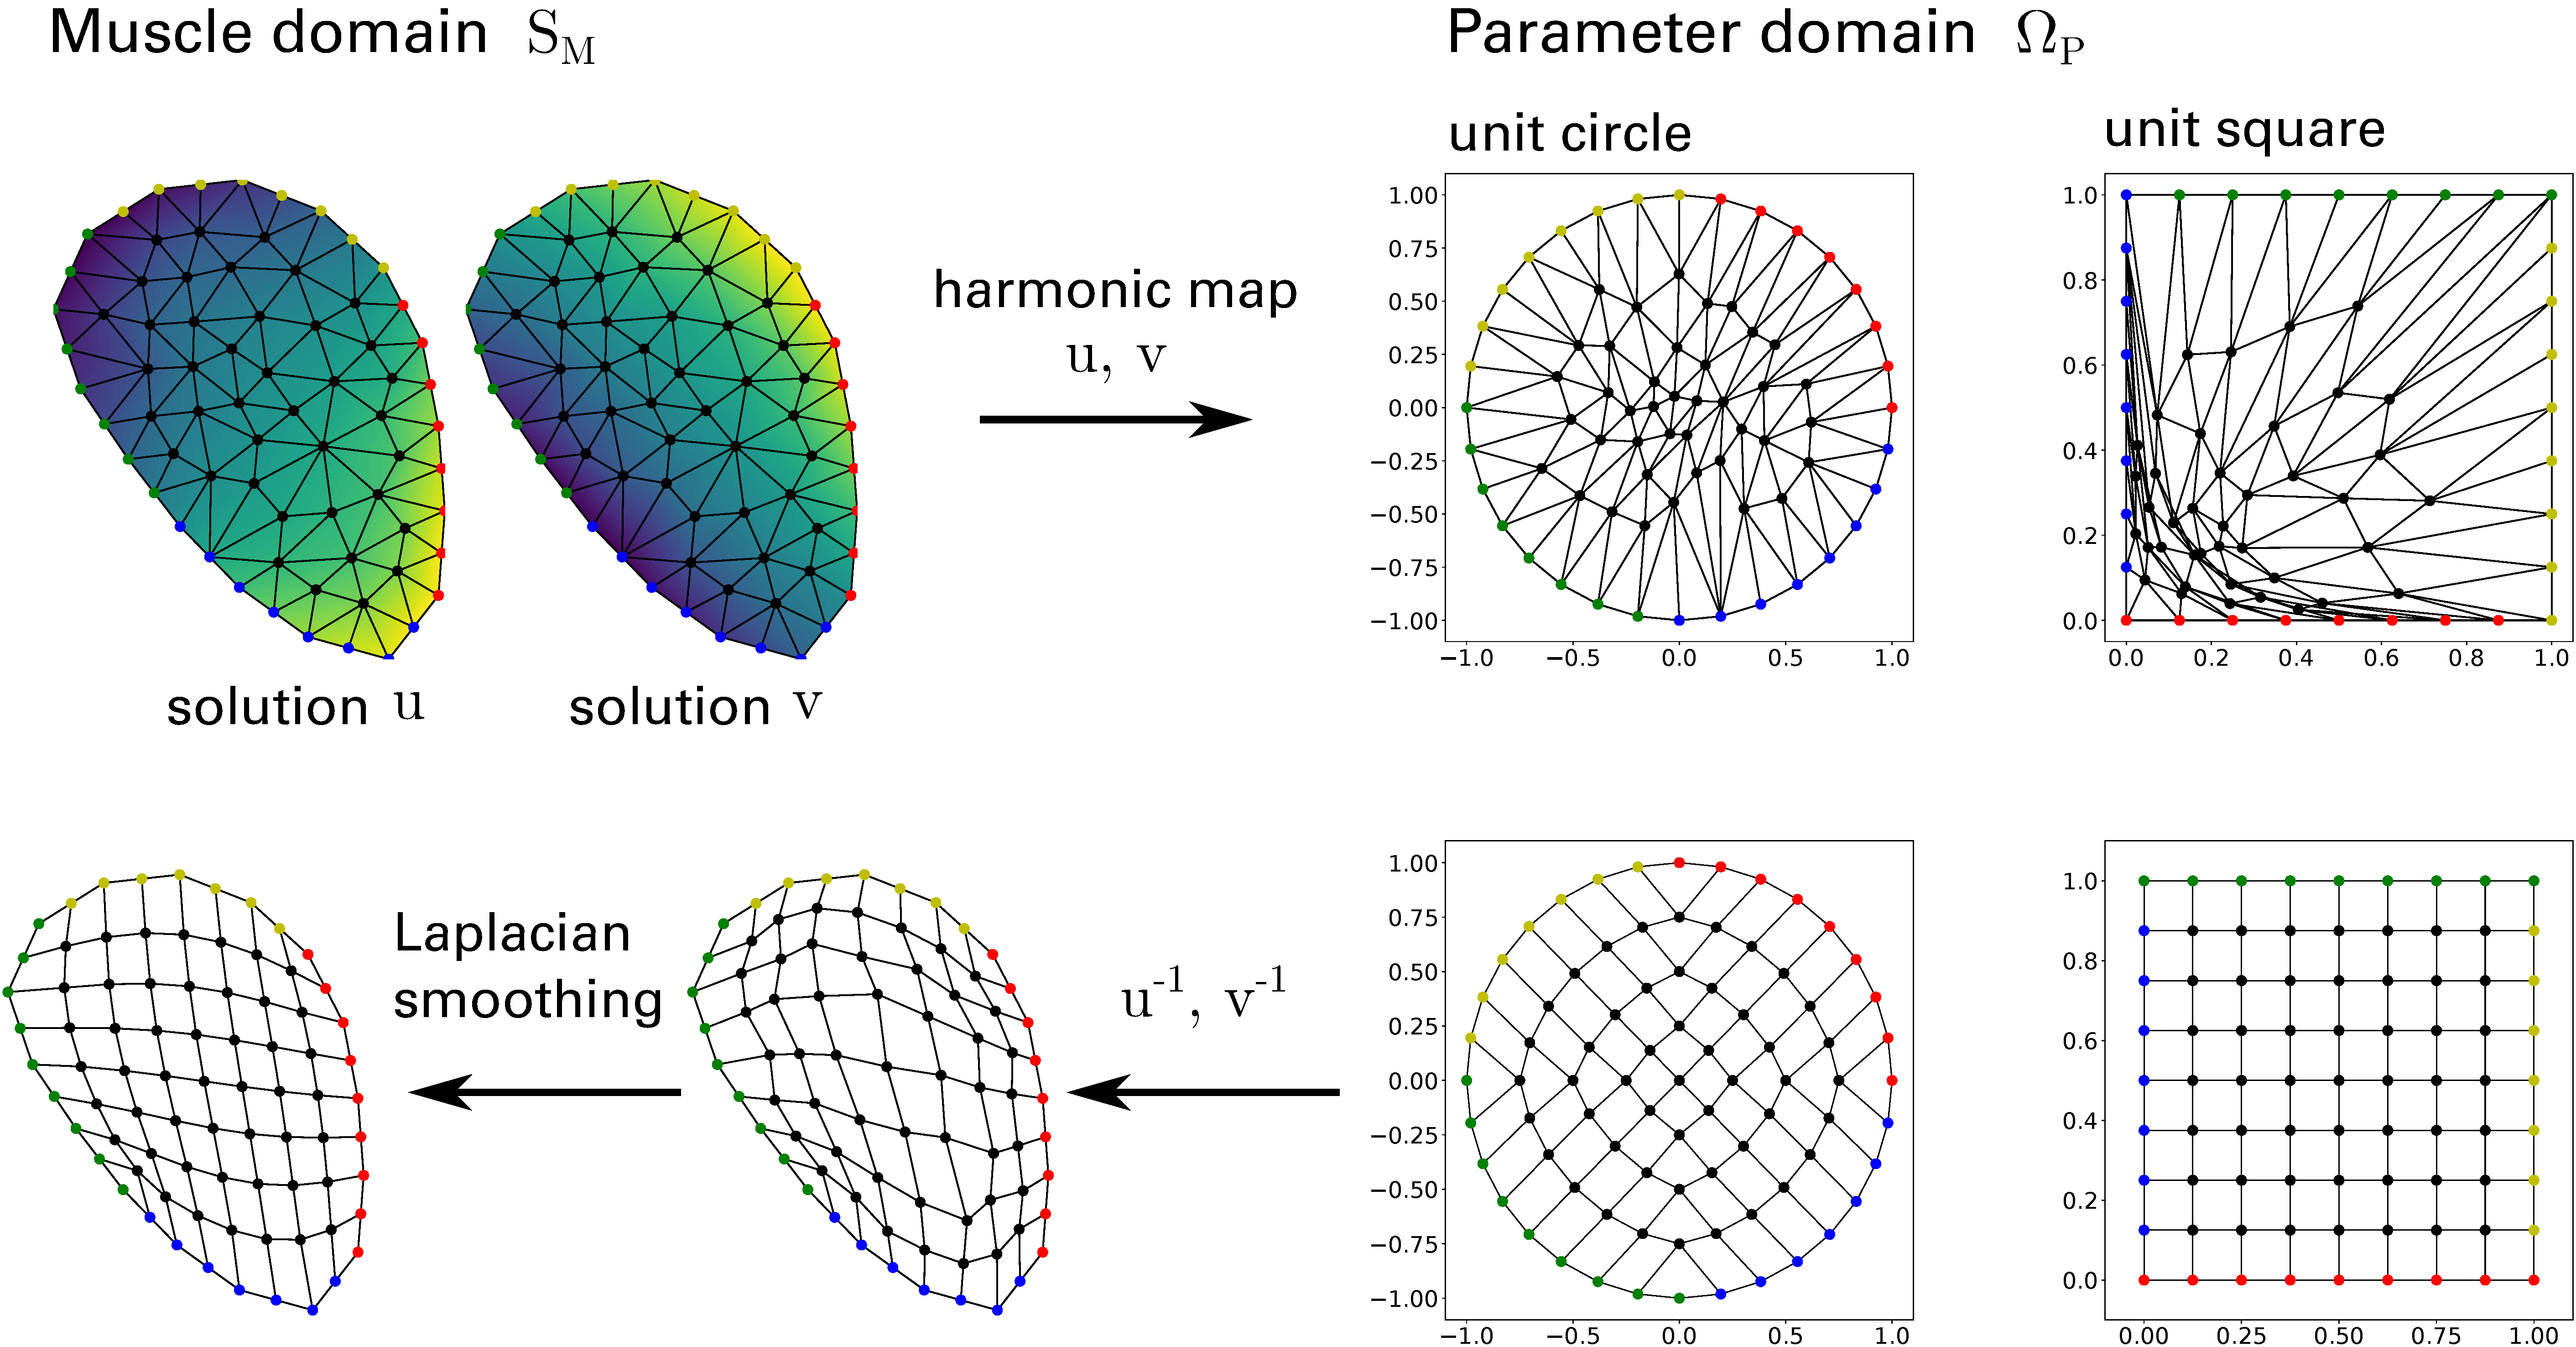
\includegraphics[width=\textwidth]{images/fiber_creation/harmonic_map_scheme_circle_square.pdf}%
  \caption{Generation of the muscle meshes, overview of the mapping method between the muscle domain (left) and the parameter domain (right) using harmonic maps.}%
  \label{fig:harmonic_map_solution}%
\end{figure}%

\subsection{Slicing of the Geometry}\label{sec:slicing_of_the_geometry}
The first step in line \ref{alg:1.1} of \cref{alg:serial_algorithm_1} slices the geometry. This means that horizontal \emph{slices} of the cross sectional area are extracted from the surface mesh. First, the muscle is divided into equidistant positions $z_i, i=1,\dots,n$ along the $z$-axis where the slices are to be extracted. As can be seen in \cref{fig:serial_alg_0}, $n=13$ $z$ coordinates are selected. Next, for every position $z_i$, all surface triangles $T_j$ that intersect the plane $Z_i = \{\bfp=(x,y,z) \mid z=z_i$\} are considered and the intersection lines $P = T_j \cap Z_i$ are computed. The method of computing plane-triangle intersection is described in the following.

Given is a triangle $T$ with points $\bfp^{1},\bfp^2,\bfp^3 ∈ \R^3$ and a value $\hat{z}$, the result is the set of points $P = T ∩ \{\bfp = (\bfp_x,\bfp_y,\bfp_z) \mid \bfp_z=\hat{z}\}$ which corresponds to a line segment $\overline{\bfp^a\bfp^b}$. 

We describe the points in the triangle by two barycentric coordinates $\xi_1$ and $\xi_2$ as
\begin{equation}\label{eq:barycentric_triangle}
  \begin{array}{lll}
    \bfp(ξ_1,ξ_2) = (1-ξ_1-ξ_2)\,\bfp^{1} + \xi_1\,\bfp^{2} + \xi_2\,\bfp^{3},  \\[4mm]
    \text{with }\xi_1+\xi_2 \leq 1, \quad 0 \leq \xi_1,\xi_2 \leq 1.
  \end{array}
\end{equation}
$\bfp_z(ξ_1,ξ_2) = \hat{z}$ defines the equation for the line through the points $\bfp^a$ and $\bfp^b$ in barycentric coordinates. The solution is given as
\begin{equation*}
  \begin{array}{lll}
    ξ_1 = m\cdot ξ_2 + c,\quad
    m = -\dfrac{\bfp_z^{3} - \bfp_z^{1}}{\bfp_z^{2} - \bfp_z^{1}}, \quad c = \dfrac{\hat{z} - \bfp_z^{1}}{\bfp_z^{2} - \bfp_z^{1}}, \quad \bfp_z^2 \neq \bfp_z^1.
  \end{array}
\end{equation*}
For $\bfp_z^1 = \bfp_z^2 \neq \bfp_z^3$ we swap $\bfp_z^2$ and $\bfp_z^3$.

%
%  # x(xi1,xi2) = (1-xi1-xi2)*x^{1} + xi1*x^{2} + xi2*x^{3},  xi1+xi2 <= 1, 0 <= xi1,xi2 <= 1
%  # x_3(xi1,xi2) = z_value  =>  (1-xi1-xi2)*x^{1} + xi1*x^{2} + xi2*x^{3} = z_value
%  #                         =>  xi1*(x^{2} - x^{1})  +  xi2*(x^{3} - x^{1})  =  z_value - x^{1}
%  #                         =>  xi2 = ((z_value - x^{1}) - xi1*(x^{2} - x^{1})) / (x^{3} - x^{1})
%  #                         =>  xi2 = (z_value - x^{1})/(x^{3} - x^{1}) - xi1 * (x^{2} - x^{1})/(x^{3} - x^{1})
%  #                         =>  xi1 = (z_value - x^{1}) / (x^{2} - x^{1})  - xi2 * (x^{3} - x^{1}) / (x^{2} - %x^{1}) 
Next, the end points of the line segment $\overline{\bfp^a\bfp^b}$ are determined.
We consider the three sides $\overline{\bfp^1\bfp^2}, \overline{\bfp^2\bfp^3}$ and $\overline{\bfp^3\bfp^1}$ of the triangle and check which of them are intersected by the $z=\hat{z}$ plane by the following three conditions:
\begin{enumerate}
\item On the triangle side $\overline{\bfp^1\bfp^2}$ the condition $ξ_2 = 0$ holds and the side intersects the plane 
at $\bfp(c,0)$ 
iff $0 \leq c \leq 1$. 
\item Similarly, on the triangle side $\overline{\bfp^1\bfp^3}$ we have the condition $ξ_1 = 0$ and the side intersects the plane 
at $\bfp(0,-c/m)$ 
iff $m\neq 0 \wedge 0 \leq -c/m \leq 1$. 
\item The third triangle side $\overline{\bfp^2\bfp^3}$ is intersected for $\hat{ξ}_1=(c+m) / (1+m)$
at $\bfp(\hat{ξ}_1,1-\hat{ξ}_1)$ 
iff ${m \neq -1 \wedge 0 \leq \hat{ξ}_1 \leq 1}$.
\end{enumerate}
If two of these three conditions for intersection of the triangle sides are met, there is an intersecting line segment $\overline{\bfp^a\bfp^b}$ with $\bfp^a \neq \bfp^b$ and the two intersection points $\bfp^a$ and $\bfp^b$ on the triangle sides are determined as stated above. The trival cases $\bfp^a = \bfp^b$ and the case where $\bfp^a$ and $\bfp^b$ are equal to two of the triangle corners $\bfp^1, \bfp^2$ and $\bfp^3$ are handled separately in our implementation.

After the presented computations are performed for all planes $Z_i$ and all triangles $T_j$, we have a number of line segments that form a geometric \say{ring} for each $z$ plane. The line segments are ordered according to their adjacency and a counter-clockwise orientation with respect to the $z$ axis is ensured.
The length of each ring is computed. A number $m=16$ of equidistant points is selected on each ring.

Because the selected points on the rings are later used as boundary points of the resulting 3D mesh, their position relative to each other on different rings should be in a tidy manner. The positioning should enable straight connection lines in longitudinal direction of the muscle connecting the points on every ring. For illustration, \cref{fig:serial_alg_0} shows such a configuration of properly positioned ring points. Connecting the points from top to bottom is possible with smooth lines rather than zig-zag lines. In result, the outer surface of the final mesh in \cref{fig:serial_alg_8} consists of a smooth quadrilateral mesh.

With given rings and number $m$ of equidistant points per ring, only the position of one point per ring is not yet fixed. To close the definition, in the following we formulate a first condition that relates the point positions of two neighboring rings and a second condition for one point at the bottom-most ring.

As mentioned, the first condition should ensure that the point positions on neighboring rings are as similar as possible. This is done by minimizing the distance between the first points on every ring.
In the algorithm, the $z$ planes are traversed from bottom to top. 
The first point $\tilde{\bfp}_{i,0}$ on a ring at $z=z_i$ is determined from the first point $\tilde{\bfp}_{i-1,0}$ of the previous ring at $z=z_{i-1}$ as the one with the minimal distance $|\tilde{\bfp}_{i,0} - \tilde{\bfp}_{i-1,0}|$. 
Thus, the searched point $\tilde{\bfp}_{i,0}$ has the property that the line between $\tilde{\bfp}_{i,0}$ and $\tilde{\bfp}_{i-1,0}$ and the tangent of the ring are perpendicular.

Given any point $\bfp$ on the ring at $z_i$ and the tangent vector $\bfu$ at this point, we can project the connection vector $\bfv$ from $\bfp$ to the start point $\tilde{\bfp}_{i-1,0}$ of the previous ring, $\bfv = \tilde{\bfp}_{i-1,0} - \bfp$, onto the tangent $\bfu$. This leads to the plumb foot point $\bfp_0$ by the computation
\begin{equation*}
  \begin{array}{lll}
    \bfp_0 = \bfp + t\,\bfu \quad \text{with }t = \dfrac{\bfv \cdot \bfu}{|\bfu|^2}.
  \end{array}
\end{equation*}
Performing this calculation for every line segment $u$ on a ring allows to select the plumb foot $\bfp_0$ with the smallest distance to the start point $\tilde{\bfp}_{i-1,0}$ of the previous ring to be the start point $\tilde{\bfp}_{i,0}$ of the current ring. This is the point that fulfills the first condition.

With this first condition, all points are only fixed relative to each other. The definition of one point, the start point $\tilde{\bfp}_{0,0}$ of the bottom-most ring, is missing. The second condition fixes this point by a prescribed plane at $x = \hat{x}$ and selects $\tilde{\bfp}_{0,0}$ such that its $x$ coordinate lies in this plane. From the (usually two) points that meet this condition, the one with lower $y$ coordinate is selected. The actual value of $\hat{x}$ is determined experimentally such that the resulting point positions are visually uniform. Not every value leads to a good result because of the shape of the biceps muscle, especially the groove where the humerus bone is located.

The resulting grid of points on the biceps surface is visualized in \cref{fig:serial_alg_0}. It can be seen that all points of the same ring have the same $z$ coordinate. By connecting neighboring points horizontally and vertically, a regular grid can be formed. This overall grid in this $x$-$z$ perspective view looks relatively uniform, e.g., compared with the gray surface triangulation mesh of the biceps geometry. The spacing between the points is lower at the top and bottom of the muscle because of the smaller circumference at these locations.

%
\begin{figure}%
  \centering%
  \begin{subfigure}[t]{0.45\textwidth}%
    \centering%
    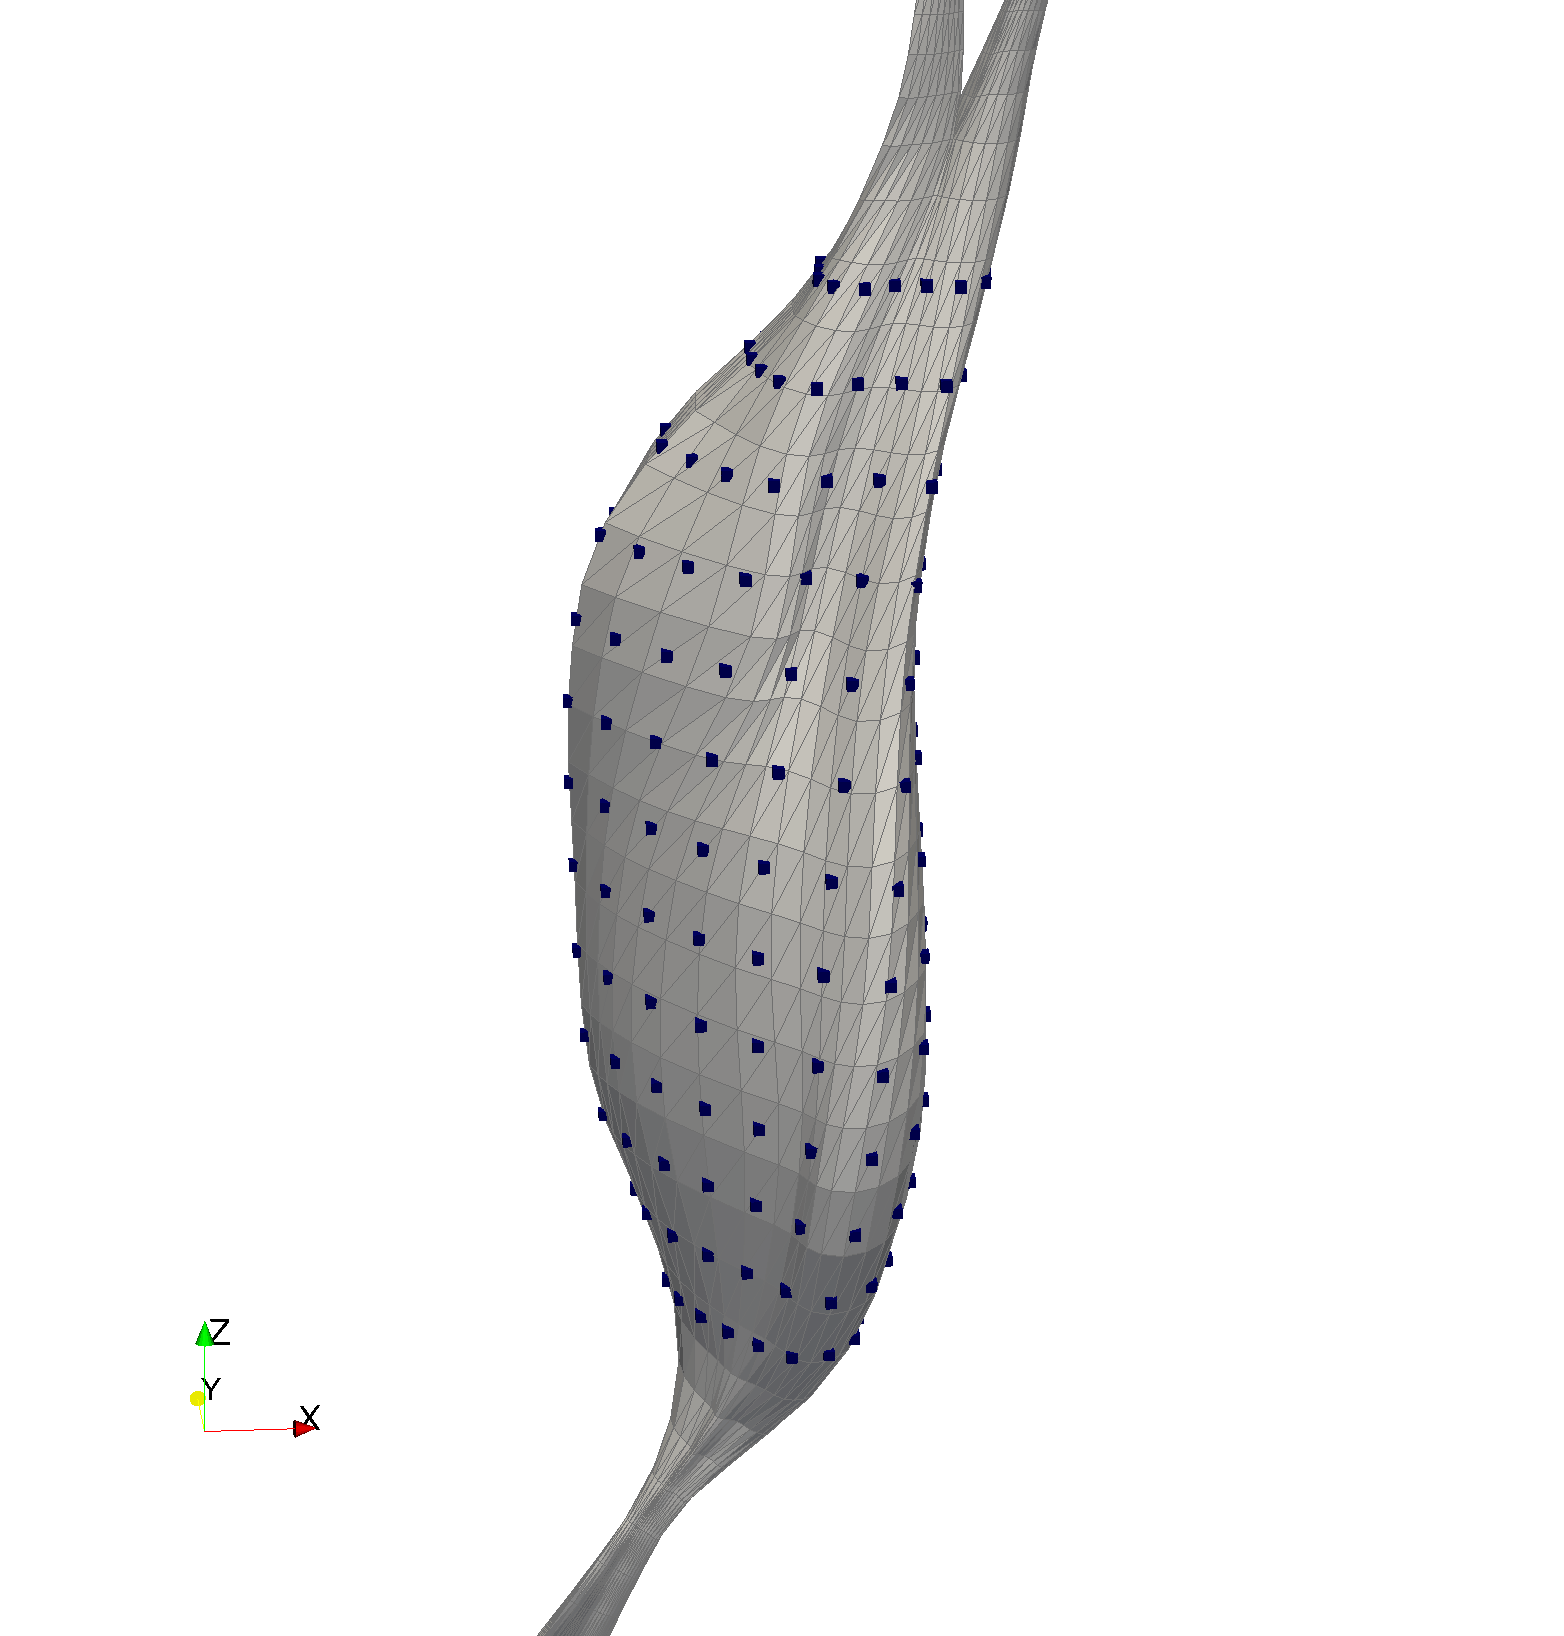
\includegraphics[height=9cm]{images/fiber_creation/serial_alg_0.png}% [trim=left bottom right top, clip]
    \caption{Extracted boundary points (blue) on the biceps surface mesh (gray). This is the result of line \ref{alg:1.1} in \cref{alg:serial_algorithm_1}.}%
    \label{fig:serial_alg_0}%
  \end{subfigure}
  \quad
  \begin{subfigure}[t]{0.51\textwidth}%
    \centering%
    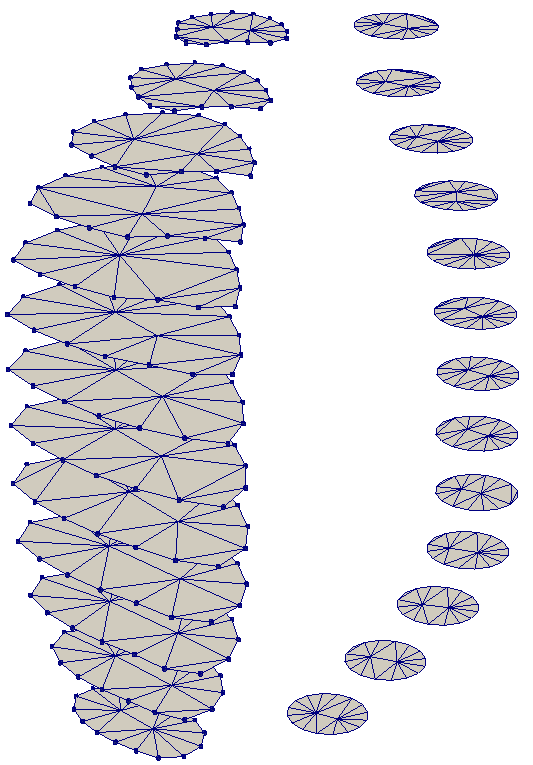
\includegraphics[height=9cm]{images/fiber_creation/serial_alg_3.png}%
    \caption{The generated triangulation of the slices (left) and the image $\bfy(\bfx)$ of the triangulation under the harmonic map (right). This figure shows the result of lines \ref{alg:1.2} and \ref{alg:1.3} in \cref{alg:serial_algorithm_1}.}%
    \label{fig:serial_alg_3}%
  \end{subfigure}\\
  \centering%
  \begin{subfigure}[t]{0.49\textwidth}%
    \centering%
    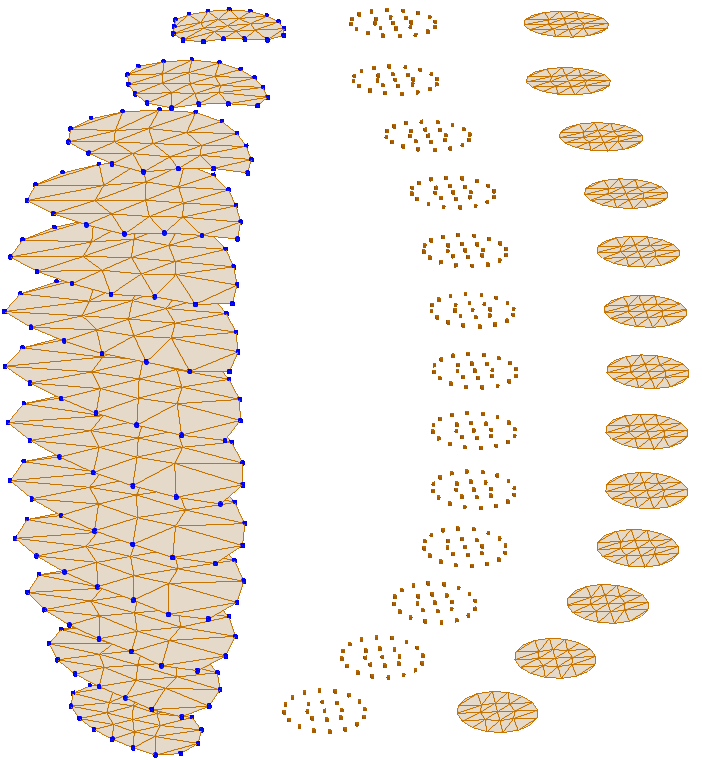
\includegraphics[height=9cm]{images/fiber_creation/serial_alg_4_orange.png}%
    \caption{Grid in parameter space (right) and muscle domain (left), result after line \ref{alg:1.4} in \cref{alg:serial_algorithm_1}.}%
    \label{fig:serial_alg_4}%
  \end{subfigure}
  \hfill{}
  \begin{subfigure}[t]{0.4\textwidth}%
    \centering%
    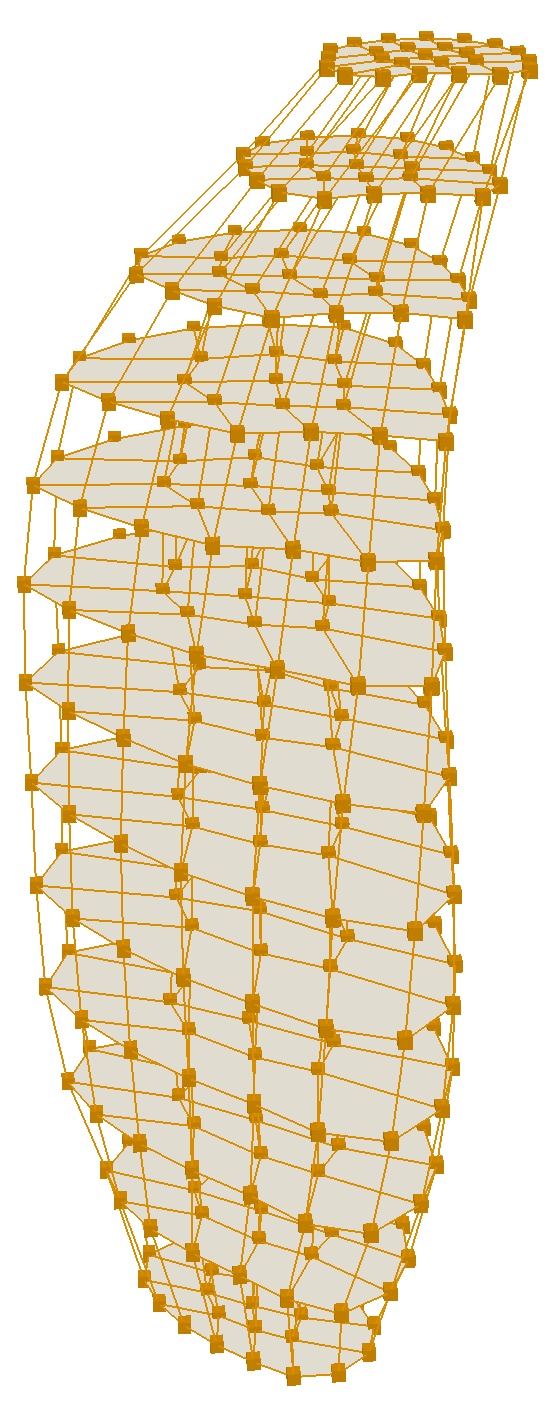
\includegraphics[height=9cm]{images/fiber_creation/serial_alg_8_orange.png}%
    \caption{3D elements formed by connecting the slices in line \ref{alg:1.5} in \cref{alg:serial_algorithm_1}.}%
    \label{fig:serial_alg_8}%
  \end{subfigure}
  \caption{Steps of the serial algorithm for 3D mesh generation, \cref{alg:serial_algorithm_1}, executed directly on the surface mesh of the biceps muscle (not the B-spline surface).}%
  \label{fig:serial_alg}%
\end{figure}%
%

\subsection{Triangulation of the Slices}\label{sec:triangulation_of_the_slices}
The points of each ring enclose a planar, polygonal surface, a \emph{slice} $S_M$ of the muscle.
The next step in the algorithm, line \ref{alg:1.2}, is to triangulate the extracted slices, i.e., to construct triangles that decompose the polygons. The result of this step is visualized on the left side in \cref{fig:serial_alg_3}.

We select three different methods to construct this triangulation. The first and second methods are based on Delaunay triangulations. The third method creates a custom triangulation using a simple construction scheme with only one additional point.
\Cref{fig:triangulations} visualizes results of the three methods for one slice.

The first method uses the tessellation algorithm from the spatial algorithms and data structures module of the Python package \emph{SciPy}. 
The Quickhull algorithm \cite{quickhull} is used which triangulates the convex hull of the points. In consequence, the triangulations of concave slices have triangles that lie outside the interior of the slice, which is a disadvantage. An advantage is that the triangulation uses all given points and no new points are added. However, this often results in meshes of lower quality than if adding additional points were allowed.
The example in \cref{fig:triangulation_0} shows such a concave slice. At the bottom of the domain, the triangles are outside the slice and almost degenerate.

The second method uses a Delaunay refinement algorithm described in \cite{Delaunay2002} and implementated in the \emph{Triangle} software \cite{shewchuk96b}. A conforming, constrained Delaunay triangulation is created. The triangulation correctly handles convex and concave domains.
Conforming means that the triangulation uses the given points at the boundary. Additional points on the boundary as well as in the interior are added. The triangulation is constraint to generate triangles with minimum angles of 20 degrees and a maximum area $A$ that is set to a value depending on the area of the bounding box. In consequence, the generated triangulations of all slices have a guaranteed mesh quality in terms of angles and about the same size and number of triangles.

Comparing the result of the second method in \cref{fig:triangulation_1} with the result of the first method in \cref{fig:triangulation_0} shows the better triangulation quality as the triangles all have larger angles.

The third method places one additional point at the center of gravity of the given points. Triangles are constructed by connecting the center point with two adjacent points on the boundary, for all given points. The resulting triangulation resembles a pie chart. For some extreme concave slices, this method also creates triangles that partly lie outside the slice, but this occurs rarely with muscle cross sections. The advantage of this approach is its simplicity.
\Cref{fig:triangulation_2} shows the result for an exemplary slice. In contrast to the first method, the third method creates a valid triangulation despite the concave domain.

\begin{figure}%
  \centering%
  \begin{subfigure}[t]{0.31\textwidth}%
    \centering%
    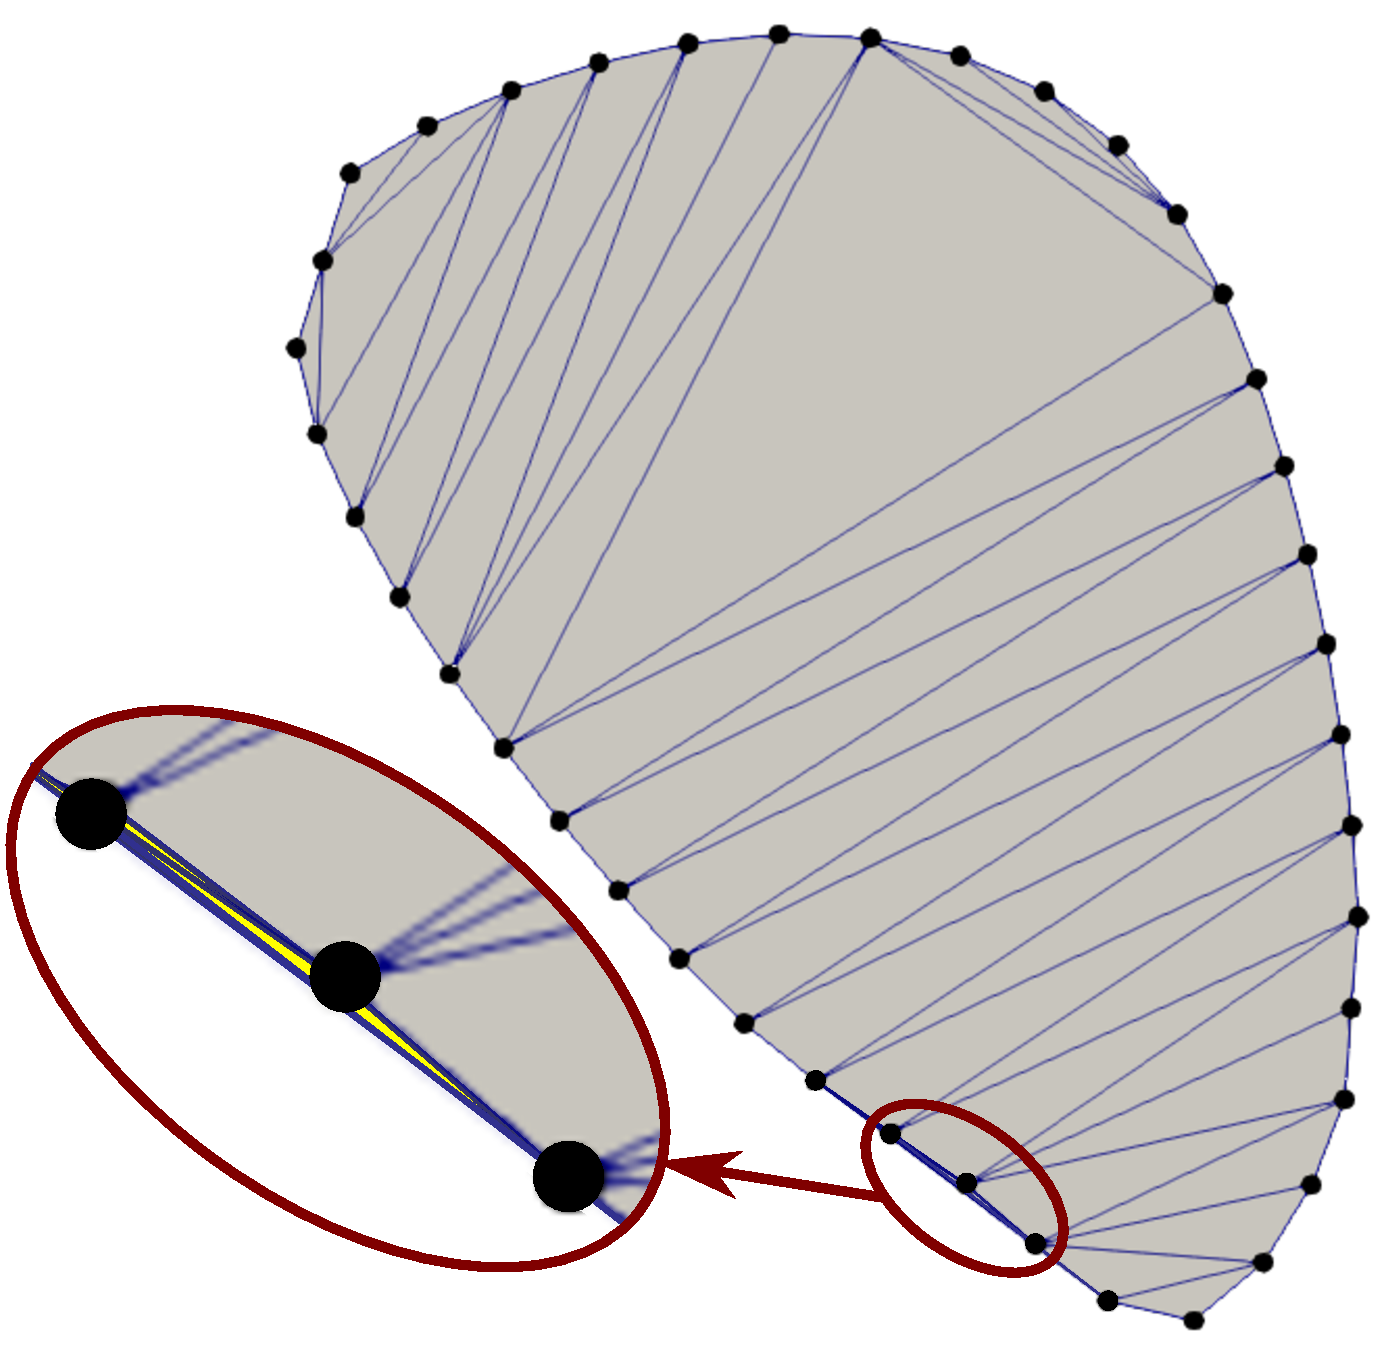
\includegraphics[height=55mm]{images/fiber_creation/triangulation_0.pdf}%
    \caption{First triangulation method}%
    \label{fig:triangulation_0}%
  \end{subfigure}
  \qquad
  \begin{subfigure}[t]{0.27\textwidth}%
    \centering%
    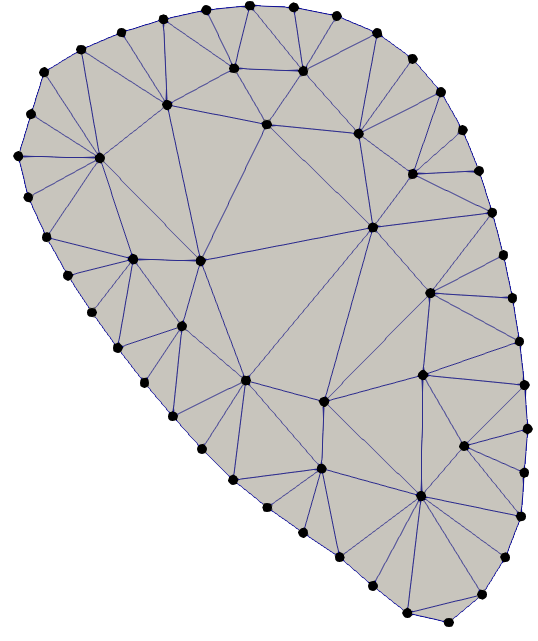
\includegraphics[height=55mm]{images/fiber_creation/triangulation_1.png}%
    \caption{Second trian\-gulation method}%
    \label{fig:triangulation_1}%
  \end{subfigure}
  \quad
  \begin{subfigure}[t]{0.32\textwidth}%
    \centering%
    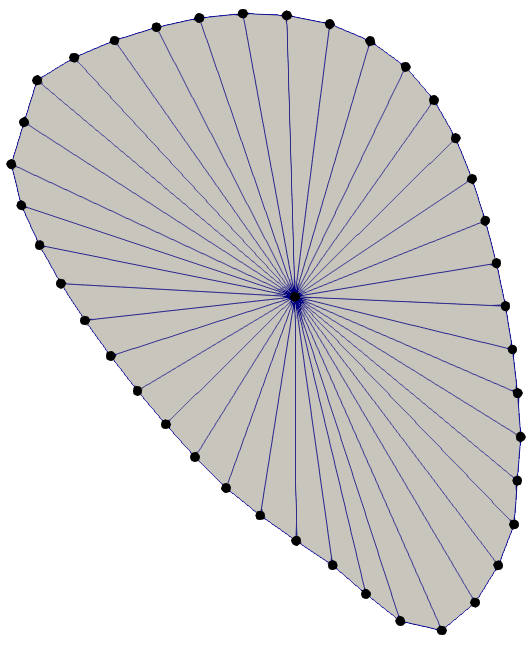
\includegraphics[height=55mm]{images/fiber_creation/triangulation_2.png}%
    \caption{Third triangulation method}%
    \label{fig:triangulation_2}%
  \end{subfigure}
  \caption{Intermediate step of 3D mesh generation: triangulation of slices, result of different triangulation methods for a slice in the center of the biceps muscle.}%
  \label{fig:triangulations}%
\end{figure}%

\subsection{Harmonic Maps}

Next, harmonic maps are created that allow to smoothly map a given 2D reference mesh onto an actual cross section of the muscle. The initial application of harmonic maps to meshes used for biomedical simulations is given by \cite{marchandise2010quality} and \cite{Marchandise2_2011}. The authors improve a given, oversampled surface mesh obtained from classical segmentation. This is done by partitioning the surface into multiple mesh partitions of zero genus (i.e., containing no holes) and transforming them to a reference space using harmonic maps. There, controlled remeshing is carried out before the transformation is reversed.

In our algorithm, harmonic maps are also used for the purpose of generating high quality meshes. In contrast to the literature, the mapping is based on the muscle slices instead of the surface. Also, different parameter domains are investigated.

A function $u: \Omega \to \R$ on a domain $\Omega \in \R^d$ is \emph{harmonic} if it is a solution of the Laplace equation $Δu = 0$.
From variational calculus, it is known that harmonic functions are extremals of the \emph{Dirichlet energy functional} \cite{weyl1940},
\begin{align*}
  E[u] = \dfrac12 \int_\Omega |\nabla u|^2 \,\d\bfx.
\end{align*}
For an intuitive understanding, the map $u$ can be seen as deforming an elastic material that is initially located tension-free in the domain $\Omega$.
Then, the Dirichlet energy $E[u]$ describes the total amount of squared stretch or elastic energy resulting from the tension that occurs in the deformed state. A harmonic map minimizes this total tension. Qualitatively, the map deforms neighborhoods of all points in $\Omega$ by a similar amount, thus, preserving geometrical structures in $\Omega$, e.g., given by a mesh. The idea of our approach is that 
applying a harmonic map on a mesh with good quality preserves the mesh quality also in the image under the map.

In \cref{alg:serial_algorithm_1}, computing the harmonic maps $u$ and $v$ is done in line \ref{alg:1.3}. For a given slice $S_M$, the functions $u$ and $v$ map from points $\bfx \in S_M$ to coordinates $u(\bfx),v(\bfx)\in \R$ of a parameter domain $\Omega_P \subset \R^2$. The parameter domain is either a unit circle or a unit square.

The vector $\bfy(\bfx) := (u(\bfx), v(\bfx))^\top$ for $\bfx \in S_M$ is interpreted as position in $\Omega_P$. The maps are constructed such that the boundary $∂S_M$ of the slice $S_M$ is mapped to the boundary $∂\Omega_P$ of the parameter domain $\Omega_P$ while preserving the distance between points on the boundary.
The mapping $\bfy: S_M \to \Omega_P$ is bijective and harmonic, i.e., the Laplacians of $u$ and $v$ are zero.
More specifically, $u : S_M \to \R$ and $v : S_M \to \R$ are solutions of
%
\begin{equation}\label{eq:def_harmonic_maps}
  \begin{array}{l}
    Δu(\bfx) = 0, \quad Δv(\bfx) = 0 \quad \forall \bfx \in S_M.
  \end{array}
\end{equation}
%
To derive suitable Dirichlet boundary conditions for these equations, we consider a uniform parametrization $\bfp:[0,1] \to ∂S_M$ of the boundary $∂S_M$ of the slice, i.e., 
%
\begin{align*}
  \p{l(t)}{t} = c \in \R \quad \forall t \in [0,1], \quad \text{where } l(t) := \i{0}{t} |\bfp'(\tau)| \,\d\tau.
\end{align*}
%
We require the image of the boundary parametrization in $\Omega_P$ to be also uniform, i.e.,%
\begin{align*}
  \p{l_P(t)}{t} = c_P \in \R \quad \forall t \in [0,1], \quad \text{where } l_P(t) := \i{0}{t} |\bfy'\big(\bfp(\tau\big)| \,\d\tau.
\end{align*}
%
Corresponding boundary points $\bfx_\text{M,boundary} \in S_M$ and $\bfx_\text{P,boundary} = (u_\text{P,boundary},v_\text{P,boundary})^\top$ can be defined. This leads to the following Dirichlet boundary conditions that close the definition in \cref{eq:def_harmonic_maps}:%
\begin{align}\label{eq:bc_harmonic_maps}
  u(\bfx_\text{M,boundary}) = u_\text{P,boundary}, \quad v(\bfx_\text{M,boundary}) = v_\text{P,boundary}.
\end{align}
%

Equations \eqref{eq:def_harmonic_maps} and \eqref{eq:bc_harmonic_maps} describe a boundary value problem of ordinary differential equations for $u$ and $v$. We solve it using the finite element method and the spatial discretization given by the triangulation of the slices.
Depending on the method of triangulation, a different number of degrees of freedom is given. For the first method with the Quickhull algorithm, no degree of freedom is present and no system of equations needs to be solved. Then, the mapping is only a FE interpolation of the boundary mapping.
For the third method, only one degree of freedom for the center point needs to be computed. The second method has as many degrees of freedom as there are additional points inserted during the Delaunay refinement.

The first step is to compute the prescribed boundary points $\bfx_\text{P,boundary}$ in parameter space. When using the first and third triangulation methods, the boundary points on the slices are  equidistant and therefore the same number of points need to be sampled equidistantly on the boundary $∂\Omega_P$ of the parameter space.
If the second triangulation method, which potentially adds additional points is used, the same number of points  are created on the boundary $∂\Omega_P$ of the slice as are given on the slice $∂S_M$. The boundary points are created such that the relations of their distances are the same on $∂\Omega_P$ as for the original points on $∂S_M$.

Using the standard procedure of the finite element method for $Δu(\bfx) = 0$ on $S_M$ and $u=f(\bfx)$ on $∂S_M$, e.g., as outlined in \cite{Remacle2010}, leads to the weak form with ansatz and test functions $\phi$,
\begin{align}\label{eq:est_fe_w}
    \i{S_M}{} (\nabla u^\top \nabla \phi + \nabla f(\bfx)^\top \nabla \phi) \,\d \bfx = 0 \quad \forall \phi \in \mathcal{H}_0^1.
\end{align}
Standard linear hat functions are used on the triangles, such that they provide the interpolation property $\phi_i(\bfx_j) = \delta_{ij}$. Using the barycentric parametrization of triangles with points $\bfp^1,\bfp^2$ and $\bfp^3$ introduced in \cref{eq:barycentric_triangle}, we define the ansatz functions and get their derivatives within the elements by:
%
\begin{align*}
  \phi^{(e)}_1 &= (1 - \xi_1)(1 - \xi_2), \quad&
  \phi^{(e)}_2 &= \xi_1 (1 - \xi_2), \quad &
  \phi^{(e)}_3 &= (1 - \xi_1) \xi_2,\\[4mm]
  \nabla \phi^{(e)}_1 &= (\xi_2-1, \xi_1 - 1)^\top, \quad&
  \nabla \phi^{(e)}_2 &= (1-\xi_2, -\xi_1)^\top, \quad&
  \nabla \phi^{(e)}_3 &= (-\xi_2, 1-\xi_1)^\top.
\end{align*}
The superscript $\square^{(e)}$ refers to the definition of the functions within elements. The global assembly involves composing the global nodal functions $\phi_i(\bfx)$ for nodes indexed by $i=1, \dots, n_\text{nodes}$ and using a mapping between the barycentric coordinates $\xi_1,\xi_2 \in [0,1]^2$ inside the elements to the global coordinates $\bfx \in S_M$.
Inserting the discretization
\begin{align*}
  u_h(\bfx) = \s{i=1}{n_\text{nodes}} u_i\,\phi_i(\xi_1(\bfx), \xi_2(\bfx))
\end{align*}
into \cref{eq:est_fe_w} leads to the form
\begin{equation}\label{eq:est_weak_form}
  \begin{array}{lll}
    \s{i=1}{n_\text{nodes}}u_i \i{S_M}{} \nabla_\bfx \phi_i^\top \nabla_\bfx \phi_j \,\d\bfx + \s{i=1}{n_\text{nodes}} f_i \i{S_M}{} \nabla_\bfx \phi_i^\top \nabla_\bfx \phi_j \,\d \bfx = 0\,\quad \forall j=1,\dots,n_\text{nodes}.
  \end{array}
\end{equation}
The integrations are executed element-wise and over the elemental coordinates $\xi_1,\xi_2$. 
The transformation to elemental coordinates involves the computation of the Jacobian $J=\d\bfx/\d\bfxi$ of the mapping between element coordinates $\bfxi = (ξ_1,ξ_2)$ and global coordinates $\bfx$. From the definition in \cref{eq:barycentric_triangle}, it follows that
\begin{align*}
  J = \d{\bfx}{\bfxi} = [\bfp^2-\bfp^1, \bfp^3-\bfp^1].\\[4mm]
\end{align*}
The metric tensor for this mapping is given by
\begin{align*}
  \mathcal{M} := \left(\d{x}{\bfxi}\right)^T \left(\d{x}{\bfxi}\right).
\end{align*}
%
The transformation of the integrals in \cref{eq:est_weak_form} introduces an additional integration factor $\sqrt{\det{\mathcal{M}}}$.
We get the following matrix equation:
\begin{align}\label{eq:est_fe_system}
  M_u \bfu = -M_f\,\bff,
\end{align}
with the vector $\bfu$ of nodal solution values, the vector $\bff$ of nodal Dirichlet boundary condition values at the boundary and the global stiffness matrices $M_u$ and $M_f$. The two global stiffness matrices are assembled from the element stiffness matrices $M^\text{(e)}$ for the degrees of freedom at all nodes respectively at the boundary nodes. The entries of the element stiffness matrices are given by
\begin{align*}
  M^\text{(e)}_{i,j} = \i{0}{1}\i{0}{1-\xi_1}   \nabla \phi_i^{(e)}(\xi_1,\xi_2)^\top \, \mathcal{M}^{-1} \, \nabla \phi_j^{(e)}(\xi_1,\xi_2) \, \sqrt{\det{\mathcal{M}}}  \,\d\xi_2\d\xi_1.
\end{align*}

By solving \cref{eq:est_fe_system} for $\bfu$, we get the discretized harmonic map $u$.
The finite element formulation and computation for $v$ is analog and uses the same global stiffness matrices.

\Cref{fig:harmonic_map_solution0} visualizes the triangulation of $S_M$ and the solutions $u(\bfx)$ and $v(\bfx)$ for a circular parameter domain $\Omega_P$ and an exemplary muscle slice in the first two plots. The color range from bright yellow to dark violet corresponds to increasing values of $u$ and $v$. It can be seen that the $u$ values increase from left to right whereas the $v$ values increase from bottom to top, corresponding to the horizontal and vertical coordinate axes $y_1$ and $y_2$ of $\Omega_P$.


Applying the computed harmonic map $\bfy(\bfx)$ to the triangulation of the slices results in a triangulation of the parameter domain $\Omega_P$. This is shown in the third plot of \cref{fig:harmonic_map_solution0} and in \cref{fig:serial_alg_3}.
In both figures, the triangulation of the slices was generated using the second triangulation method with the constrained Delaunay triangulation. On the right side of \cref{fig:serial_alg_3}, the image $\bfy(\bfx)$ under the harmonic map of the triangulation in the slices is shown on the unit circle parameter domain.

\begin{figure}%
  \centering%
  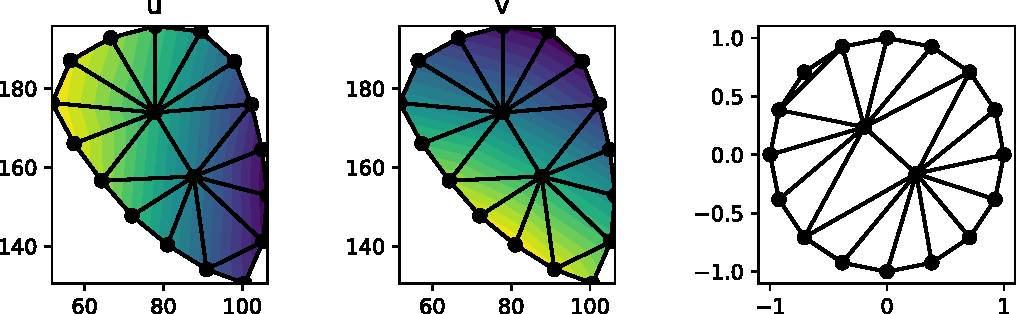
\includegraphics[width=\textwidth]{images/fiber_creation/harmonic_map_9b.pdf}%
  \caption{Quality improvement of muscle slice meshes as a basis for 3D mesh generation: Initial triangulations and harmonic map for a slice $S_M$ of the biceps muscle. The first two plots show the solutions of $u$ and $v$ on the slice $S_M$. The third plot shows the image in $\Omega_P$ of the triangulation in $S_M$ under the harmonic map.}%
  \label{fig:harmonic_map_solution0}%
\end{figure}%

\subsection{Construction of a Regular Grid in the Parameter Domain}
The next step in \cref{alg:serial_algorithm_1} is the construction of a 2D structured, regular grid in the parameter domain $\Omega_P$, as stated in line \ref{alg:1.4}. This grid will then be mapped to the slices $S_M$. Creating a structured grid of quadrilateral elements in a given domain is also called \emph{quadrangulation}.

The parameter domain $\Omega_P$ can be selected to be either a unit square or a unit circle. For both choices, two different schemes how to generate a grid with a given number of cells can be selected.
\Cref{fig:quads} shows all four possiblities.

The first scheme, \cref{fig:quad_1}, uses an equidistant regular grid in a unit square. This is the easiest possibility to generate a quadrangulated reference domain. A possible issue is induced by the corners of the square. The grid will be mapped to a cross section of the muscle which has no sharp corners. Therefore, the cells of the grid will be distorted at the images of the corners, usually shortening diagonals that point towards the corners and lengthening the other diagonals. This assumption motivates the second scheme in \cref{fig:quad_2}. Here, the elements are already distorted in the described manner, with increasing distortion closer to the corners. The rationale is that the mapped cells in $S_M$ will then be less distorted.

We construct our second quadrangulation scheme of the unit square as follows. The diagonals of the square divide the domain into bottom, top, left and right quarters, which are considered separately.
For example, the bottom quarter is the triangle that is formed by the corner points $(0,0), (1,0)$ and the center point $(\frac12,\frac12)$ of the square. In the bottom quarter, the horizontal $x$ coordinate of a point $(x,y)$ in a uniform grid can be described by $x = \frac12 + \textrm{tan}(\phi)\,(\frac12-y)$ where $\phi$ is the angle between a line through $(x,y)$ and the center point $(\frac12,\frac12)$ and the $y$-axis. The points of the adjusted grid in the quadrangulation scheme are constructed by altering the value of $\phi$.
On every horizontal series of points in the bottom quarter, $\phi$ is varied linearly in $[-\pi/4,\pi/4]$ instead of the nonlinear progression according to the actual angle. This leads to the larger spacing between points near the diagonals. All four quarters are treated analogously to produce the shown symmetric pattern.

A different approach is to use a unit circle, which has no corners and therefore might resemble a muscle cross section more consistently. The first scheme of the unit circle is given in \cref{fig:quad_0}. It uses the radial and circumferential directions for the two dimensions of the grid. A disadvantage of this scheme is that the quadrilaterals at the center are degenerated to triangles. Additionally, the area of the cells varies significantly and the outer cells have unequal side lengths. 

To remedy this problem, we develop the second scheme given in \cref{fig:quad_3}. When traversing from the outer boundary towards the center point and considering the circumferential lines of grid points, the circle morphs into a square as the number of grid points decreases. This approach has the disadvantage that some cells have an inner angle of nearly \SI{180}{\degree}, especially four elements at the boundary. Apart from that, all elements have similar sized sides and angles.
The construction of this scheme is similar to the approach of scheme 2 on the unit square in that the domain is also divided into four quarters. However, different formulas for the point coordinates $(x,y)$ depending on the angle $\phi$ are used.
The detailed construction formulas of all four presented quadrangulation schemes are provided by their implementation in the code. The script \code{plot_quadrangulation_schemes.py} constructs and visualizes the four schemes with a configurable number of grid points.


Each construction scheme allows to specify the (squared) number of nodes and in consequence the number of cells. The examples in \cref{fig:quad_1,fig:quad_2,fig:quad_3} have $11 \times 11$ nodes and $10 \times 10$ cells. For \cref{fig:quad_0}, the numbers are slightly different. There are $10 \times (11 + 1)$ nodes resulting in $10 \times 11$ cells.

\begin{figure}%
  \centering%
  \begin{subfigure}[t]{0.48\textwidth}%
    \centering%
    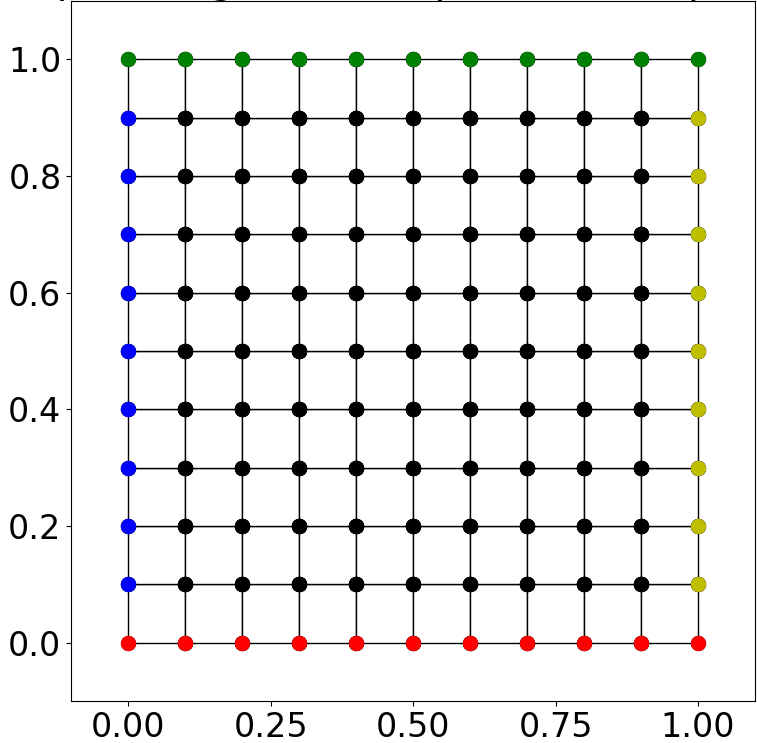
\includegraphics[width=\textwidth]{images/fiber_creation/quad_1.png}%
    \caption{Unit square, scheme 1}%
    \label{fig:quad_1}%
  \end{subfigure}
  \quad
  \begin{subfigure}[t]{0.48\textwidth}%
    \centering%
    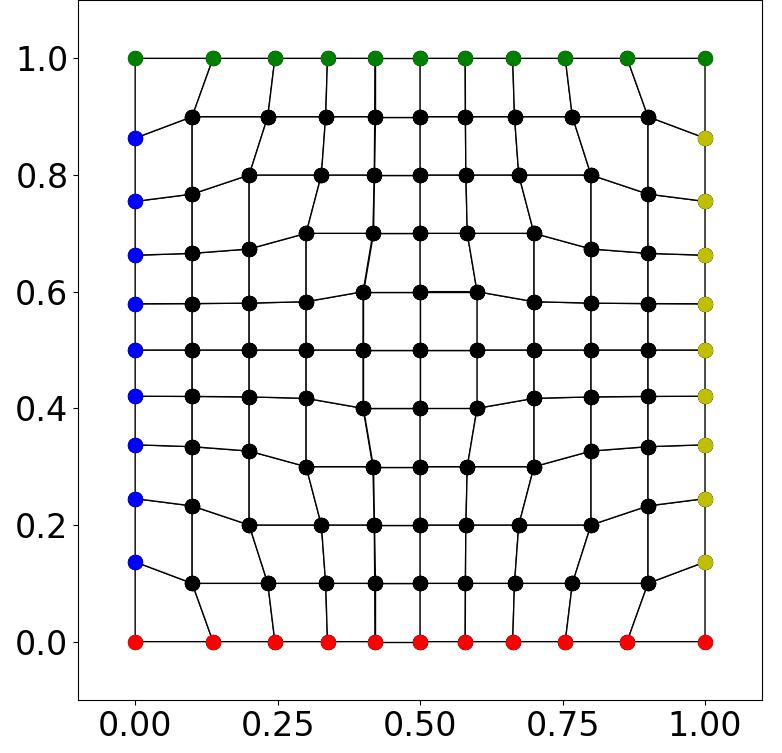
\includegraphics[width=\textwidth]{images/fiber_creation/quad_2.png}%
    \caption{Unit square, scheme 2}%
    \label{fig:quad_2}%
  \end{subfigure}
  \begin{subfigure}[t]{0.48\textwidth}%
    \centering%
    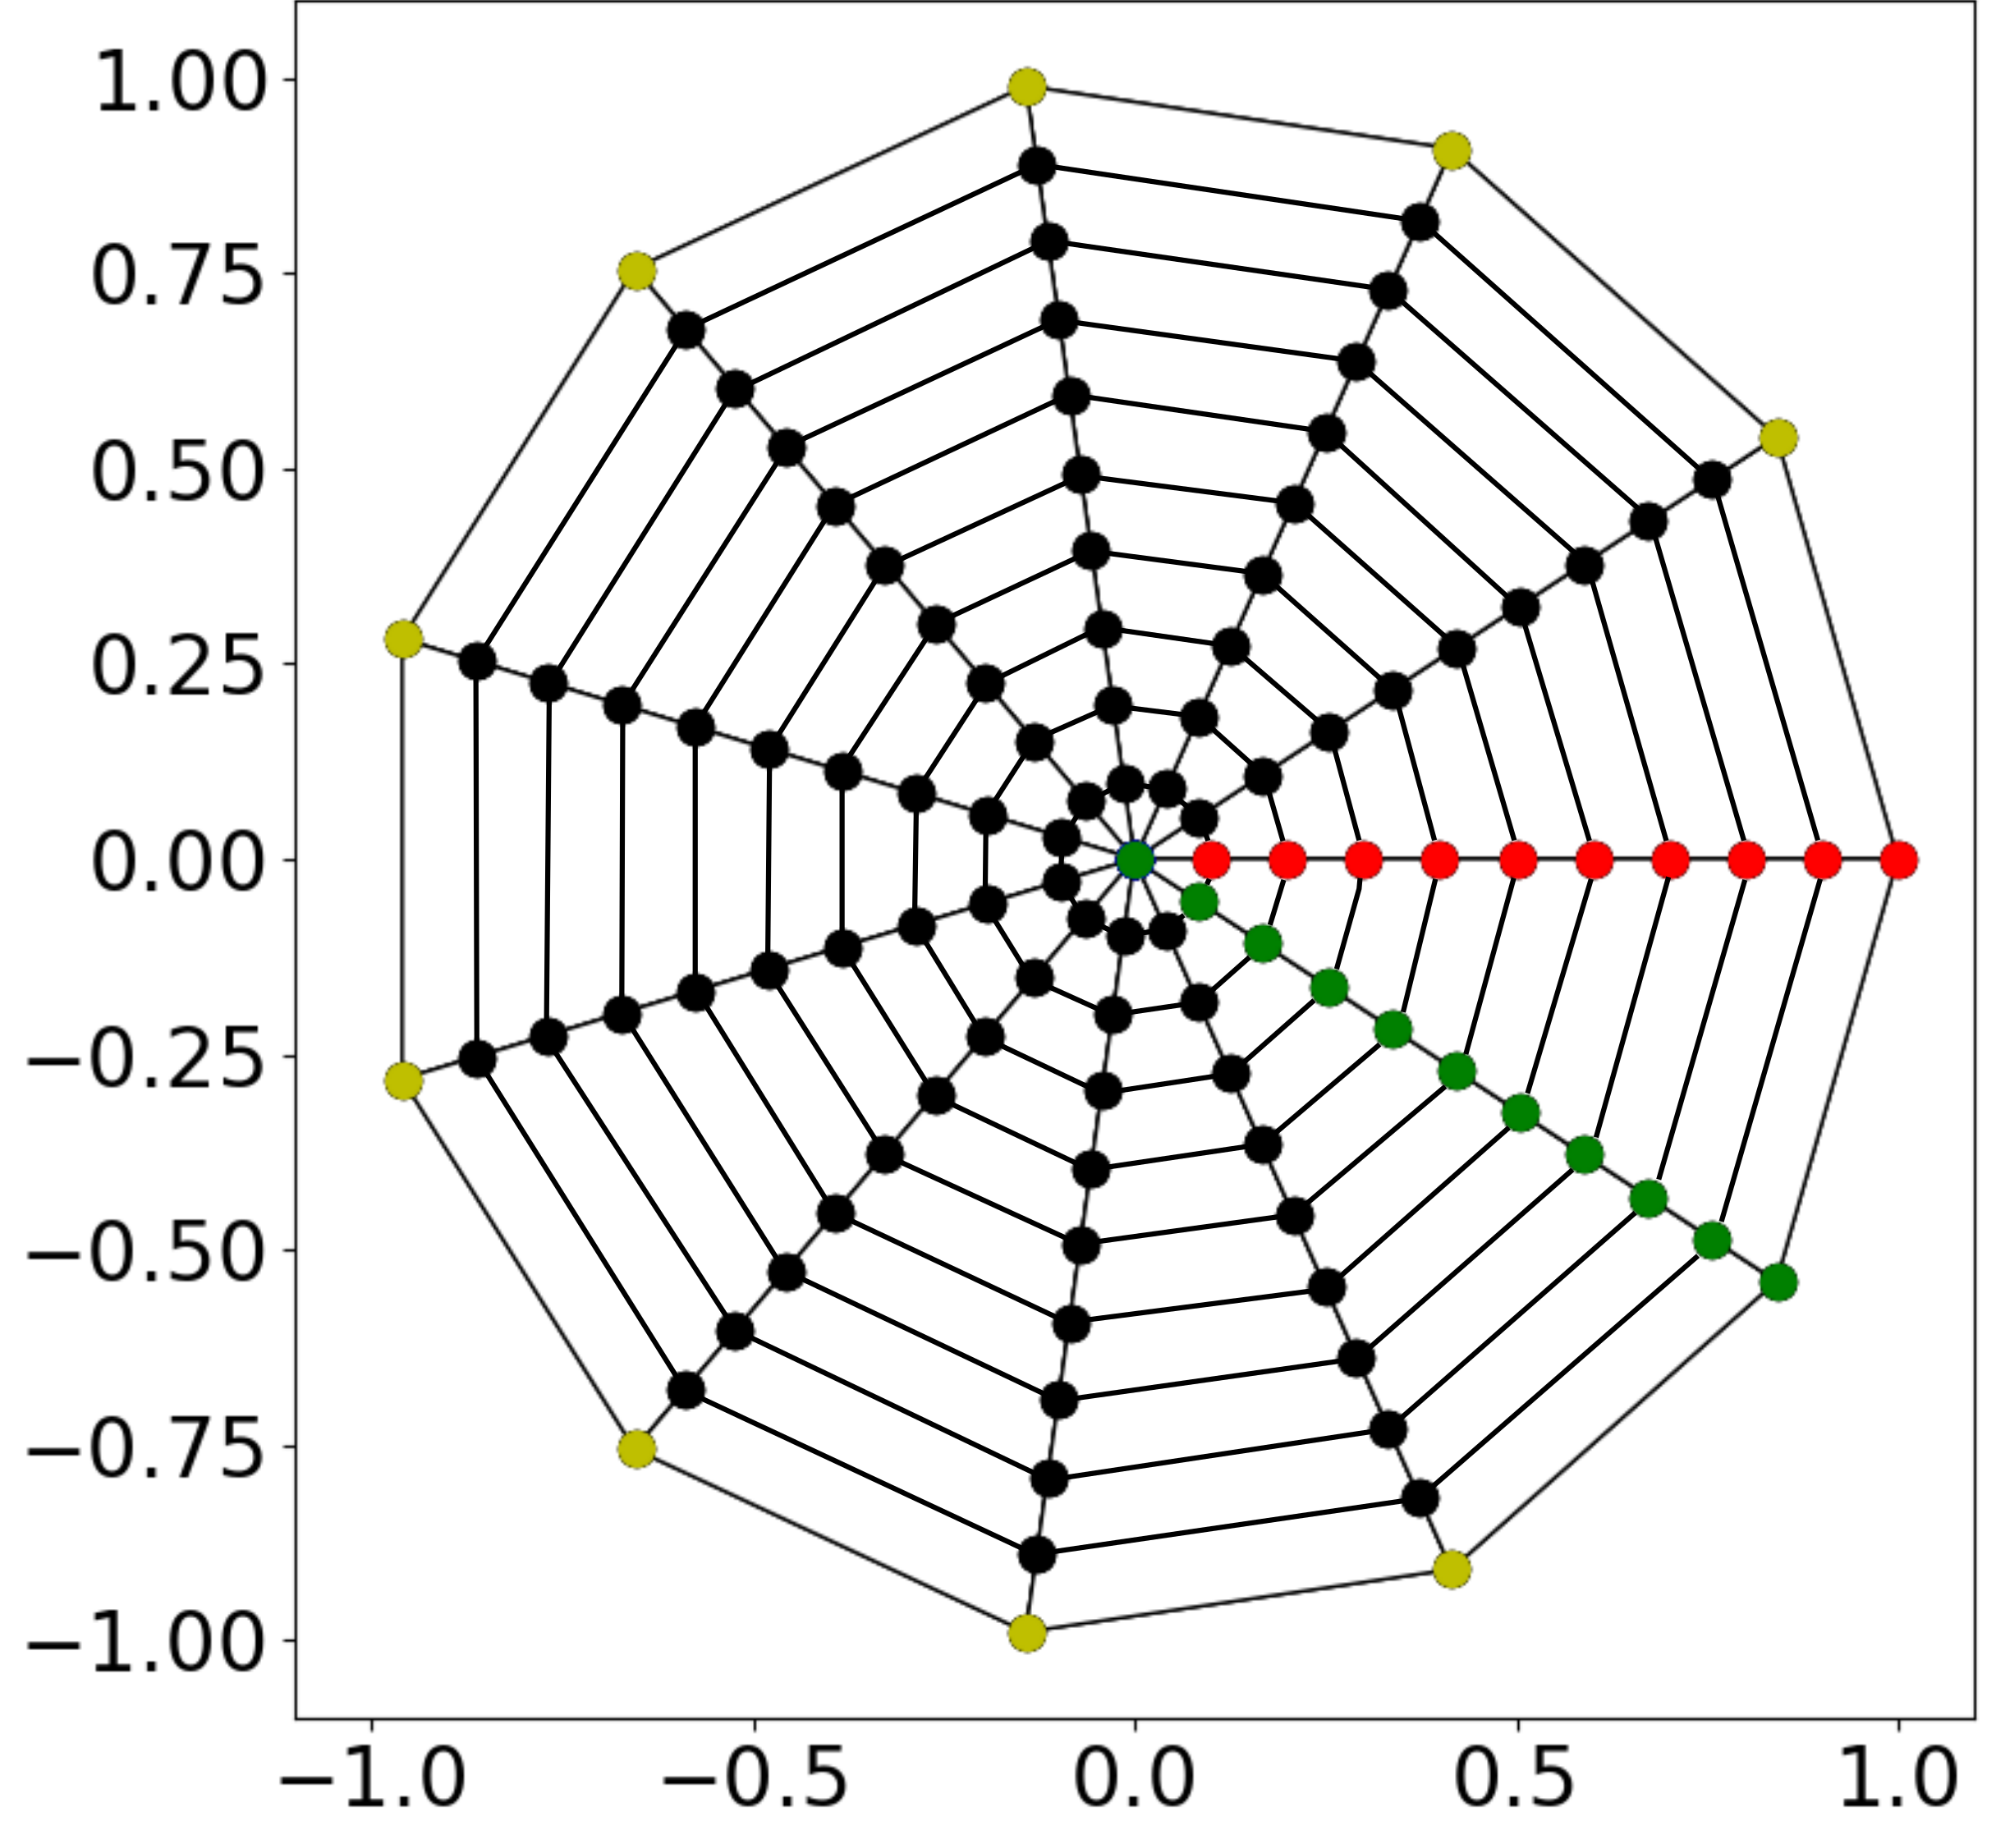
\includegraphics[width=\textwidth]{images/fiber_creation/quad_0.png}%
    \caption{Unit circle, scheme 1}%
    \label{fig:quad_0}%
  \end{subfigure}
  \quad
  \begin{subfigure}[t]{0.48\textwidth}%
    \centering%
    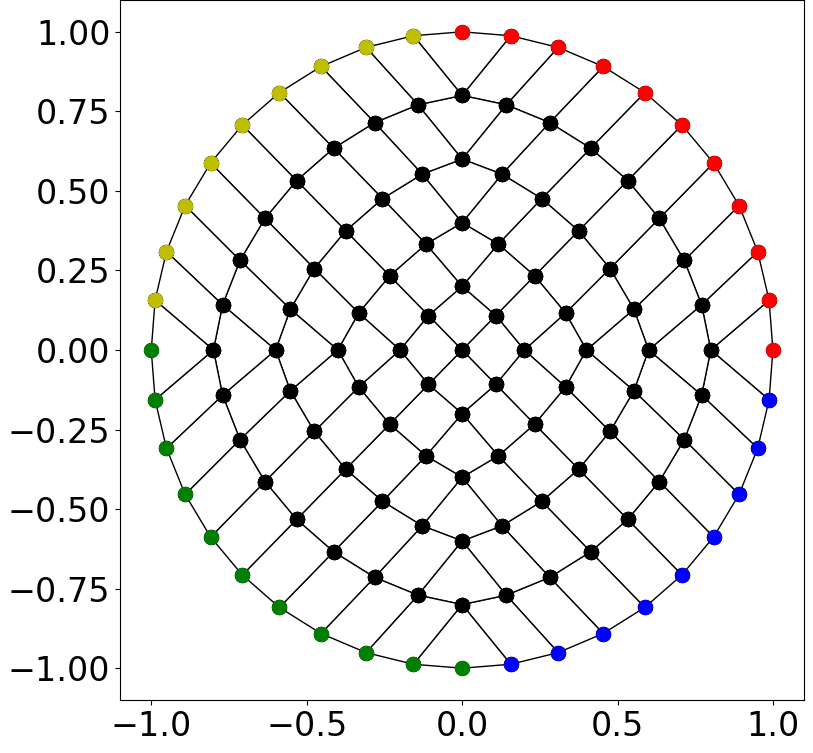
\includegraphics[width=\textwidth]{images/fiber_creation/quad_3.png}%
    \caption{Unit circle, scheme 2}%
    \label{fig:quad_3}%
  \end{subfigure}
  \caption{Four different quadrangulation schemes of the parameter domain with $11\times 11$ nodes. The boundaries of the grid are colored for better perceptiblity. In (a) and (b), the parameter domain is a unit square with a uniform grid (a) and an adjusted grid (b) that tries to reduce the problem of degenerate elements at the corners of the muscle slices. In (c) and (d), quadrangulations on a unit circle parameter domain are shown. (c) shows a rotationally symmetric construction scheme whereas the approach in (d) is similar to a uniform grid.}%
  \label{fig:quads}%
\end{figure}%

Next, the grid in the parameter domain is transferred to the muscle domain by applying the harmonic map $\bfy(\bfx) \in S_M$ on every point of the quadrangulation $\bfx \in \Omega_P$. This is illustrated in \cref{fig:serial_alg_4} for a parameter domain consisting of the unit circle, with quadrangulation scheme 2 and $5 \times 5$ nodes. The cells of the grid in $\Omega_P$ are shown in the right-most stack of domains. The grid points are visualized left of the grids. The resulting image of the mesh in the slices $S_M$ is shown on the left. For visualization reasons, each quadrilateral has been split into two triangles.

\subsection{Formation of Three-Dimensional Elements}

The result of the previous steps is a number of quadrangulated muscle slices. The grid on every slice has the same number of nodes and elements. The nodes on the boundary of neighboring slices are positioned similarly.

The final step of \cref{alg:serial_algorithm_1} is line \ref{alg:1.5}, the formation of 3D elements. Inserting vertical edges between all corresponding nodes on two neighboring slices creates a set of 3D hexahedral elements and, thus, an overall 3D hexahedral mesh of the muscle volume. This step is visualized in \cref{fig:serial_alg_8}.

\subsection{Generation of Fiber Meshes}\label{sec:generation_of_fiber_meshes}

1D fiber meshes are created following the approach of computing a divergence free vector field introduced in \cite{Choi2013}. The steps are given in \cref{alg:serial_algorithm_2}.

The Laplace problem to be solved can be stated as%
\begin{align}\label{eq:fiberest_laplace}
  Δp(\bfx) = 0 \quad \text{for } \bfx \in \Omega_M.
\end{align}
The vector field is given by the gradient $\nabla p$ of a solution $p$ of \cref{eq:fiberest_laplace}. The quantities can be interpreted as pressure $p$ and (negative) velocity field $\nabla p$ of a steady flow.
The muscle fibers are given as streamlines or, equivalently, pathlines in this velocity field. Every streamline $\bfx : [-c_1,c_2] \subset \R \to \Omega_M$ with $c_1,c_2 > 0$ is defined by a seed point $\bfx_0$ and the property that it is tangent to the velocity field at any point:
\begin{align*}
  \bfx(0) = \bfx_0,\quad
  \p{\bfx(s)}{s} = \nabla p\big(\bfx(s)\big).
\end{align*}

As proposed by \cite{Choi2013}, Neumann boundary conditions can be specified for the bottom and top surfaces of the muscle volume, $∂\Omega_{M, \text{bottom}}$ and $∂\Omega_{M, \text{top}}$:
\begin{equation}\label{eq:fiberest_neumann}
\begin{array}{rlrlr}
  \d{p(\bfx)}{\bfx} \cdot \bfn &= F_\text{in}, \quad &&\text{for } \bfx \in ∂\Omega_{M, \text{bottom}},\\[4mm]
  \d{p(\bfx)}{\bfx} \cdot \bfn &= F_\text{out}, \quad &&\text{for } \bfx \in ∂\Omega_{M, \text{top}}.
\end{array}
\end{equation}
The in and outflow values $F_\text{in}<0$ and $F_\text{out}>0$ are balanced such that the total inflow ${F_\text{in}\cdot \mu(∂\Omega_{M, \text{bottom}})}$ compensates the total outflow ${F_\text{in}\cdot \mu(∂\Omega_{M, \text{bottom}})}$. Here, $\mu(∂\Omega)$ is the surface area of the respective boundary.

Alternatively, Dirichlet boundary conditions can be specified:
\begin{equation}\label{eq:fiberest_dirichlet}
\begin{array}{rlrlr}
  p(\bfx) &= 0, \quad &&\text{for } \bfx \in ∂\Omega_{M, \text{bottom}},\\[4mm]
  p(\bfx) &= 1, \quad &&\text{for } \bfx \in ∂\Omega_{M, \text{top}}.
\end{array}
\end{equation}
The specification of Dirichlet boundary conditions has the same effect as Neumann boundary conditions and is easier to define. The in and outflows are still orthogonal to the boundary because the prescribed value of $p$ does not vary in the planar boundary.

The boundary value problem given by \cref{eq:fiberest_laplace,eq:fiberest_neumann}  or \cref{eq:fiberest_laplace,eq:fiberest_dirichlet} is discretized by the finite element method with linear or quadratic ansatz functions and solved by our software \opendihu{} using the 3D mesh generated from \cref{alg:serial_algorithm_1}. The divergence free gradient field is visualized in \cref{fig:potential_flow}. The gradient values are directly given by the finite element discretization. The gradient is elementwise constant for linear ansatz functions and trilinear for quadratic ansatz functions.

The next step in \cref{alg:serial_algorithm_2} is line \ref{line:2.3}, tracing streamlines through the gradient field. Seed points are selected on the 2D cross section at the vertical center of the 3D muscle domain. The seed points are sampled regularly on the square or circular parameter domain according to the quadrangulation scheme and then mapped to the respective muscle slice.
Because the 3D mesh was created using harmonic maps, the resulting spacing between the seed points is very uniform.

For the tracing of streamlines, the semi-analytical Pollock's method \cite{Pollock1988} is often used, which was originally developed for fixed 2D finite difference grids. Extensions to irregular 3D grids and for given velocities at nodes instead of fluxes over faces have been formulated \cite{HAEGLAND2007Streamline}. Other, more accurate algorithms exist \cite{cordes1992continuous}, including higher order formulations \cite{juanes2006unified}.

Because modeling muscle fascicles is only a heuristic approach, the generated streamlines do not have to be exceptionally accurate. Therefore, we use a fully numerical method. The streamlines are generated by explicit Euler integration of the gradient vectors in top and bottom direction. A small spatial step width of $h=\num{1e-2}$ is used. Details of the algorithm are given in the next section, \cref{sec:algorithm_for_streamline_tracing}. In line \ref{line:2.4} of \cref{alg:serial_algorithm_2}, all generated streamlines are resampled to obtain the desired widths of the 1D elements.
\Cref{fig:fiber_tracing_streamlines} visualizes the resulting streamlines in the biceps muscle.

\begin{algorithm}
  \begin{algorithmic}[1]%
    \Statex\Procedure{Create\_1D\_meshes}{}
    \Require Structured 3D volume mesh
    \Ensure 1D fiber meshes
    \Statex
    \State Solve Laplacian flow problem   \label{line:2.2}
    \State Trace streamlines in the gradient field  \label{line:2.3}
    \State Resample 1D fiber meshes \label{line:2.4}
    \EndProcedure
  \end{algorithmic}%
  \caption{Serial algorithm}%
  \label{alg:serial_algorithm_2}%
\end{algorithm}%

\begin{figure}%
  \centering%
  \begin{subfigure}[t]{0.48\textwidth}%
    \centering%
    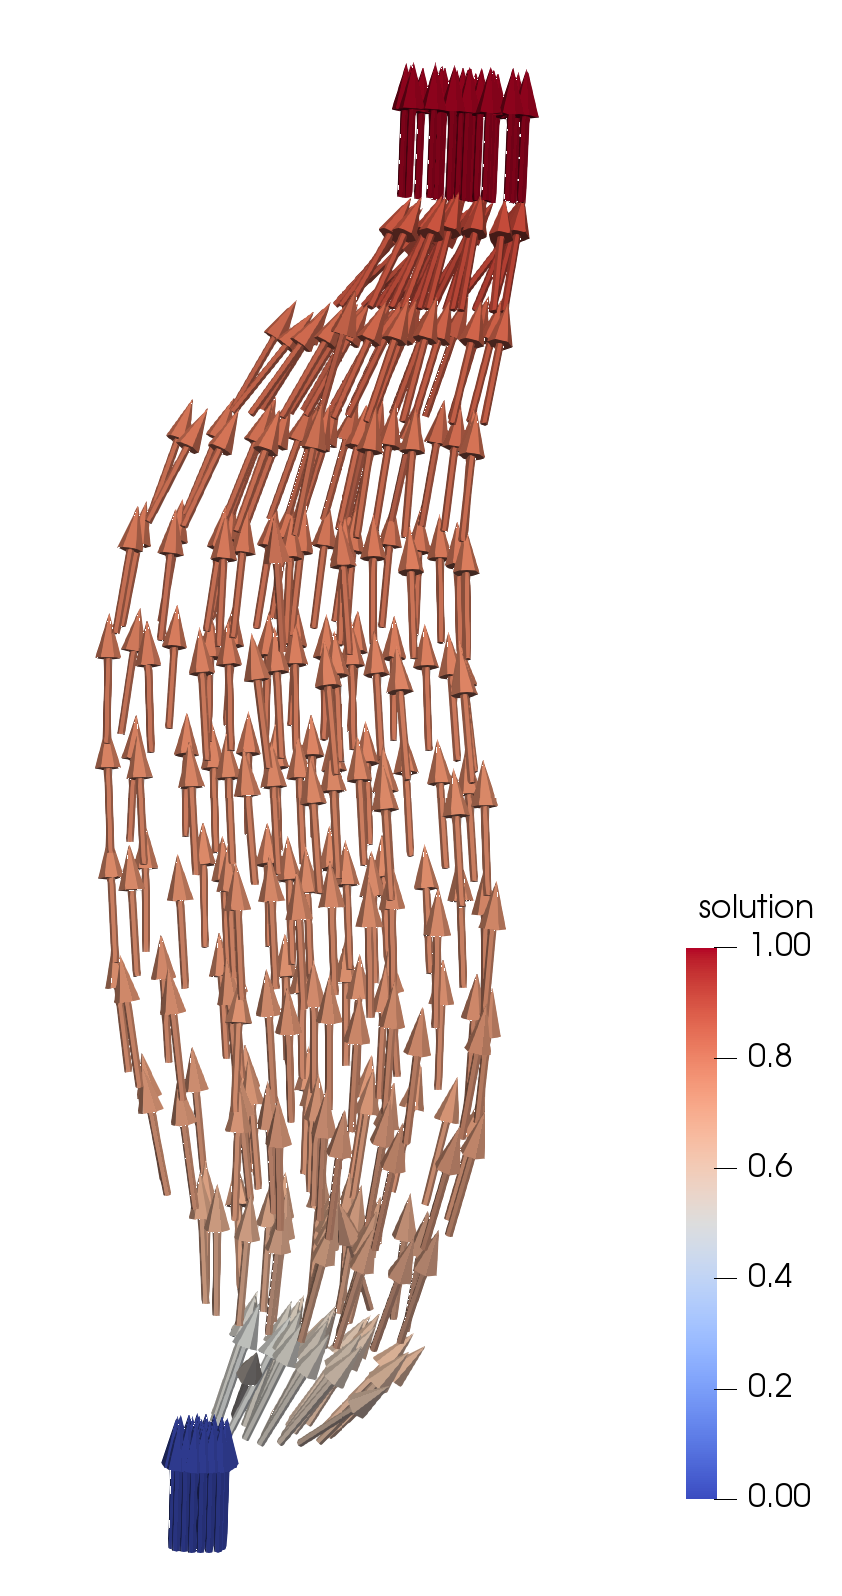
\includegraphics[height=10cm]{images/fiber_creation/potential_flow.png}%
    \caption{Solution (color coding) and direction vectors of the gradient field for the boundary value problem \cref{eq:fiberest_laplace} with Dirichlet boundary conditions \cref{eq:fiberest_dirichlet}.}%
    \label{fig:potential_flow}%
  \end{subfigure}
  \quad
  \begin{subfigure}[t]{0.48\textwidth}%
    \centering%
    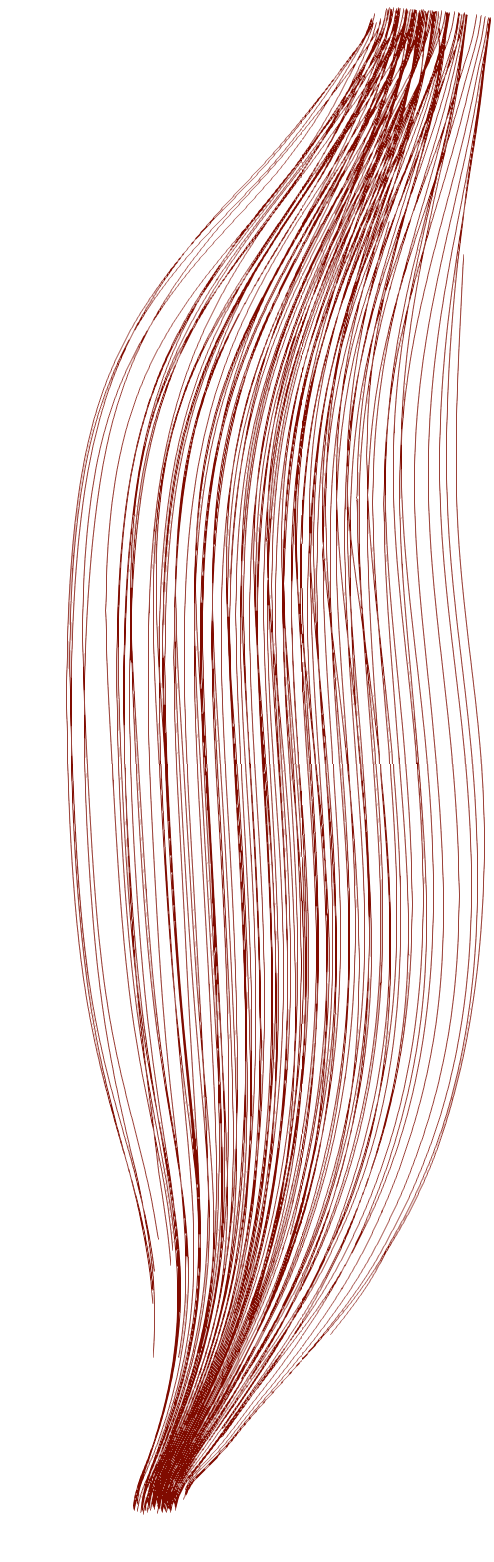
\includegraphics[height=10cm]{images/fiber_creation/streamlines_red.png}%
    \caption{Resulting streamlines that were traced through the gradient field.}%
    \label{fig:fiber_tracing_streamlines}%
  \end{subfigure}
  \caption{Setup and solution of the Laplace problem for the biceps geometry that is used to estimate muscle fibers by streamline tracing.}%
  \label{fig:potential_flow_streamlines}%
\end{figure}%

\subsection{Algorithm for Streamline Tracing}\label{sec:algorithm_for_streamline_tracing}
The algorithm for streamline tracing uses an efficient method to traverse the mesh, which makes use of its structuredness.
At first, the element $E^{(0)}$ in the mesh that contains the first seed point $\bfp^0$ needs to be found. By construction of the mesh generation algorithms, this is always the element with the lowest index. 
However, if the seed point is not found there, the scheme is robust enough to search in all other elements.

Starting from the seed point $\bfp^0 = \bfp^{(i)}$ in element $E^{(i)}$, the next point $\bfp^{(i+1)}$ of a streamline is computed as %
\begin{align*}
  \bfp^{(i+1)} = \bfp^{(i)} + h\,\nabla p (\bfp^{(i)}).
\end{align*}
After $\bfp^{(i+1)}$ has been computed, the mesh element $E^{(i+1)}$ where it is located needs to be identified. This is needed to evaluate the gradient value $\nabla p (\bfp^{(i+1)})$ at the new point by interpolation according to the FE representation of $p$.

At first, the element $E^{(i)}$ of $\bfp^{(i)}$ is checked whether it also contains $\bfp^{(i+1)}$. If not, the neighboring element in the direction of the streamline is considered. This neighboring element is chosen among all up to 26 possible neighbors such that the direction from the previous element $E^{(i-1)}$ to the current element $E^{(i)}$ continues.

If this element is also not the right one, all other neighbors of $E^{(i)}$ are subsequently checked, ordered by their plausibility according to the previous streamline direction. If none of the 27 considered elements contains the computed point, a search among all elements of the entire mesh is performed. This case happens only for unsuited choices of the integration width $h$, i.e., if the streamline tracing skips whole elements.

The end of a streamline is detected when the streamline reaches the final $z$ plane, either at the bottom or top of the muscle volume. To make the algorithm more robust, also the case is considered where the streamline leaves the muscle domain to the side shortly before reaching the end of the muscle. This can happen due to discretization errors for streamlines that start close to the boundary of the muscle. In such a case, the missing rest of the streamline is interpolated from up to four existing neighboring parallel streamlines.

After the end of the streamline is found, tracing of the next streamline starts at the next seed point $\bfp^0_\text{next}$. The element where $\bfp^0_\text{next}$ is located can also be easily determined in the structured mesh.

The presented scheme avoids repeatedly traversing all elements of the mesh by predicting the next elements according to streamline direction and organization of seed points. This is facilitated by the structured mesh, which has well-defined element neighbor relations.
At the same time, the scheme is robust enough to also efficiently handle streamlines in other use cases. It can also be reused, e.g., in muscle fiber tracing applications of more complex shaped muscles where the fibers change directions.

\subsection{Results and Discussion}\label{sec:mesh_generation_0_results_and_discussion}
The presented \cref{alg:serial_algorithm_1,alg:serial_algorithm_2} generate a 3D mesh and 1D muscle fibers from a triangulated surface. Three different triangulation strategies for the slices and four different reference quadrangulations can be chosen. In the following, the different choices are evaluated.

The different triangulation methods for the slices discussed in \cref{sec:triangulation_of_the_slices} are visualized in the three columns of \cref{fig:tri_triangulations}. 
The top rows show the triangulation of $S_M$ and the harmonic map $u$ as color coded values from violet to yellow. $u$ is the horizontal coordinate on the reference domain. A point with violet color in $S_M$ will be mapped to the left-most point in the parameter space $\Omega_P$. Similarly, a yellow point will be mapped to a point far at the right in $\Omega_P$.

The middle and bottom rows in \cref{fig:tri_triangulations} show the image of the triangulation in $\Omega_P$ under the harmonic map, for the unit square and the unit circle, respectively. The mapping between the colored boundary points stems from the Dirichlet boundary conditions in the formulation of the harmonic map. In consequence, the boundary points are by construction equally spaced both in the muscle domain $S_M$ and in the parameter domain $\Omega_P$.

It can be seen that the triangulation appears distorted in the parameter domain. The effect is most significant for the square in \cref{fig:triu_1} and \cref{fig:triu_2}. For the latter, the center point of the muscle domain $S_M$ gets mapped far off the center of the squared parameter domain. This effect does not occur for the circle.

The reason for this lies in the triangulation of $S_M$ together with the boundary shape. In the third method, only the value at the center point is a degree of freedom in the computation of $u$ while the values at the boundary points are fixed. By the triangulation, the value of $u$ varies linearly from the boundary towards the center point.
By comparing the colored boundary points in the muscle slice in the top row with the square in the second row, it can be seen that the prescribed values for $u$ are 0 at all blue points, 1 at all yellow points and linearly increasing from 0 to 1 at the green and red points, increasing from left to right.
The yellow points of $S_M$ with the prescribed constant value of $u=1$ are approximately located on a vertical line. The first two derivatives of $u$ in vertical coordinate direction are therefore almost zero, in consequence, the Laplace equation forces the derivatives in horizontal direction to also be approximately zero. Therefore, the solution value at the center point is close to $1$. This leads to the mapped center point being close to the right boundary in the square parameter domain. The same happens for the vertical coordinate $v$ of the harmonic map.

For the circle, neighboring boundary points are not located on horizontal or vertical lines and, thus, the Dirichlet bondary conditions for $u$ and $v$ vary along the boundary. Therefore, a better mapping is obtained. The shape of the muscular slice is more similar to the circle than to the square.

Another result that can be seen in \cref{fig:tri_triangulations} is the effect of the failure of the first method to handle concave slices on the harmonic map. As the top left image shows, the first triangulation method produces triangles outside the domain. The triangles are located around the red boundary points. In the square parameter domain, these triangles are degenerated and lie on the bottom boundary. In the circle parameter domain where the respective triangles can be seen at the bottom, they even intersect other triangles. This yields an invalid triangulation.

The reasons for degenerate triangles in the square parameter domains are not solely the concave muscle slices. Also, the straight sides of the unit square lead to degenerate triangles whenever three boundary points of the same side form a triangle.
In the example in \cref{fig:tri_triangulations}, this occurs for the square in column (\subref{fig:triu_0}). As can be seen in the triangulated slice in the top row, there are three triangles that are entirely made up of blue boundary points. These triangles get mapped onto the left side of the square parameter domain where they have a vanishing surface area.

The same effect also occurs with the second triangulation method in column (\subref{fig:triu_1}) of \cref{fig:tri_triangulations} where a triangle at the bottom right is comprised of three red boundary points and, therefore, gets mapped to the bottom side of the square. Because of the guaranteed minimum angle in the second triangulation method, this circumstance occurs less often and only for muscle cross sections where the boundary makes sharp turns, such as the muscle slice in this example. The third triangulation method is guaranteed to avoid this problem as all triangles are connected with the center point.

% ------------------
% parameter space triangulations
\begin{figure}%
  \centering%
  \begin{subfigure}[t]{0.31\textwidth}%
    \centering%
    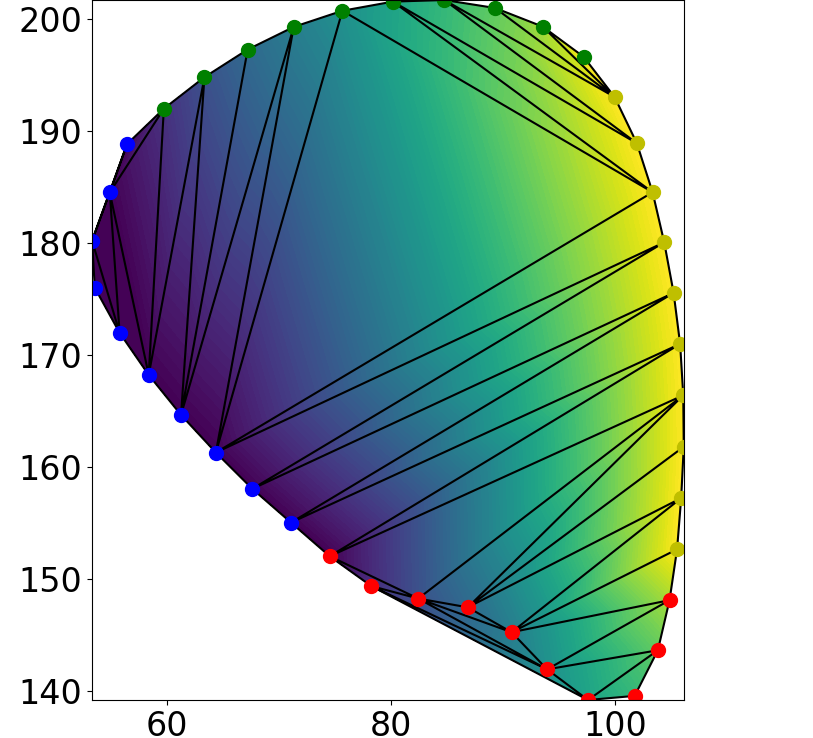
\includegraphics[width=\textwidth]{images/fiber_creation/u_0.png}%
    \caption{First method,\\Quickhull agorithm}%
    \label{fig:triu_0}%
  \end{subfigure}
  \quad
  \begin{subfigure}[t]{0.31\textwidth}%
    \centering%
    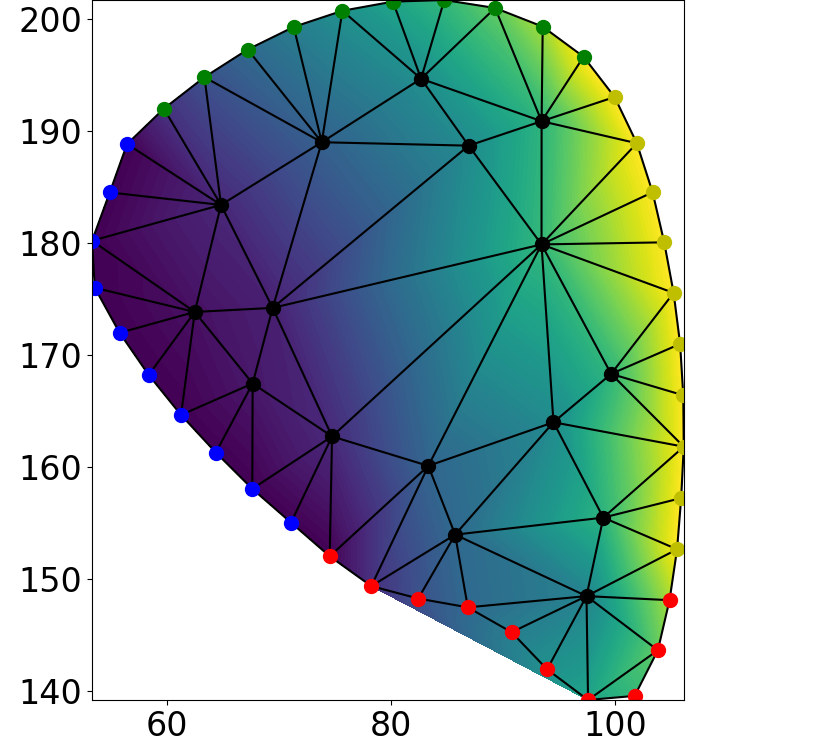
\includegraphics[width=\textwidth]{images/fiber_creation/u_1.png}%
    \caption{Second method,\\Delaunay refinement}%
    \label{fig:triu_1}%
  \end{subfigure}
  \quad
  \begin{subfigure}[t]{0.31\textwidth}%
    \centering%
    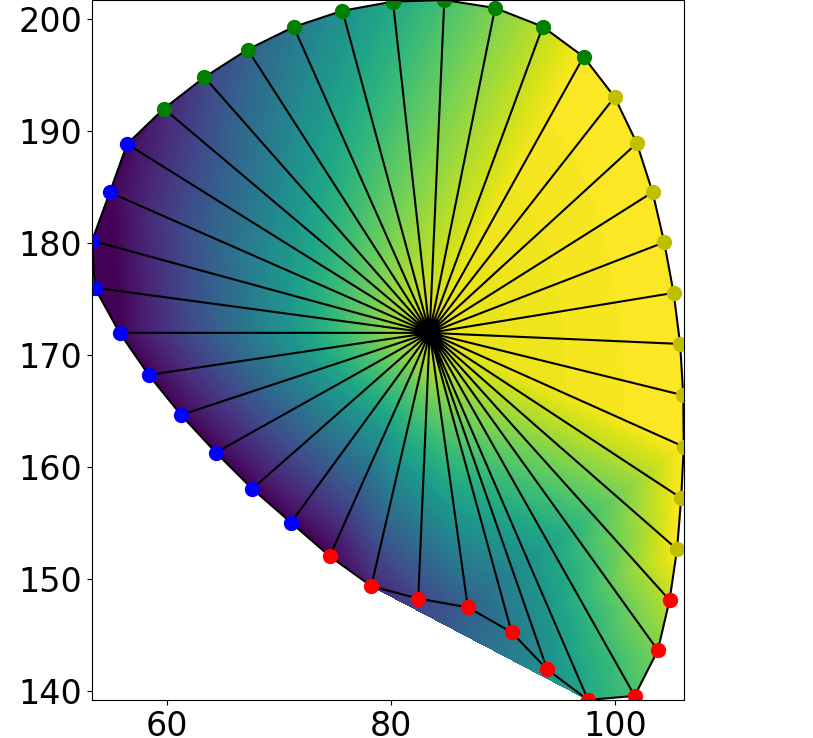
\includegraphics[width=\textwidth]{images/fiber_creation/u_2.png}%
    \caption{Third method,\\center of gravity}%
    \label{fig:triu_2}%
  \end{subfigure}\\
  
  % square
  \begin{subfigure}[t]{0.31\textwidth}%
    \centering%
    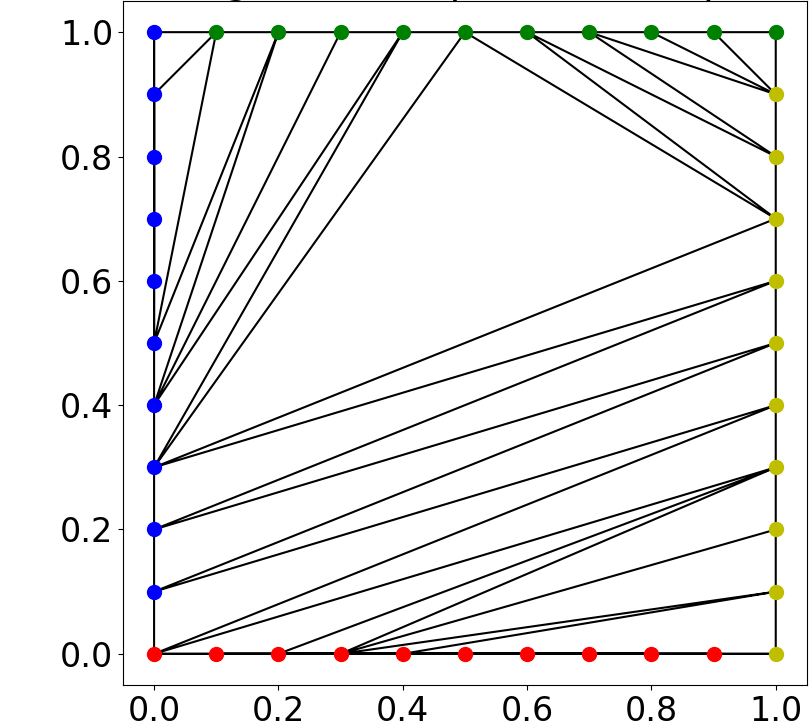
\includegraphics[width=0.9\textwidth, trim=37mm 14mm 6mm 6mm, clip]{images/fiber_creation/mesh_plots/out_0_1_0_tri.png}%
    %\caption{}%
    \label{fig:w_01}%
  \end{subfigure}
  \quad
  \begin{subfigure}[t]{0.31\textwidth}%
    \centering%
    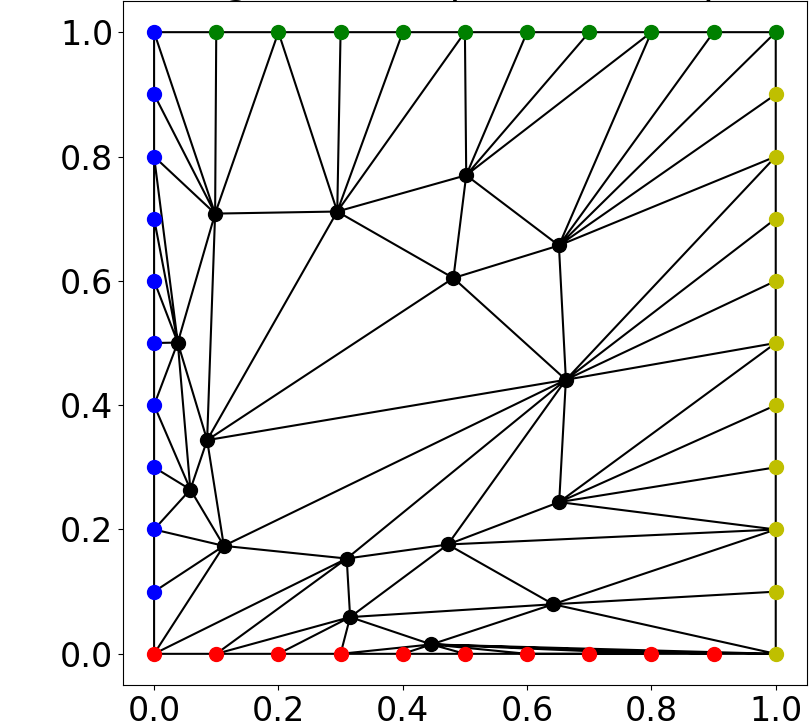
\includegraphics[width=0.9\textwidth, trim=37mm 14mm 6mm 6mm, clip]{images/fiber_creation/mesh_plots/out_1_1_0_tri.png}%
    %\caption{}%
    \label{fig:w_11}%
  \end{subfigure}
  \quad
  \begin{subfigure}[t]{0.31\textwidth}%
    \centering%
    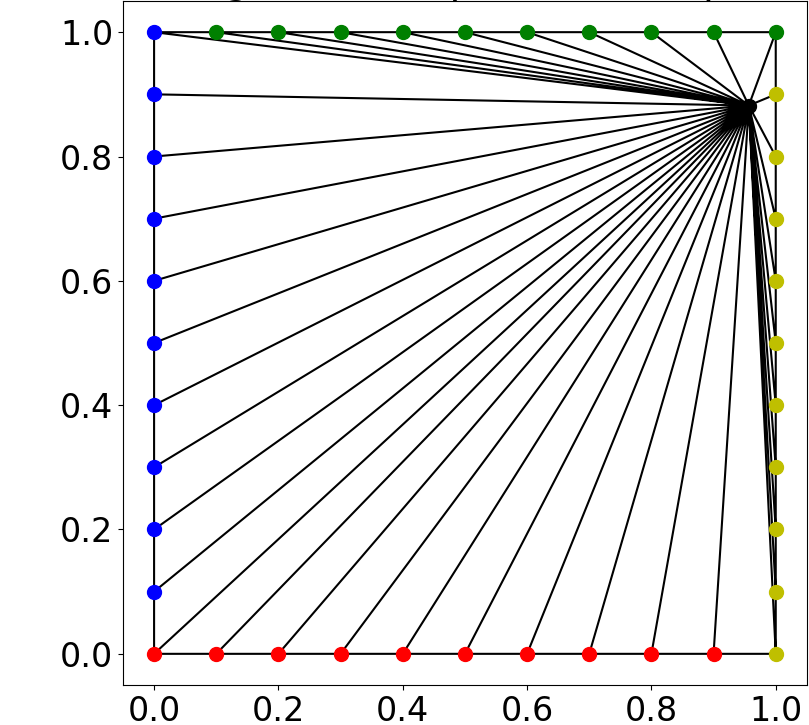
\includegraphics[width=0.9\textwidth, trim=37mm 14mm 6mm 6mm, clip]{images/fiber_creation/mesh_plots/out_2_1_0_tri.png}%
    %\caption{}%
    \label{fig:w_21}%
  \end{subfigure}\\
  
  % circle
  \hspace{-12mm}
  \begin{subfigure}[t]{0.31\textwidth}%
    \centering%
    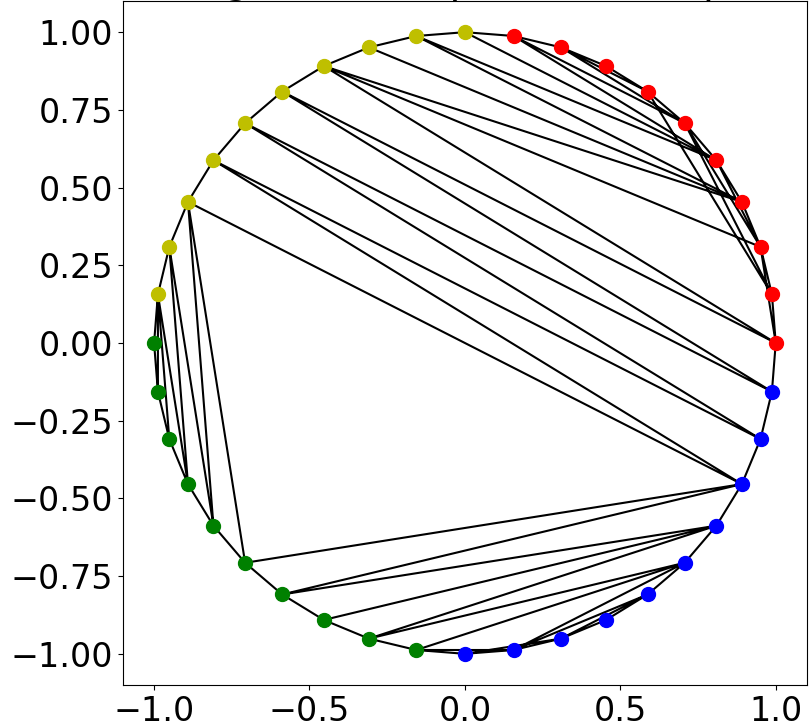
\includegraphics[width=0.9\textwidth, trim=37mm 14mm 6mm 6mm, clip, angle=225,origin=c]{images/fiber_creation/mesh_plots/out_0_0_0_tri.png}% trim=left bottom right top, clip]
    %\caption{}%
    \label{fig:w_00}%
  \end{subfigure}
  \quad
  \begin{subfigure}[t]{0.31\textwidth}%
    \centering%
    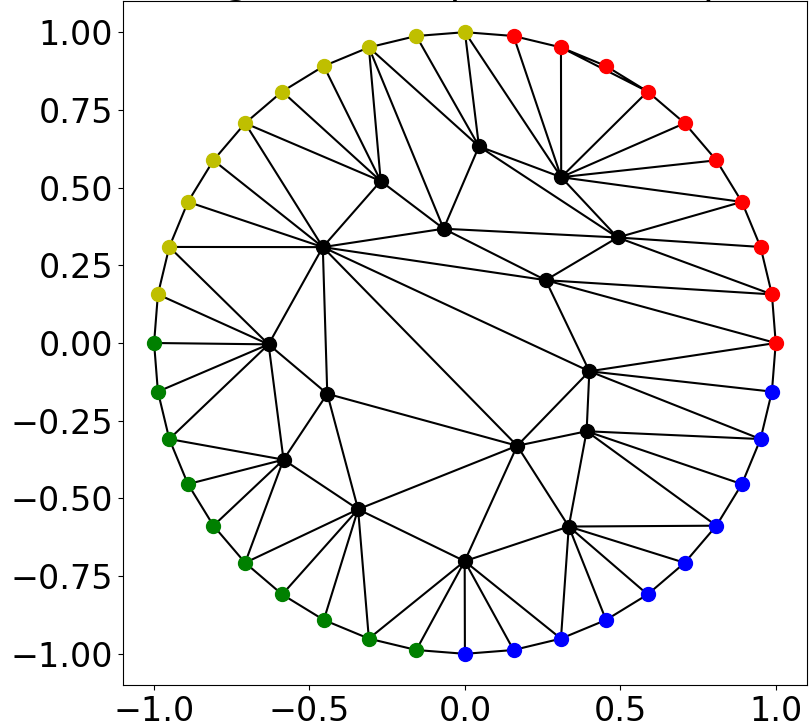
\includegraphics[width=0.9\textwidth, trim=37mm 14mm 6mm 6mm, clip, angle=225,origin=c]{images/fiber_creation/mesh_plots/out_1_0_0_tri.png}%
    %\caption{}%
    \label{fig:w_10}%
  \end{subfigure}
  \quad
  \begin{subfigure}[t]{0.31\textwidth}%
    \centering%
    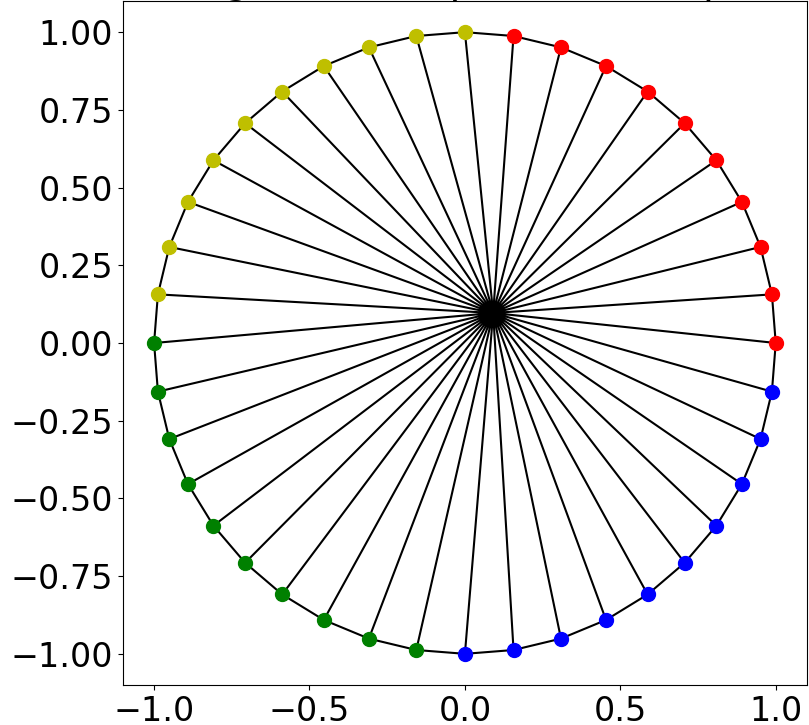
\includegraphics[width=0.9\textwidth, trim=37mm 14mm 6mm 6mm, clip, angle=225,origin=c]{images/fiber_creation/mesh_plots/out_2_0_0_tri.png}%
    %\caption{}%
    \label{fig:w_20}%
  \end{subfigure}
  
  \caption{Initial slice triangulation and harmonic maps in 3D mesh generation: Top row: Different triangulation methods for $S_M$, the color represents the solution $u$ of the harmonic map. Middle and bottom row: triangulation mapped to the parameter domain $\Omega_P$, for the unit square (middle) and the unit circle (bottom). Each column corresponds to one triangulation method.}%
  \label{fig:tri_triangulations}%
\end{figure}%

In conclusion, the second triangulation method with the unit circle and the third triangulation method with both unit square and unit circle show good behavior for use in our meshing algorithm. Next, their interplay with the quadrangulation of the parameter space needs to be investigated.

% bis hierher Änderungen eingearbeitet

In the next step, the algorithm creates a quadrilateral mesh in the parameter domain and computes its image in the muscle domain using the inverse of the harmonic map. The results are shown in \cref{fig:tri_meshes} for the three different initial triangulation methods (columns) and the four different schemes to create the quadrilateral mesh (rows).

In the images in column (\subref{fig:tu_2}) and rows (\subref{fig:tquad_1}) and (\subref{fig:tquad_2}), it can be seen that the previously observed effect of a bad mapping for squares and the third triangulation method also leads to a mesh in $S_M$ of poor quality.
The result for the two square schemes in column (\subref{fig:tu_1}) is better but still not satisfactory. Good results with the square reference domain are only observed for the first triangulation method in this example.

It can be seen that the approximation quality of the boundary of the domain varies. Most of all, the combination of the first triangulation method (column (\subref{fig:tu_0})) and the square parameter domain (rows (\subref{fig:tquad_1}) and (\subref{fig:tquad_2})) reproduces the shape of the slice poorly. 
The mismatch occurs at the blue and red boundary points. Additionally, the second triangulation method (column (\subref{fig:tu_1})) for the squares fails to correctly represent the round boundary at the bottom of the domain.
The degenerate triangles in the parameter domain are the cause for this effect. The harmonic map $\bfy: S_M \to \Omega_P$ is not injective and, therefore, its inverse does not exist. In our implementation, the points on the degenerate triangles in $\Omega_P$ are mapped to an arbitrarily selected location inside the corresponding triangles in $S_M$. Thus, the mapping is correctly inverted at locations of valid triangles and only creates different boundary points in the invalid areas.


Furthermore, it can be seen that an inaccurate representation of the boundary also occurs with the parameter mesh in the unit circle generated by scheme 1. In this case, the reason is the low number of elements at the boundary in the parameter domain quadrangulation.

The two schemes for the circle parameter domain in rows (\subref{fig:tquad_0}) and (\subref{fig:lquad_3}) both generate reasonable meshes for all triangulation methods, despite the different structure of the generated meshes. The best results for both schemes have been obtained with the third triangulation method.

% ------------------
% resulting meshes
\begin{figure}%
  \centering%
  \hspace{0.24\textwidth}
  \begin{subfigure}[t]{0.24\textwidth}%
    \centering%
    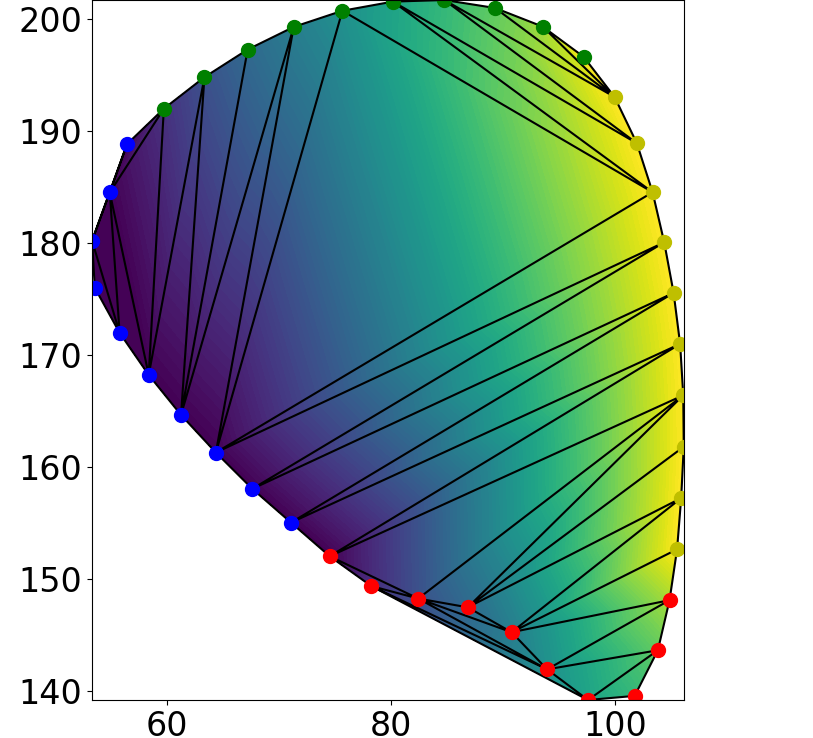
\includegraphics[width=\textwidth]{images/fiber_creation/u_0.png}%
    \caption{First method}%
    \label{fig:tu_0}%
  \end{subfigure}
  \begin{subfigure}[t]{0.24\textwidth}%
    \centering%
    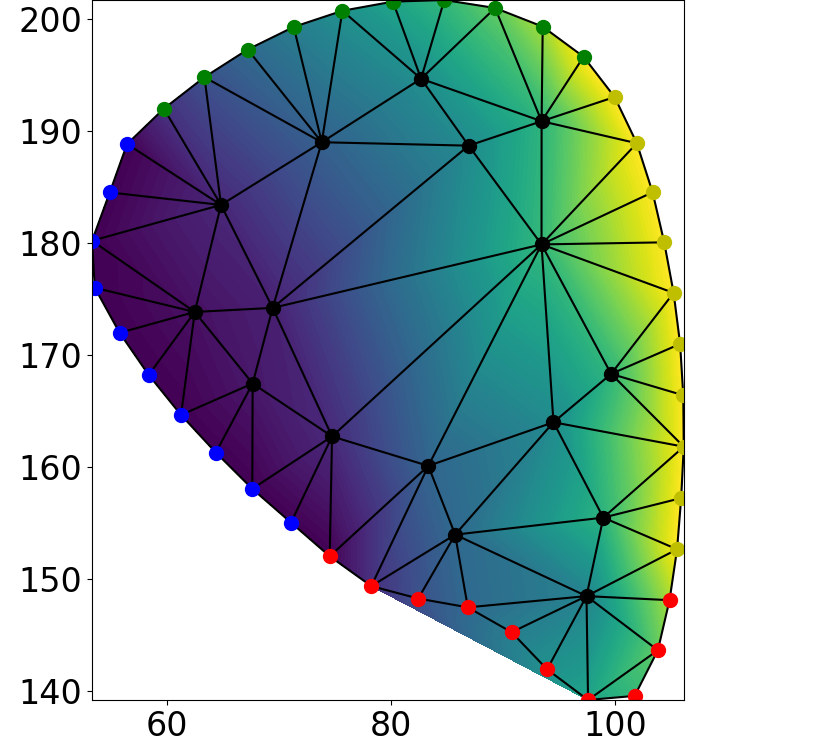
\includegraphics[width=\textwidth]{images/fiber_creation/u_1.png}%
    \caption{Second method}%
    \label{fig:tu_1}%
  \end{subfigure}
  \begin{subfigure}[t]{0.24\textwidth}%
    \centering%
    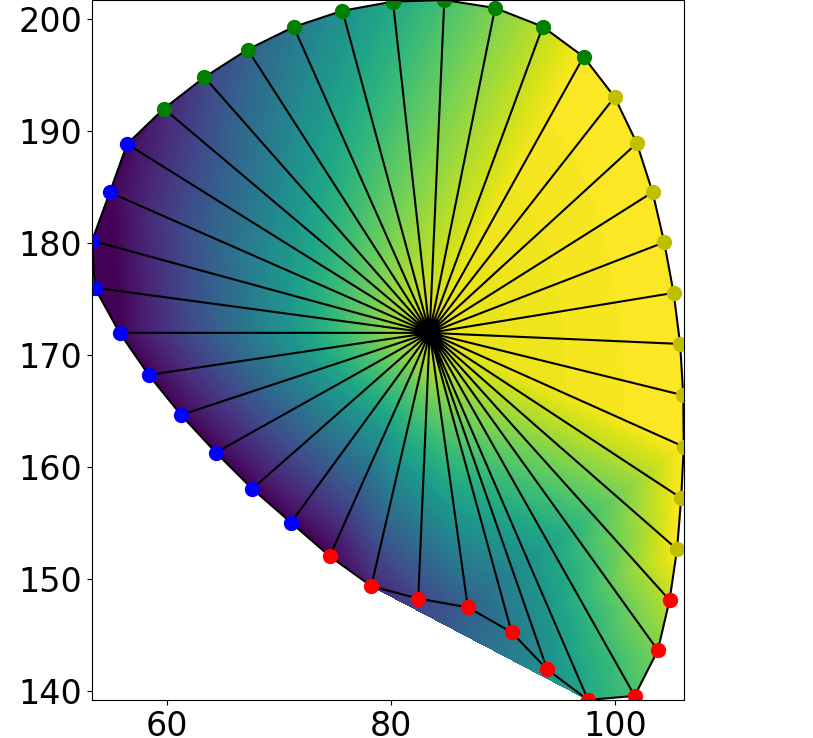
\includegraphics[width=\textwidth]{images/fiber_creation/u_2.png}%
    \caption{Third method}%
    \label{fig:tu_2}%
  \end{subfigure}\\
  
  % square
  \begin{subfigure}[t]{0.24\textwidth}%
    \centering%
    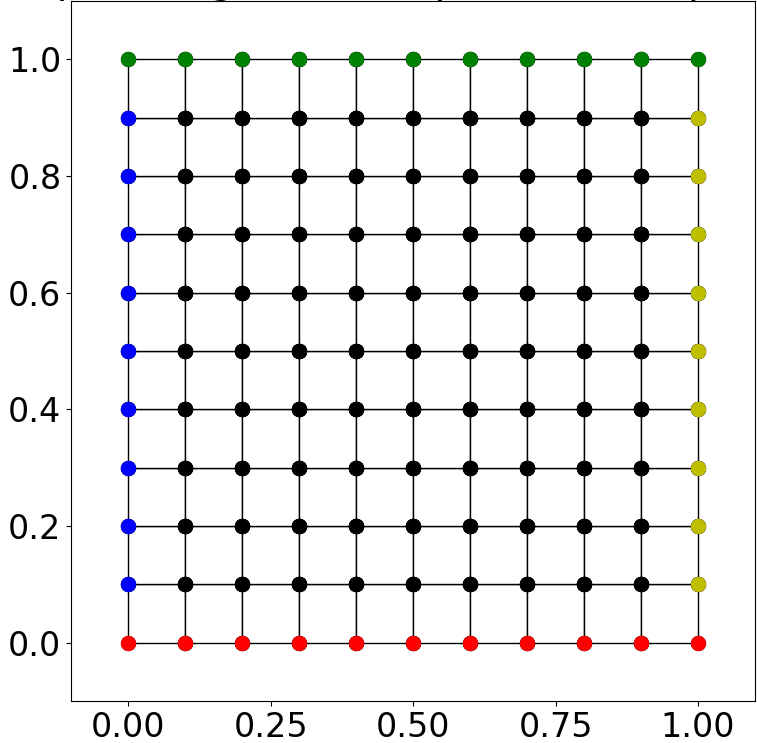
\includegraphics[width=\textwidth]{images/fiber_creation/quad_1.png}%
    \caption{Square, scheme 1}%
    \label{fig:tquad_1}%
  \end{subfigure}
  \begin{subfigure}[t]{0.24\textwidth}%
    \centering%
    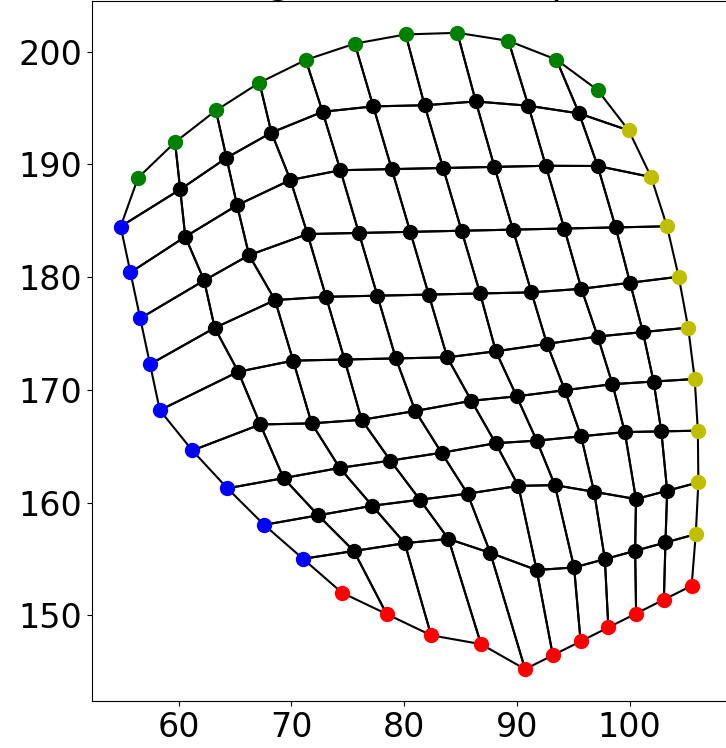
\includegraphics[width=\textwidth, trim=26mm 14mm 6mm 6mm, clip]{images/fiber_creation/mesh_plots/out_0_1_0_w.png}%
    %\caption{}%
    \label{fig:tri_01}%
  \end{subfigure}
  \begin{subfigure}[t]{0.24\textwidth}%
    \centering%
    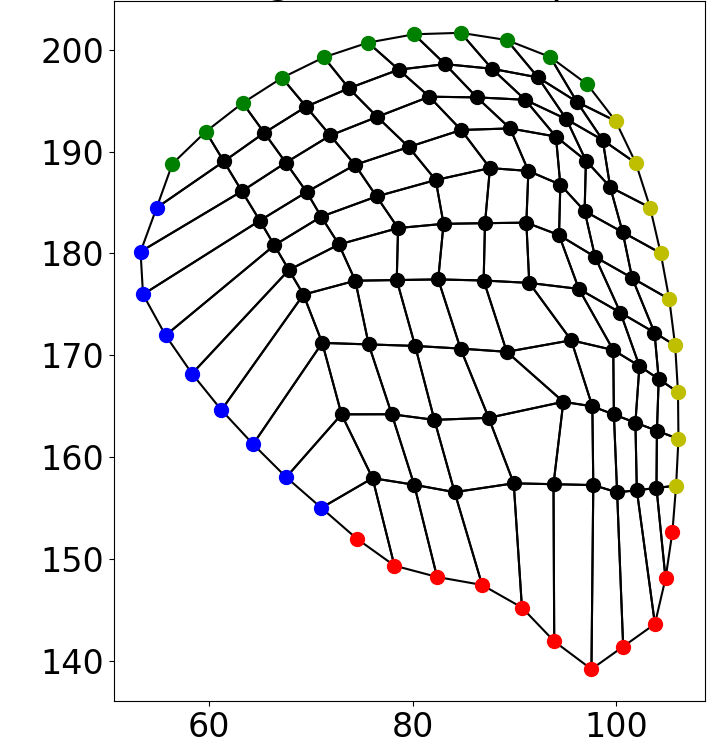
\includegraphics[width=\textwidth, trim=30mm 14mm 6mm 6mm, clip]{images/fiber_creation/mesh_plots/out_1_1_0_w.png}%
    %\caption{}%
    \label{fig:tri_11}%
  \end{subfigure}
  \begin{subfigure}[t]{0.24\textwidth}%
    \centering%
    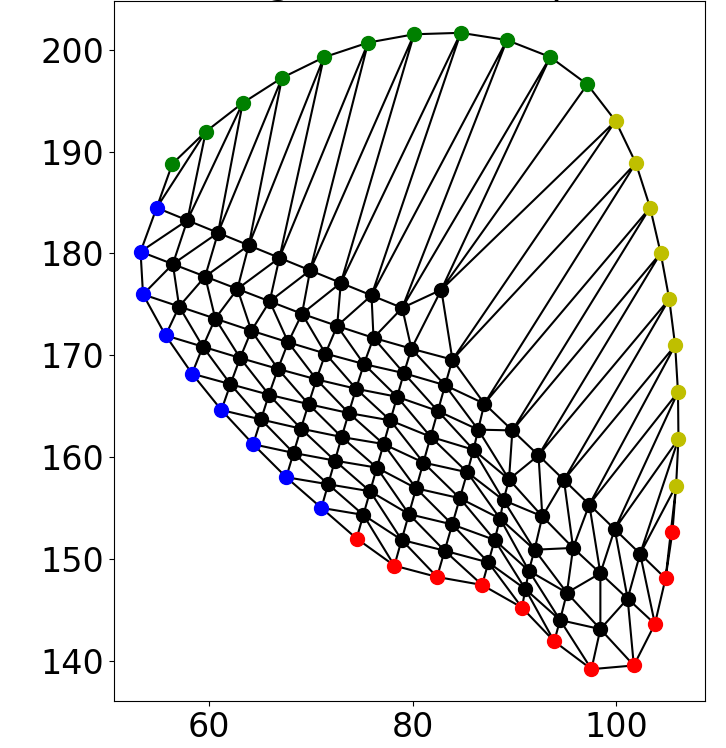
\includegraphics[width=\textwidth, trim=30mm 14mm 6mm 6mm, clip]{images/fiber_creation/mesh_plots/out_2_1_0_w.png}%
    %\caption{}%
    \label{fig:tri_21}%
  \end{subfigure}\\[-4mm]
  
  % square adjusted
  \begin{subfigure}[t]{0.24\textwidth}%
    \centering%
    \includegraphics[width=\textwidth]{images/fiber_creation/quad_2.png}%
    \caption{Square, scheme 2}%
    \label{fig:tquad_2}%
  \end{subfigure}
  \begin{subfigure}[t]{0.24\textwidth}%
    \centering%
    \includegraphics[width=\textwidth, trim=26mm 14mm 6mm 6mm, clip]{images/fiber_creation/mesh_plots/out_0_2_0_w.png}%
    %\caption{}%
    \label{fig:tri_02}%
  \end{subfigure}
  \begin{subfigure}[t]{0.24\textwidth}%
    \centering%
    \includegraphics[width=\textwidth, trim=30mm 14mm 6mm 6mm, clip]{images/fiber_creation/mesh_plots/out_1_2_0_w.png}%
    %\caption{}%
    \label{fig:tri_12}%
  \end{subfigure}
  \begin{subfigure}[t]{0.24\textwidth}%
    \centering%
    \includegraphics[width=\textwidth, trim=30mm 14mm 6mm 6mm, clip]{images/fiber_creation/mesh_plots/out_2_2_0_w.png}%
    %\caption{}%
    \label{fig:tri_22}%
  \end{subfigure}\\[-4mm]
  
  % circle
  \begin{subfigure}[t]{0.24\textwidth}%
    \centering%
    \includegraphics[width=\textwidth]{images/fiber_creation/quad_0.png}%
    \caption{Circle, scheme 1}%
    \label{fig:tquad_0}%
  \end{subfigure}
  \begin{subfigure}[t]{0.24\textwidth}%
    \centering%
    \includegraphics[width=\textwidth, trim=26mm 14mm 6mm 6mm, clip]{images/fiber_creation/mesh_plots/out_0_0_0_w.png}% trim=left bottom right top, clip]
    %\caption{}%
    \label{fig:tri_00}%
  \end{subfigure}
  \begin{subfigure}[t]{0.24\textwidth}%
    \centering%
    \includegraphics[width=\textwidth, trim=26mm 14mm 6mm 6mm, clip]{images/fiber_creation/mesh_plots/out_1_0_0_w.png}%
    %\caption{}%
    \label{fig:tri_10}%
  \end{subfigure}
  \begin{subfigure}[t]{0.24\textwidth}%
    \centering%
    \includegraphics[width=\textwidth, trim=30mm 14mm 6mm 6mm, clip]{images/fiber_creation/mesh_plots/out_2_0_0_w.png}%
    %\caption{}%
    \label{fig:tri_20}%
  \end{subfigure}\\[-4mm]
  
  % circle adjusted
  \begin{subfigure}[t]{0.24\textwidth}%
    \centering%
    \includegraphics[width=\textwidth]{images/fiber_creation/quad_3.png}%
    \caption{Circle, scheme 2}%
    \label{fig:lquad_3}%
  \end{subfigure}
  \begin{subfigure}[t]{0.24\textwidth}%
    \centering%
    \includegraphics[width=\textwidth, trim=30mm 14mm 6mm 6mm, clip]{images/fiber_creation/mesh_plots/out_0_3_0_w.png}%
    %\caption{}%
    \label{fig:tri_03}%
  \end{subfigure}
  \begin{subfigure}[t]{0.24\textwidth}%
    \centering%
    \includegraphics[width=\textwidth, trim=30mm 14mm 6mm 6mm, clip]{images/fiber_creation/mesh_plots/out_1_3_0_w.png}%
    %\caption{}%
    \label{fig:tri_13}%
  \end{subfigure}
  \begin{subfigure}[t]{0.24\textwidth}%
    \centering%
    \includegraphics[width=\textwidth, trim=30mm 14mm 6mm 6mm, clip]{images/fiber_creation/mesh_plots/out_2_3_0_w.png}%
    %\caption{}%
    \label{fig:tri_23}%
  \end{subfigure}
  \caption{Initial triangulations, harmonic maps and final quadrangulations of muscle slices for 3D mesh generation: Meshes in the muscle slice $S_M$ for quadrangulations (rows) and triangulations (columns).}%
  \label{fig:tri_meshes}%
\end{figure}%

% quantitative quality plots of results

%The mesh quality could easily be improved by a smoothing step, e.g., by applying Laplacian smoothing \cite{field1988laplacianSmoothingAndDelaunayTriangulations}. This technique iteratively improves the local mesh quality. Because of the local scheme, the quality of the final result depends on the quality of the initial mesh. 
%Therefore, the following study forgoes additional smoothing steps and evaluates the direct outcome of the meshing algorithm.

Next, a quantitative comparison of the resulting mesh quality for different parameters of the presented algorithm is carried out. 
The algorithm was executed for all variants with 43 slices of the biceps muscle, resulting in 43 meshes for every combination of triangulation method and quadrangulation scheme. To asses the quality of the generated meshes, the edge lengths of the elements were collected and normalized to have a mean of 1 in each mesh. 
The normalization was done to allow for a comparison between meshes with different bounding box sizes.
The standard deviation of the normalized lengths was determined in each mesh. The total mean of all standard deviations was computed. This value is a measure for the quality of the mesh. A low value means that, in every slice, the generated mesh has similar edge lengths and, in consequence, the overall mesh has good quality.

\begin{figure}%
  \centering%
  \includegraphics[width=\textwidth]{images/fiber_creation/mesh_quality.pdf}%
  \caption{3D mesh generation quality assessment: Mesh quality (red, lower is better) and generation runtime (yellow) for the three different triangulation methods and the different parameter space quadrangulation schemes. $\square 1$ and $\square 2$ designate the two quadrangulation schemes on the unit square parameter domain, $\ocircle 1$ and $\ocircle 2$ are the schemes on the unit circle parameter domain, as introduced in \cref{fig:quads}. A low value for the standard deviation of relative element lengths indicates good quality.}%
  \label{fig:mesh_quality}%
\end{figure}

\Cref{fig:mesh_quality} visualizes the results. Three groups of bars are displayed for the three triangulation methods. For every type of mesh in the parameter space, i.e., unit square ($\square$) or unit circle ($\ocircle$) and scheme 1 or 2, the standard deviation is given by the red bar and the generation runtime of the overall algorithm is given by the yellow bar. The corresponding axis labels for standard deviation and duration are given on the left and right of the diagram.

The diagram shows the lowest standard deviation of edges and therefore the best mesh quality for the first triangulation method and the square ($\square 1$ and $\square 2$), with scheme 1 having a slightly better value than scheme 2. This shows that the modified placement of the nodes in scheme 2 has no positive effect compared to scheme 1.
However, from the observations in \cref{fig:tri_triangulations}, it is known that the boundaries are not represented correctly.
This behavior does not influence the result because of the chosen metric of uniform relative edge lengths.
Similarly good results can be seen for scheme 2 in the circular parameter domain and the second and third triangulations.

Moreover, it can be seen that certain connections between parameter domain and suited triangulation scheme exist. The square parameter domain works best with the first triangulation method. The second scheme for the parameter mesh on the unit circle works best with the triangulation methods 2 and 3.

The first scheme for the parameter mesh on the unit circle ($\ocircle 1$) shows bad results for all triangulation methods. This can be explained by looking at the generated meshes in row (\subref{fig:tquad_0}) of \cref{fig:tri_meshes}. By construction, the elements have a bad aspect ratio. This results in the high standard deviation values. However, the generated meshes still look uniform to a certain extent and can be useful in applications where such type of mesh is needed. The score could be improved by adding more nodes in circumferential direction.

The runtime of the algorithm is approximately the same for the different parameter domain meshes. It mainly depends on the triangulation of the slices. The first triangulation using the \emph{SciPy} package takes the most time, followed by the Delaunay refinement. The fastest triangulation is the custom one where only one additional point needs to be placed. In conclusion, when runtime is an issue, the third triangulation should be chosen. It achieves good quality meshes only with the second scheme of the circular parameter domain. This combination also does not suffer from the bad approximation quality of the boundary, as is the case for the unit circle with the first triangulation method.

\Cref{fig:tendon_meshes} shows three structured meshes $\Omega_{T,i}$ for the tendons of the biceps brachii muscle that were created using \cref{alg:serial_algorithm_1}. The tendon at the bottom of the muscle is represented by a single mesh. At the top, there are two tendons that extend the two muscle heads of the biceps. Because the meshes need to be structured, two tendon meshes are created at the top. It can be seen that the algorithm creates meshes with similar sized elements despite the difficult, wound geometry of the surfaces.

\begin{figure}
  \centering
  \begin{tabular}{cc}
    \begin{tabular}[b]{c}
      \begin{subfigure}[b]{0.60\textwidth}%
        \centering%
        \includegraphics[width=\textwidth]{images/fiber_creation/tendon2_.png}
        \caption{Two meshes for the top tendons with $9 \times 9 \times 21 = \num{1701}$ nodes each.}%
        \label{fig:tendon2}%
      \end{subfigure} \\
      \begin{subfigure}[b]{0.60\textwidth}%
        \centering%
        \includegraphics[width=\textwidth]{images/fiber_creation/tendon1.png}
        \caption{One mesh for the bottom tendon with $5 \times 5 \times 25 = \num{525}$ nodes.}%
        \label{fig:tendon1}%
      \end{subfigure}
    \end{tabular}
    &
    \begin{subfigure}[b]{0.30\textwidth}%
      \centering%
      \includegraphics[width=\textwidth]{images/fiber_creation/muscle_with_tendons.png}
      \caption{The tendon meshes in the volume of the whole biceps muscle.}%
      \label{fig:muscle_with_tendons}%
    \end{subfigure}
  \end{tabular}
  \caption{3D mesh generation results: Tendon meshes that were created using the serial algorithm for mesh creation.}%
  \label{fig:tendon_meshes}%
\end{figure}%

\begin{reproduce_no_break}
  The described algorithms are part of the \code{fiber_tracing} examples. Execute the following commands to get the results in this chapter:
  \begin{lstlisting}[columns=fullflexible,breaklines=true,postbreak=\mbox{\textcolor{gray}{$\hookrightarrow$}\space}]
    cd $\$$OPENDIHU_HOME/examples/fiber_tracing/streamline_tracer/scripts
    . run_evaluation.sh
  \end{lstlisting}
  Then, the visualizations will be created under \code{../processed_meshes}. Create \cref{fig:mesh_quality} with \code{plot_mesh_quality.py}.
  How to create the tendon meshes is explained at the end of \cref{sec:repro_tendon_meshes}.
\end{reproduce_no_break}

